\documentclass[11pt]{article}
\usepackage[T1]{fontenc}
\usepackage[utf8]{inputenc}
\usepackage{amsmath,amssymb,amsthm,mathtools,xparse,enumitem,hyperref,tikz,pgfplots}
\pgfplotsset{compat=1.18}
\usepackage[a4paper,margin=25mm]{geometry}
\setlength{\emergencystretch}{3em}
\numberwithin{equation}{section}
\newtheorem{theorem}{Theorem}[section]
\newtheorem{lemma}[theorem]{Lemma}
\newtheorem{proposition}[theorem]{Proposition}
\newtheorem{corollary}[theorem]{Corollary}
\newtheorem{claim}[theorem]{Claim}
\theoremstyle{definition}
\newtheorem{definition}[theorem]{Definition}
\newtheorem{example}[theorem]{Example}
\newtheorem{examples}[theorem]{Examples}
\newtheorem{notation}[theorem]{Notation}
\theoremstyle{remark}
\newtheorem{remark}[theorem]{Remark}
\renewcommand{\theoremautorefname}{Result}
\newcommand{\pqty}[1]{\left(#1\right)}
\newcommand{\bqty}[1]{\left[#1\right]}
\newcommand{\Bqty}[1]{\left\{#1\right\}}
\newcommand{\abs}[1]{\left|#1\right|}
\newcommand{\floor}[1]{\left\lfloor#1\right\rfloor}
\newcommand{\flatfrac}[2]{\frac{#1}{#2}}
\newcommand{\set}[2]{\left\{#1\mid #2\right\}}
\newcommand{\ccintv}[2]{[#1,#2]}
\newcommand{\oointv}[2]{(#1,#2)}
\newcommand{\cointv}[2]{[#1,#2)}
\newcommand{\ocintv}[2]{(#1,#2]}
\newcommand{\functiondomain}[3]{#1:#2\to #3}
\newcommand{\function}[5]{#1:#2\to #3,\quad #4\mapsto #5}
\newcommand{\RR}{\mathbb R}
\newcommand{\NN}{\mathbb N}
\newcommand{\QQ}{\mathbb Q}
\newcommand{\plusinfty}{+\infty}
\newcommand{\minusinfty}{-\infty}
\newcommand{\littleO}{o}
\newcommand{\inverse}{^{-1}}
\newcommand{\transpose}{^{\mathsf T}}
\newcommand{\rightbar}[1]{\left.#1\right|}
\newcommand{\qand}{\quad\text{and}\quad}
\newcommand{\indicator}{\mathbf 1}
\newcommand{\compl}{^{\mathrm c}}
\newcommand{\powerset}{\mathcal P}
\newcommand{\eventSpace}{\mathcal F}
\newcommand{\Prob}{\mathbb P}
\newcommand{\Expt}{\mathbb E}
\DeclareMathOperator{\Var}{Var}
\DeclareMathOperator{\Cov}{Cov}
\DeclareMathOperator{\Corr}{Corr}
\DeclareMathOperator{\img}{im}
\DeclareMathOperator{\diag}{diag}
\newcommand{\indp}{\mathrel{\perp\!\!\!\perp}}
\newcommand{\Conditional}[2]{#1\mid #2}
\newcommand{\bound}[1]{{#1}}
\newcommand{\identityM}{I}
\newcommand{\zeroM}{0}
\newcommand{\posDef}{\succ}
\newcommand{\posDefEq}{\succeq}
\newcommand{\negDef}{\prec}
\newcommand{\negDefEq}{\preceq}
\newcommand{\sNormPdf}{\varphi}
\newcommand{\sNormCdf}{\Phi}
\newcommand{\toProb}{\xrightarrow{\mathbb P}}
\newcommand{\toDist}{\xrightarrow{\mathrm d}}
\newcommand{\toAlmostSure}{\xrightarrow{\mathrm{a.s.}}}
\newcommand{\Bernoulli}{\operatorname{Bernoulli}}
\newcommand{\Binomial}{\operatorname{Bin}}
\newcommand{\Multinomial}{\operatorname{Multinomial}}
\newcommand{\Poisson}{\operatorname{Poisson}}
\newcommand{\GeomOne}{\operatorname{Geom}_1}
\newcommand{\GeomZero}{\operatorname{Geom}_0}
\newcommand{\Exponential}{\operatorname{Exp}}
\newcommand{\Uniform}{\operatorname{Unif}}
\newcommand{\Normal}{\mathcal N}
\NewDocumentCommand{\vb}{s m}{\boldsymbol{#2}}
\newcommand{\pmqty}[1]{\begin{pmatrix}#1\end{pmatrix}}
\NewDocumentCommand{\dd}{o m}{\,\mathrm d\IfNoValueF{#1}{^{#1}}#2}
\NewDocumentCommand{\dv}{s o m g}{\IfNoValueTF{#4}{\frac{\mathrm d\IfNoValueF{#2}{^{#2}}}{\mathrm d#3\IfNoValueF{#2}{^{#2}}}}{\IfNoValueTF{#2}{\frac{\mathrm d#3}{\mathrm d#4}}{\frac{\mathrm d^{#2}#3}{\mathrm d#4^{#2}}}}}
\NewDocumentCommand{\pdv}{o m m}{\IfNoValueTF{#1}{\frac{\partial #2}{\partial #3}}{\frac{\partial^{#1}#2}{\partial #3^{#1}}}}
\title{Probability: Distributions, Conditioning, Random Processes and Limit Theorems}
\author{Notes by Eason Shao; lectures by P. Sousi}
\date{Cambridge Part IA, Lent Term 2026; revised 2026-09-28}
\begin{document}
\maketitle
\paragraph{Provenance and scope.}
Revised unofficial notes from \texttt{ia-dpmms-probability-lt-2026}, by Eason
Shao, based on lectures by P. Sousi; not endorsed by the lecturer.
The fifteen mathematical chapters are retained, with corrected formulas,
explicit hypotheses and locally defined macros replacing the unavailable
personal package. The distribution tables are recast as structured entries.
This is a targeted revision, not an exhaustive mathematical certification.
Source: \url{https://github.com/EasonSYC/ia-dpmms-probability-lt-2026}.
\paragraph{Conventions and retrieval context.}
\(\NN=\{1,2,\ldots\}\), \(\NN_0=\{0,1,2,\ldots\}\).
\(\GeomOne(p)\) counts trials including the first success; \(\GeomZero(p)\)
counts failures before it, always with \(0<p\le1\).
The parameter \(\lambda\) of exponential and gamma laws is a rate.
\(\mathcal N(\mu,\sigma^2)\) uses variance as second parameter.
Expectations are Lebesgue integrals; signed finite expectation means absolute
integrability. Probabilities refer to measurable events, and functions of
non-discrete variables are Borel measurable. Densities are identified up to
Lebesgue-null sets. Conditional expectations are identified almost surely.
In PMFs, PGFs and products, use \(0^0=1\).
For retrieval retain the domain, hypotheses, support and parameterisation with
each statement, together with its proof and referenced definitions. A compilation
check does not validate every mathematical argument.
\tableofcontents
\section{Axiomatic Approach}\label{probability-section-01}

\begin{definition}[\(\sigma\)-Algebra]\label{probability-definition-001}
    \label{probability-def:sigma-algebra}%
    Suppose \(\Omega\) is a set, and \(\eventSpace \subseteq \powerset\pqty{\Omega}\) is a collection of subsets of \(\Omega\). We say \(\eventSpace\) is a \emph{\(\sigma\)-algebra}, if the following hold:
    \begin{enumerate}
        \item \(\Omega \in \eventSpace\);
        \item if \(A \in \eventSpace\), then the complement \(A\compl \in \eventSpace\);
        \item if \(\pqty{A_n}_{n \in \NN}\) is a countable collection of sets in \(\eventSpace\) (i.e. \(A_n \in \eventSpace\) for all \(n \in \NN\)), then
        \[
            \bigcup_{n \in \NN} A_n \in \eventSpace.
        \]
    \end{enumerate}
\end{definition}

\begin{definition}[Probability Measure]\label{probability-definition-002}
    \label{probability-def:probability-measure}%
    Suppose \(\eventSpace\) is a \(\sigma\)-algebra on \(\Omega\). A function
    \[
        \functiondomain{\Prob}{\eventSpace}{\ccintv{0}{1}}
    \]
    is called a \emph{probability measure} if
    \begin{enumerate}
        \item \(\Prob\pqty{\Omega} = 1\);
        \item for any countable disjoint collection \(\pqty{A_n}_{n \in \NN}\) in \(\eventSpace\), we have
        \[
            \Prob\pqty{\bigcup_{n \in \NN} A_n} = \sum_{n \in \NN} \Prob\pqty{A_n}.
        \]
    \end{enumerate}

    The value of \(\Prob\pqty{A}\) for some \(A \in \eventSpace\) is the \emph{probability of \(A\)}.
\end{definition}

\begin{definition}[Probability Space]\label{probability-definition-003}
    \label{probability-def:probability-space}%
    For a set \(\Omega\), a \(\sigma\)-algebra \(\eventSpace\) on \(\Omega\), and a probability measure \(\Prob\) on \(\eventSpace\) and \(\Omega\), the triple
    \[
        \pqty{\Omega, \eventSpace, \Prob}
    \]
    is a \emph{probability space}.
\end{definition}

\begin{definition}[Outcomes, Events]\label{probability-definition-004}
    \label{probability-def:outcome-event}%
    The elements of the set \(\Omega\) are called \emph{outcomes}, and the elements of the \(\sigma\)-algebra \(\eventSpace\) are called \emph{events}.
\end{definition}

\begin{remark}\label{probability-remark-001}
    In the elementary countable models in these notes we choose \(\eventSpace\) to be \(\powerset\pqty{\Omega}\), the set of all subsets of \(\Omega\). This is a modelling choice, not a requirement imposed by the definition of a probability space.
\end{remark}

We note that we talk about probability of \emph{events}, rather than \emph{outcomes} -- the probability function is defined from \(\eventSpace\), the \(\sigma\)-algebra.

We may conclude some properties of the probability measure \(\Prob\) from the definition.

\begin{proposition}[Properties of \(\Prob\)]\label{probability-proposition-001}
    \label{probability-prop:properties-prob}%
    \begin{itemize}
        \item \(\Prob\pqty{A\compl} = 1 - \Prob\pqty{A}\).
        \item \(\Prob\pqty{\emptyset} = 0\).
        \item \(\Prob\pqty{A} \leq \Prob\pqty{B}\) if \(A \subseteq B\).
        \item \(\Prob\pqty{A \cup B} = \Prob\pqty{A} + \Prob\pqty{B} - \Prob\pqty{A \cap B}\).
    \end{itemize}
\end{proposition}

\section{Combinatorics}\label{probability-section-02}

\subsection{Equally Likely Outcomes}
Now we consider some examples of probability spaces, where the outcomes are finite, and all outcomes are equally likely.

\begin{example}[Rolling a Fair Die]\label{probability-example-001}
    \label{probability-ex:rolling-a-fair-die}%
    We consider the outcomes \(\Omega = \Bqty{1, 2, \ldots, 6}\), and \(\eventSpace = \powerset\pqty{\Omega}\) for all subsets of \(\Omega\) (since \(\Omega\) is countable).
        
    We naturally take for all \(\omega \in \Omega\),
    \[
        \Prob\pqty{\Bqty{\omega}} = \frac{1}{6},
    \]
    and for all \(A \subseteq \Omega\), we take
    \[
        \Prob\pqty{A} = \frac{\abs{A}}{6}.
    \]

    All outcomes are equally likely.
\end{example}

Lots of situations are like this in real life, and we refer to such setup as \emph{classical probability}, with \emph{equally likely outcomes}.

\begin{definition}[Equally Likely Outcomes]\label{probability-definition-005}
    \label{probability-def:equally-likely-outcomes}
Assume \(n\ge1\), so the finite sample space is nonempty.
%
    For any finite set \(\Omega = \Bqty{\omega_1, \omega_2, \ldots, \omega_n}\), take \(\eventSpace = \powerset\pqty{\Omega}\). We define the probability measure to be
    \[
        \function{\Prob}{\eventSpace}{\ccintv{0}{1}}{A}{\frac{\abs{A}}{\abs{\Omega}}.}
    \]

    This is called the \emph{uniform probability distribution}.
\end{definition}

This models the experiment of picking a \emph{random} element of \(\Omega\). For all \(\omega \in \Omega\),
\[
    \Prob\pqty{\Bqty{\omega}} = \frac{1}{\abs{\Omega}}
\]

We look at some more examples on calculating the probability under such setup. Effectively, those are combinatorial problems counting the size of sets.

This example is more about counting the size of the \emph{sample space} which is the denominator.

\begin{example}[Picking Balls from a Bag]\label{probability-example-002}
    \label{probability-ex:picking-balls-from-bag}%
    Suppose we have \(n\) balls labelled \(\Bqty{1, \ldots, n}\), and they are indistinguishable by touch. Pick \(k \leq n\) balls \emph{at random} (any outcome is equally likely) without replacement. We let the outcomes be
    \[
        \Omega = \set{A \subseteq \Bqty{1, 2, \ldots, n}}{\abs{A} = k}
    \]
    and hence
    \[
        \abs{\Omega} = \binom{n}{k}.
    \]

    Hence, for any \(\omega \in \Omega\), we have
    \[
        \Prob\pqty{\Bqty{\omega}} = \frac{1}{\binom{n}{k}}.
    \]
\end{example}

The following examples also require counting on the numerator, which is the cardinality of the event.

\begin{example}[Deck of Cards]\label{probability-example-003}
    \label{probability-ex:deck-of-cards}%
    In a well-shuffled deck of 52 cards, take
    \[
        \Omega = \Bqty{\text{all permutations of 52 cards}}
    \]
    and hence
    \[
        \abs{\Omega} = 52! \approx 8.0658\times10^{67}.
    \]
    
    Take \(\eventSpace = \powerset\pqty{\Omega}\). Then
    \[
        \Prob\pqty{\text{top 2 cards are aces}} = \frac{4 \times 3 \times 50!}{52!}.
    \]
\end{example}

The next example uses results on set cardinalities.

\begin{example}[Largest Digit]\label{probability-example-004}
    \label{probability-ex:largest-digit}
Assume \(n\ge1\), independent uniform digits, and \(k\in\{0,\ldots,9\}\). Set \(A_{-1}=\emptyset\).
%
    Consider a string of \(n\) random digits from \(0, 1, \ldots, 9\). Let
    \[
        \Omega = \Bqty{0, 1, \ldots, 9}^n,
    \]
    and we have \(\abs{\Omega} = 10^n\).

    Let the event \(A_k = \Bqty{\text{no digit exceeds }k}\), then
    \[
        \Prob\pqty{A_k} = \frac{\pqty{k + 1}^{n}}{10^n}.
    \]

    Now we consider the event \(B_k = \Bqty{\text{the largest digit is equal to }k}\), then note \(B_k = A_k \setminus A_{k - 1}\), so
    \[
        \Prob\pqty{B_k} = \Prob\pqty{A_k \setminus A_{k - 1}} = \Prob\pqty{A_k} - \Prob\pqty{A_{k - 1}} = \frac{\pqty{k + 1}^n - k^n}{10^n}.
    \]
\end{example}

\begin{example}[Birthday Problem]\label{probability-example-005}
    \label{probability-ex:birthbay-problem}%
The product formula below is for \(1\le n\le365\). For \(n>365\), the collision probability is \(1\).
    There are \(n\) people. What is the probability that at least 2 of them share the same birthday?
        
    Assume birthdays are independent and each birthday is equally likely to be one of \(\Bqty{1, 2, \ldots, 365}\). Take
    \[
        \Omega = \Bqty{1, 2, \ldots, 365}^n,
    \]
    and take \(\eventSpace = \powerset\pqty{\Omega}\). Hence, for all \(\omega \in \Omega\), we have
    \[
        \Prob\pqty{\Bqty{\omega}} = \frac{1}{365^n}.
    \]

    Consider the event \(A = \Bqty{\text{at least 2 people have the same birthday}}\).

    Then \(A\compl = \Bqty{\text{all }n\text{ birthdays are different}}\). Hence,
    \[
        \Prob\pqty{A\compl} = \frac{365 \times 364 \times \cdots \times \pqty{365 - n + 1}}{365^n}
    \]
    and hence
    \[
        \Prob\pqty{A} = 1 - \Prob\pqty{A\compl}.
    \]

    Note that \(n = 22\) gives \(\Prob\pqty{A} \approx 0.476\), and \(n = 23\) gives \(\Prob\pqty{A} \approx 0.507\).
\end{example}

\subsection{Combinatorial Analysis}
We start off by investigating some easy problems in combinatorics.

\begin{example}[Partitioning Sets into Fixed Sizes]\label{probability-example-006}
    \label{probability-ex:partition-sets-given-size}%
    We first consider \(\Omega\) being a finite set with \(\abs{\Omega} = n\). We want to partition \(\Omega\) into \(k\) labelled disjoint subsets \(\Omega_1, \Omega_2, \ldots, \Omega_k\) with \(\abs{\Omega_i} = n_i\) for \(\sum_{i = 1}^{k} n_i = n\).

    Let \(M\) be the number of ways to do this. We have
    \begin{align*}
        M &= \binom{n}{n_1} \times \binom{n - n_1}{n_2} \times \cdots \times \binom{n - \pqty{n_1 + \cdots + n_{k - 1}}}{n_k} \\
        &= \frac{n!}{n_1! n_2! \cdots n_k!}.
    \end{align*}
\end{example}

\begin{definition}[Multinomial Coefficient]\label{probability-definition-006}
    \label{probability-def:multinomial-coeff}
Here \(n_i\in\NN_0\), \(\sum_i n_i=n\), and the categories are labelled.
%
    The \emph{multinomial coefficient} is defined as
    \[
        \binom{n}{n_1, n_2, \ldots, n_k} = \frac{n!}{n_1! n_2! \cdots n_k!}.
    \]
\end{definition}

\begin{examples}[Increasing and Strictly Increasing Functions]\label{probability-examples-001}
    \label{probability-ex:increasing-functions}%
    We say \(f\) is \emph{strictly increasing} if \(x < y\) implies \(f\pqty{x} < f\pqty{y}\), and \(f\) is \emph{(weakly) increasing}, if \(x \leq y\) implies \(f\pqty{x} \leq f\pqty{y}\).

    Let \(\functiondomain{f}{\Bqty{1, 2, \ldots, k}}{\Bqty{1, 2, \ldots, n}}\).
    
    \begin{enumerate}
        \item \textit{Strictly Increasing Functions.} Let \(k \leq n\). How many strictly increasing functions \(f\) are there? Such a function is uniquely determined by its range, so there are \(\binom{n}{k}\) of them.
        \item \textit{Increasing Functions.} How many increasing functions \(f\) are there?
        
        Let the function space
        \[
            \eventSpace\pqty{k, n} = \set{f}{\functiondomain{f}{\Bqty{1, 2, \ldots, k}}{\Bqty{1, 2, \ldots, n}}}.
        \]
        
        We define a bijection
        \[
            \set{f \in \eventSpace\pqty{k, n}}{f \text{ is increasing}} \to \set{g \in \eventSpace\pqty{k, n + k - 1}}{g \text{ is strictly increasing}},
        \]
        where \(g\pqty{i} = f\pqty{i} + i - 1\) that is strictly increasing. Hence, there are
        \[
            \binom{n + k - 1}{k}
        \]
        such increasing functions in \(\eventSpace\pqty{k, n}\).
    \end{enumerate}
\end{examples}

\subsection{Stirling's Formula}

The following asymptotic formula is very useful in the study of probability. A proof is included below.

\begin{definition}[Asymptotic]\label{probability-definition-007}
    \label{probability-def:asymptotic}
Assume \(b_n\ne0\) for all sufficiently large \(n\).
%
    For two sequences \(\pqty{a_n}, \pqty{b_n}\), we say \(\pqty{a_n}\) is \emph{asymptotic} to \(\pqty{b_n}\), denoted as
    \[
        a_n \sim b_n
    \]
    as \(n \to \infty\), if \(\frac{a_n}{b_n} \to 1\) as \(n \to \infty\).
\end{definition}

\begin{theorem}[Stirling's Formula]\label{probability-theorem-001}
    \label{probability-thm:stirling-formula}%
    We have
    \[
        n! \sim n^n \sqrt{2 \pi n} \cdot e^{-n},
    \]
    as \(n \to \infty\).
\end{theorem}

The following useful consequence also has a direct proof.

\begin{corollary}\label{probability-corollary-001}
    \label{probability-cor:weaker-statement-of-stirling}%
    We have \(\log \pqty{n!} \sim n \log n\) as \(n \to \infty\).
\end{corollary}

\begin{proof}\label{probability-proof-001}
    Define
    \[
        l_n = \log\pqty{n!} = \log 2 + \cdots + \log n.
    \]

    For all \(x \geq 1\), denote \(\floor{x}\) as the integer part of \(x\). We have
    \[
        \log \floor{x} \leq \log x \leq \log \floor{x + 1}.
    \]

    We integrate this inequality from \(1\) to \(n\), and hence, we have
    \[
        \sum_{k = 1}^{n - 1} \log k \leq \int_{1}^{n} \log x \dd{x} \leq \sum_{k = 1}^{n} \log k
    \]
    and hence we have
    \[
        l_{n - 1} \leq n \log n - n + 1 \leq l_n.
    \]

    Therefore, rearranging this gives
    \[
        n \log n - n + 1 \leq l_n \leq \pqty{n + 1} \log \pqty{n + 1} - \pqty{n + 1} + 1,
    \]
    and dividing this through by \(n \log n\) gives
    \[
        \frac{l_n}{n \log n} \to 1
    \]
    as \(n \to \infty\).
\end{proof}

We first show that Stirling's Formula is true, up to some constant (which would turn out to be \(\sqrt{2\pi}\)). A lemma that could be useful is a result that comes from integration by parts.

\begin{lemma}\label{probability-lemma-001}
    \label{probability-lem:some-integration-formula}%
    For \(a<b\) and \(f\in C^2([a,b])\), we have
    \[
        \int_a^b f\pqty{x} \dd{x} = \frac{f\pqty{a} + f\pqty{b}}{2} \cdot \pqty{b - a} - \frac{1}{2} \int_a^b \pqty{x - a} \pqty{b - x} f''\pqty{x} \dd{x}.
    \]
\end{lemma}

\begin{proof}\label{probability-proof-002}
    Using integration by parts twice.
\end{proof}


\begin{lemma}[Stirling's Formula with Constant]\label{probability-lemma-002}
    \label{probability-lem:stirling-formula-constant}%
    We have
    \[
        n! \sim A n^n \sqrt{n} \cdot e^{-n},
    \]
    as \(n \to \infty\), for some real number \(A > 0\).
\end{lemma}

\begin{proof}\label{probability-proof-003}
    Take \(f\pqty{x} = \log x\), with \(a = k\), \(b = k + 1\), for \(k \in \NN\). Using \autoref{probability-lem:some-integration-formula}, we have
    \[
        \int_{k}^{k + 1} \log x \dd{x} = \frac{\log k + \log\pqty{k + 1}}{2} + \frac{1}{2} \int_{k}^{k + 1} \frac{\pqty{x - k} \pqty{k + 1 - x}}{x^2} \dd{x}.
    \]

    Summing this from \(k = 1\) to \(n - 1\) gives
    \[
        \int_{1}^{n} \log x \dd{x} = \frac{\log \pqty{n - 1}! + \log \pqty{n!}}{2} + \sum_{k = 1}^{n - 1} a_k,
    \]
    where
    \[
        a_k = \frac{1}{2} \int_{0}^{1} \frac{x \pqty{1 - x}}{\pqty{x + k}^2} \dd{x}.
    \]

    Hence, we have
    \[
        n \log n - n + 1 = \log\pqty{n!} - \frac{\log n}{2} + \sum_{k = 1}^{n - 1} a_k
    \]

    Therefore,
    \[
        \log \pqty{n!} = n \log n - n + 1 + \frac{\log n}{2} - \sum_{k = 1}^{n - 1} a_k,
    \]
    and hence
    \[
        n! = n^n \cdot e^{-n} \cdot \sqrt{n} \cdot \exp\pqty{1 - \sum_{k = 1}^{n - 1} a_k}.
    \]

    Now, we have
    \[
        a_k = \frac{1}{2} \int_{0}^{1} \frac{x \pqty{1 - x}}{\pqty{x + k}^2} \dd{x} \leq \frac{1}{2k^2} \int_{0}^{1} x\pqty{1 - x} \dd{x} = \frac{1}{12k^2}.
    \]

    Therefore,
    \[
        \sum_{k = 1}^{\infty} a_k < \infty.
    \]

    Let \(A = \exp\pqty{1 - \sum_{k = 1}^{\infty} a_k}\). Therefore,
    \[
        n! = n^n \cdot e^{-n} \cdot \sqrt{n} \cdot A \cdot \exp\pqty{\sum_{k = n}^{\infty} a_k}.
    \]

    The \(\exp\pqty{\sum_{k = n}^{\infty} a_k}\) will converge to \(1\) as \(n \to \infty\), since the inner sum converges to \(0\).

    We have showed that
    \[
        \frac{n!}{n^n \cdot e^{-n} \cdot \sqrt{n}} \to A
    \]
    as \(n \to \infty\), as desired.
\end{proof}

To finish the proof of \autoref{probability-thm:stirling-formula} (Stirling's Formula), we want to find \(A\). An asymptotic analysis on the binomial coefficient \(2^{-2n} \binom{2n}{n}\) would be useful, and one method to do this is to use the expansion of the binomial coefficient.

\begin{lemma}[Asymptotic for \(2^{-2n} \binom{2n}{n}\), using Factorials]\label{probability-lemma-003}
    \label{probability-lem:asymptotic-binomial-factorial}%
    We have
    \[
        2^{-2n} \binom{2n}{n} \sim \frac{\sqrt{2}}{A \sqrt{n}}
    \]
    for the \(A\) above, in \autoref{probability-lem:stirling-formula-constant}.
\end{lemma}

\begin{proof}\label{probability-proof-004}
    Notice that
    \begin{align*}
        2^{-2n} \binom{2n}{n} &= 2^{-2n} \cdot \frac{\pqty{2n}!}{n! \cdot n!} \\
        &\sim \frac{2^{-2n} \cdot \pqty{2n}^{2n} \cdot e^{-2n} \cdot \sqrt{2n} \cdot A}{n^n \cdot e^{-n} \cdot \sqrt{n} \cdot A \cdot n^n \cdot e^{-n} \cdot \sqrt{n} \cdot A} \\
        &= \frac{\sqrt{2}}{A \sqrt{n}}.
    \end{align*}
\end{proof}

Another way to study the asymptotic behaviour of this function, is to relate this with the Wallis Integral.

\begin{lemma}[The Wallis Integrals]\label{probability-lemma-004}
    \label{probability-lem:wallis-integral}%
    Let
    \[
        I_n = \int_{0}^{\frac{\pi}{2}} \cos^n \theta \dd{\theta}
    \]
    be the Wallis Integrals. We have
    \[
        I_{2n} = \frac{\pi}{2} \cdot 2^{-2n} \cdot \binom{2n}{n},
    \]
    and
    \[
        I_{2n + 1} = \frac{1}{2n + 1} \cdot \pqty{2^{-2n} \cdot \binom{2n}{n}}\inverse.
    \]
\end{lemma}

\begin{proof}\label{probability-proof-005}
    We notice \(I_0 = \frac{\pi}{2}\) and \(I_1 = 1\). Integration by parts gives us
    \[
        I_n = \frac{n - 1}{n} \cdot I_{n - 2},
    \]
    so
    \begin{align*}
        I_{2n} &= \frac{2n - 1}{2n} \cdot I_{2n - 2} \\
        &= \cdots \\
        &= \frac{\pqty{2n - 1} \cdot \pqty{2n - 3} \cdots 3 \cdot 1}{\pqty{2n} \cdot \pqty{2n - 2} \cdots 2} I_0 \\
        &= \frac{\pqty{2n} \cdot \pqty{2n - 1} \cdot \pqty{2n - 2} \cdot \pqty{2n - 3} \cdots 3 \cdot 2 \cdot 1}{2n \cdot 2n \cdot \pqty{2n - 2} \cdot \pqty{2n - 2} \cdots 2 \cdot 2} \cdot \frac{\pi}{2} \\
        &= \frac{\pqty{2n}!}{2^{2n} \cdot n! \cdot n!} \cdot \frac{\pi}{2} \\
        &= \frac{\pi}{2} \cdot 2^{-2n} \cdot \binom{2n}{n},
    \end{align*}
    so we have
    \[
        I_{2n} = \frac{\pi}{2} \cdot 2^{-2n} \cdot \binom{2n}{n}.
    \]

    Similarly, we have
    \[
        I_{2n + 1} = \frac{2n \cdot \pqty{2n - 2} \cdots 4 \cdot 2}{\pqty{2n + 1} \cdot \pqty{2n - 1} \cdots 3 \cdot 1} I_1 = \frac{1}{2n + 1} \cdot \pqty{2^{-2n} \cdot \binom{2n}{n}}\inverse.
    \]

\end{proof}

\begin{corollary}[Asymptotic for \(2^{-2n} \binom{2n}{n}\), using Wallis]\label{probability-corollary-002}
    \label{probability-cor:asymptotic-binomial-wallis}%
    We have
    \[
        2^{-2n} \binom{2n}{n} \sim \frac{1}{\sqrt{\pi n}}.
    \]
\end{corollary}

\begin{proof}\label{probability-proof-006}
    We use \autoref{probability-lem:wallis-integral}. 

    Notice that we have \(\frac{I_n}{I_{n - 2}} \to 1\) as \(n \to \infty\).

    Note that \(I_n\) is decreasing in \(n\), so
    \[
        \frac{I_{2n}}{I_{2n + 1}} \leq \frac{I_{2n - 1}}{I_{2n + 1}} \to 1
    \]
    and
    \[
        \frac{I_{2n}}{I_{2n + 1}} \geq \frac{I_{2n}}{I_{2n - 1}} \to 1,
    \]
    so we have \(\frac{I_{2n}}{I_{2n + 1}} \to 1\) as \(n \to \infty\).

    Hence,
    \[
        \frac{\frac{\pi}{2} \cdot 2^{-2n} \cdot \binom{2n}{n}}{\frac{1}{2n + 1} \cdot \pqty{2^{-2n} \cdot \binom{2n}{n}}\inverse} \to 1
    \]
    which gives
    \[
        \pqty{2^{-2n} \cdot \binom{2n}{n}}^2 \sim \frac{1}{\pi n}
    \]
    as \(n \to \infty\), as desired.
\end{proof}

Now we are ready to find \(A\), and give a proof of the original statement in \autoref{probability-thm:stirling-formula} (Stirling's formula).

\begin{proof}[\proofname\ of \autoref{probability-thm:stirling-formula} (Stirling's Formula)]\label{probability-proof-007}
    From \autoref{probability-lem:stirling-formula-constant}, it remains to show that \(A = \sqrt{2 \pi}\).
    
    Using the result in \autoref{probability-lem:asymptotic-binomial-factorial}, we have
    \[
        2^{-2n} \binom{2n}{n} \sim \frac{\sqrt{2}}{A \sqrt{n}}.
    \]

    From \autoref{probability-cor:asymptotic-binomial-wallis}, we also have
    \[
        2^{-2n} \binom{2n}{n} \sim \frac{1}{\sqrt{\pi n}}.
    \]
    
    This then implies \(A = \sqrt{2 \pi}\), which shows the result as desired.
\end{proof}



\section{Fundamentals}\label{probability-section-03}

\subsection{Properties of the Probability Measure}

Let \(\pqty{\Omega, \eventSpace, \Prob}\) be a probability space. We give some useful properties of the probability measure \(\Prob\), other than those on the example sheets.

\begin{proposition}[Countable Subadditivity]\label{probability-proposition-002}
    \label{probability-prop:countable-subadditivity}%
    If \(\pqty{A_n}\) is a collection in \(\eventSpace\), then
    \[
        \Prob\pqty{\bigcup_{n \in \NN} A_n} \leq \sum_{n \in \NN} \Prob\pqty{A_n}.
    \]
\end{proposition}

\begin{proof}\label{probability-proof-008}
    Define \(B_1 = A_1\), and for \(n \geq 2\), we let
    \[
        B_n = A_n \setminus \pqty{A_1 \cup A_2 \cup \cdots \cup A_{n - 1}}.
    \]

    Then \(\pqty{B_n}\) is a disjoint collection of sets in \(\eventSpace\), and we have
    \[
        \bigcup_{n \in \NN} B_n = \bigcup_{n \in \NN} A_n,
    \]
    so by the countable additivity property (see \autoref{probability-def:probability-measure}, second point), we have
    \[
        \Prob\pqty{\bigcup A_n} = \Prob\pqty{\bigcup B_n} = \sum \Prob\pqty{B_n} \leq \sum \Prob\pqty{A_n}
    \]
    since \(B_n \subseteq A_n\).
\end{proof}

\begin{proposition}[Continuity of Probability Measure]\label{probability-proposition-003}
    \label{probability-prop:continuity-of-probability-measure}%
    For some \emph{increasing} sequence of events \(\pqty{A_n}_{n \in \NN}\) in \(\eventSpace\) (i.e., we have \(A_n \subseteq A_{n + 1}\) for all \(n \in \NN\)), then we have \(\pqty{\Prob\pqty{A_n}}\) is increasing in \(n\), and converges to the limit
    \[
        \Prob\pqty{A_n} \to \Prob\pqty{\bigcup_{n = 1}^{\infty} A_n}.
    \]
\end{proposition}

\begin{proof}\label{probability-proof-009}
    We define \(B_1 = A_1\), and for \(n \geq 2\), take
    \[
        B_n = A_n \setminus \bigcup_{m = 1}^{n - 1} A_m.
    \]

    Then \(\pqty{B_n}\) are disjoint, and we have
    \[
        \bigcup_{k = 1}^{n} B_k = A_n,
    \]
    so
    \[
        \Prob\pqty{A_n} = \Prob\pqty{\bigcup_{k = 1}^{n} B_k} = \sum_{k = 1}^{n} \Prob\pqty{B_k} \to \sum_{k = 1}^{\infty} \Prob\pqty{B_k}.
    \]

    By the countable additivity property, we have
    \[
        \Prob\pqty{\bigcup_{k = 1}^{\infty} B_k} = \sum_{k = 1}^{\infty} \Prob\pqty{B_k},
    \]
    and we also have
    \[
        \bigcup_{k = 1}^{\infty} B_k = \bigcup_{k = 1}^{\infty} A_k,
    \]
    Therefore
    \[
        \sum_{k = 1}^{\infty} \Prob\pqty{B_k} = \Prob\pqty{\bigcup_{k = 1}^{\infty} A_k},
    \]
    which finishes our proof.
\end{proof}

\begin{corollary}[Continuity of Probability Measure for Decreasing Events]\label{probability-corollary-003}
    \label{probability-cor:continuity-probability-measure-decreasing-sequence}%
     For some \emph{decreasing} sequence of events \(\pqty{A_n}_{n \in \NN}\) in \(\eventSpace\) (i.e., we have \(A_n \supseteq A_{n + 1}\) for all \(n \in \NN\)), then we have \(\pqty{\Prob\pqty{A_n}}\) is decreasing in \(n\), and converges to the limit
    \[
        \Prob\pqty{A_n} \to \Prob\pqty{\bigcap_{n = 1}^{\infty} A_n}.
    \]
\end{corollary}

\begin{proof}\label{probability-proof-010}
    We apply \autoref{probability-prop:continuity-of-probability-measure} by taking the complements.
\end{proof}

\begin{remark}\label{probability-remark-002}
    There is \emph{no} topology involved in play here -- this continuity is different, and the definition we gave above is what is meant for this probability measure.
\end{remark}

We recall that in terms of the cardinality (the cardinality measure on finite sets) that we have the Inclusion--Exclusion Principle. A similar formula holds for two events, \(A, B \in \eventSpace\), which says
\[
    \Prob\pqty{A \cup B} = \Prob\pqty{A} + \Prob\pqty{B} - \Prob\pqty{A \cap B}.
\]

Applying this again to three events \(A, B, C \in \eventSpace\), we have
\begin{align*}
    \Prob\pqty{A \cup B \cup C} &=  \Prob\pqty{\pqty{A \cup B} \cup C}\\
    &= \Prob\pqty{A \cup B} + \Prob\pqty{C} - \Prob\pqty{\pqty{A \cap C} \cup \pqty{B \cap C}} \\
    &= \Prob\pqty{A} + \Prob\pqty{B} + \Prob\pqty{C} - \Prob\pqty{A \cap B} - \Prob\pqty{A \cap C} - \Prob\pqty{B \cap C} + \Prob\pqty{A \cap B \cap C}.
\end{align*}

This leads to \autoref{probability-thm:inclusion-exclusion}, the Inclusion--Exclusion Formula.

\begin{theorem}[Inclusion--Exclusion Formula]\label{probability-theorem-002}
    \label{probability-thm:inclusion-exclusion}%%
    If we have events \(A_1, A_2, \ldots, A_n\in\eventSpace\), then we have
    \[
        \Prob\pqty{\bigcup_{i = 1}^{n} A_i} = \sum_{k = 1}^{n} \pqty{-1}^{k + 1} \sum_{1 \leq i_1 < \cdots < i_k \leq n} \Prob\pqty{A_{i_1} \cap A_{i_2} \cap \cdots \cap A_{i_k}}.
    \]
\end{theorem}

\begin{proof}\label{probability-proof-011}
    This holds for \(n = 2\) events. Assume it holds for \(n - 1\) events.

    We have
    \begin{align*}
        \Prob\pqty{\bigcup_{i = 1}^{n} A_i} &= \Prob\pqty{\bigcup_{i = 1}^{n - 1} A_i \cup A_n} \\
        &= \Prob\pqty{\bigcup_{i = 1}^{n - 1} A_i} + \Prob\pqty{A_n} - \Prob\pqty{\bigcup_{i = 1}^{n - 1} A_i \cap A_n} \\
        &= \Prob\pqty{\bigcup_{i = 1}^{n - 1} A_i} + \Prob\pqty{A_n} - \Prob\pqty{\bigcup_{i = 1}^{n - 1} \pqty{A_i \cap A_n}}.
    \end{align*}

    Now, we apply the induction hypothesis to the terms
    \[
        \Prob\pqty{\bigcup_{i = 1}^{n - 1} A_i} \qand \Prob\pqty{\bigcup_{i = 1}^{n - 1} \pqty{A_i \cap A_n}},
    \]
    and hence
    \[
        \Prob\pqty{\bigcup_{i = 1}^{n - 1} A_i} = \sum_{k = 1}^{n - 1} \pqty{-1}^{k + 1} \sum_{1 \leq i_1 < \cdots < i_k \leq n - 1} \Prob\pqty{A_{i_1} \cap A_{i_2} \cap \cdots \cap A_{i_k}},
    \]
    and if we let \(B_i = A_i \cap A_n\),
    \[
        \Prob\pqty{\bigcup_{i = 1}^{n - 1} B_i} = \sum_{k = 1}^{n - 1} \pqty{-1}^{k + 1} \sum_{1 \leq i_1 < \cdots < i_k \leq n - 1} \Prob\pqty{A_{i_1} \cap A_{i_2} \cap \cdots \cap A_{i_k} \cap A_n}.
    \]

    This gives exactly as desired.
\end{proof}

\begin{remark}\label{probability-remark-003}
    Let \(\Omega\) be a finite set, and \(\pqty{\Omega, \eventSpace, \Prob}\) be a probability space, where \(\Prob\) is the uniform measure
    \[
        \Prob\pqty{A} = \frac{\abs{A}}{\abs{\Omega}}.
    \]

    Taking \(A_1, A_2, \ldots, A_n \in \eventSpace\), applying \autoref{probability-thm:inclusion-exclusion} (Inclusion--Exclusion Formula) to \(\Prob\pqty{\bigcup_{i = 1}^{n} A_i}\), we have
    \[
        \abs{A_1 \cup A_2 \cup \cdots \cup A_n} = \sum_{k = 1}^{n} \pqty{-1}^{k + 1} \sum_{1 \leq i_1 < \cdots < i_k \leq n} \abs{A_{i_1} \cap \cdots \cap A_{i_k}},
    \]
    the Inclusion--Exclusion Principle on cardinalities. So the measure version implies the cardinality one.
\end{remark}

Now, if we truncate the above sums, in the small cases, we see for \(n = 2\)
\[
    \Prob\pqty{A \cup B} \leq \Prob\pqty{A} + \Prob\pqty{B},
\]
and for \(n = 3\),
\[
    \Prob\pqty{A \cup B \cup C} \geq \Prob\pqty{A} + \Prob\pqty{B} + \Prob\pqty{C} - \Prob\pqty{A \cap B} - \Prob\pqty{A \cap C} - \Prob\pqty{B \cap C}
\]
but
\[
    \Prob\pqty{A \cup B \cup C} \leq \Prob\pqty{A} + \Prob\pqty{B} + \Prob\pqty{C}.
\]

This leads to \autoref{probability-prop:bonferroni-inequality}, the Bonferroni Inequalities.

\begin{proposition}[Bonferroni Inequalities]\label{probability-proposition-004}
    \label{probability-prop:bonferroni-inequality}
Here \(A_1,\ldots,A_n\) are events and \(1\le r\le n\) is an integer; sums over impossible index sets are zero.
%
    We have
    \[
        \Prob\pqty{\bigcup_{i = 1}^{n} A_i} \begin{cases}
            \leq \sum_{k = 1}^{r} \pqty{-1}^{k + 1} \sum_{1 \leq i_1 < \cdots < i_k \leq n} \Prob\pqty{A_{i_1} \cap A_{i_2} \cap \cdots \cap A_{i_k}}, & r \text{ is odd}, \\
            \geq \sum_{k = 1}^{r} \pqty{-1}^{k + 1} \sum_{1 \leq i_1 < \cdots < i_k \leq n} \Prob\pqty{A_{i_1} \cap A_{i_2} \cap \cdots \cap A_{i_k}}, & r \text{ is even}.
        \end{cases}
    \]
\end{proposition}

\begin{proof}\label{probability-proof-012}
    The base case is true for \(n = 2\). We assume these inequalities hold for \(n - 1\) events.

    If \(r\) is odd, let \(B_i = A_i \cap A_n\), and we have
    \[
        \Prob\pqty{\bigcup_{i = 1}^{n} A_i} = \Prob\pqty{\bigcup_{i = 1}^{n - 1} A_i} + \Prob\pqty{A_n} - \Prob\pqty{B_1 \cup B_2 \cup \cdots \cup B_{n - 1}}.
    \]

    We apply the induction hypothesis to \(r\) is odd for \(A_i\), giving
    \[
        \Prob\pqty{\bigcup_{i = 1}^{n - 1} A_i} \leq \sum_{k = 1}^{r} \pqty{-1}^{k + 1} \sum_{1 \leq i_1 < \cdots < i_k \leq n - 1} \Prob\pqty{A_{i_1} \cap \cdots \cap A_{i_k}},
    \]
    and to \(r - 1\) is even for \(B_i\), giving
    \begin{align*}
        \Prob\pqty{\bigcup_{i = 1}^{n - 1} B_i} &\geq \sum_{k = 1}^{r - 1} \pqty{-1}^{k + 1} \sum_{1 \leq i_1 < \cdots < i_k \leq n - 1} \Prob\pqty{B_{i_1} \cap \cdots \cap B_{i_k}} \\
        &= \sum_{k = 1}^{r - 1} \pqty{-1}^{k + 1} \sum_{1 \leq i_1 < \cdots < i_k \leq n - 1} \Prob\pqty{A_{i_1} \cap \cdots \cap A_{i_k} \cap A_n}.
    \end{align*}

    Substituting these in finishes the proof for \(r\) is odd, and the proof is similar for \(r\) is even.
\end{proof}

\begin{example}[Counting Surjective Functions]\label{probability-example-007}
    \label{probability-ex:counting-surjections}%
    Let
    \[
        \Omega = \Bqty{\functiondomain{f}{\Bqty{1, 2, \ldots, n}}{\Bqty{1, 2, \ldots, m}}},
    \]
    and take the subset
    \[
        A = \set{f \in \Omega}{f \text{ is surjective}}.
    \]

    We want to find \(\abs{A}\). We define
    \[
        A_i = \set{f \in \Omega}{i \notin \img f}.
    \]

    Then we have
    \[
        A = A_1\compl \cap A_2\compl \cap \cdots \cap A_m\compl = \pqty{A_1 \cup A_2 \cup \cdots \cup A_m}\compl.
    \]

    Now, we have
    \[
        \abs{A} = \abs{\Omega} - \abs{A_1 \cup \cdots \cup A_m},
    \]
    and by the Inclusion--Exclusion Principle, we have
    \begin{align*}
        \abs{A_1 \cup \cdots \cup A_m} &= \sum_{k = 1}^{m} \pqty{-1}^{k + 1} \sum_{1 \leq i_1 < \cdots < i_k \leq m} \abs{A_{i_1} \cap A_{i_2} \cap \cdots \cap A_{i_k}} \\
        &= \sum_{k = 1}^{m} \pqty{-1}^{k + 1} \binom{m}{k} \pqty{m - k}^n,
    \end{align*}
    so we have
    \[
        \abs{A} = \sum_{k = 0}^{m} \pqty{-1}^{k} \binom{m}{k} \pqty{m - k}^{n}.
    \]
\end{example}

\begin{example}[Derangements]\label{probability-example-008}
    \label{probability-ex:derangements}%
    \emph{Derangements} are permutations with no fixed points. Let the event space be
    \[
        \Omega = \Bqty{\text{permutations of }\Bqty{1, 2, \ldots, n}}
    \]
    and the event of derangements be
    \[
        A = \Bqty{\text{derangements}} = \set{f \in \Omega}{\forall i = 1, 2, \ldots, n: f\pqty{i} \neq i}.
    \]

    What is the probability of \(A\)?

    For every \(i = 1, 2, \ldots, n\), we let
    \[
        A_i = \set{f \in \Omega}{f\pqty{i} = i}.
    \]

    Then, we have
    \[
        A = A_1\compl \cap A_2\compl \cap \cdots \cap A_n\compl = \pqty{\bigcup_{i = 1}^{n} A_i} \compl.
    \]

    Therefore, by the additivity of the probability measure, we have
    \[
        \Prob\pqty{A} = 1 - \Prob\pqty{\bigcup_{i = 1}^{n} A_i}.
    \]

    Using \autoref{probability-thm:inclusion-exclusion} (Inclusion--Exclusion formula), we have
    \[
        \Prob\pqty{\bigcup_{i = 1}^{n} A_i} = \sum_{k = 1}^{n} \pqty{-1}^{k + 1} \sum_{1 \leq i_1 < \cdots < i_k \leq n} \Prob\pqty{A_{i_1} \cap A_{i_2} \cap \cdots \cap A_{i_k}}.
    \]

    We have
    \[
        \Prob\pqty{A_{i_1} \cap A_{i_2} \cap \cdots \cap A_{i_k}} = \frac{\pqty{n - k}!}{n!}
    \]
    since we have \(k\) points fixed in the permutations, and therefore \(\pqty{n - k}\) places free.
    
    Hence,
    \begin{align*}
        \Prob\pqty{\bigcup_{i = 1}^{n} A_i} &= \sum_{k = 1}^{n} \pqty{-1}^{k + 1} \binom{n}{k} \frac{\pqty{n - k}!}{n!} \\
        &= \sum_{k = 1}^{n} \pqty{-1}^{k + 1} \frac{1}{k!}.
    \end{align*}

    Hence, we have
    \[
        \Prob\pqty{A} = 1 - \sum_{k = 1}^{n} \pqty{-1}^{k + 1} \frac{1}{k!} = \sum_{k = 0}^{n} \frac{\pqty{-1}^{k}}{k!}.
    \]

    As \(n \to \infty\), we have the behaviour that
    \[
        \Prob\pqty{A} \to \frac{1}{e}.
    \]
\end{example}

\subsection{Independence and Conditional Probability}

Let \(\pqty{\Omega, \eventSpace, \Prob}\) be a probability space.

\begin{definition}[Independence]\label{probability-definition-008}
    \label{probability-def:independence}%
    We say two events \(A, B \in \eventSpace\) are \emph{independent}, denoted as \(A \indp B\), if
    \[
        \Prob\pqty{A \cap B} = \Prob\pqty{A} \cdot \Prob\pqty{B}.
    \]

    A \emph{countable collection} of events \(\pqty{A_n}_{n \in \NN}\) is said to be \emph{independent}, if for any finite collection of indices \(I = \Bqty{i_1, i_2, \ldots, i_k} \subseteq \NN\), we have
    \[
        \Prob\pqty{\bigcap_{i \in I} A_i} = \prod_{i \in I} \Prob\pqty{A_i}.
    \]
\end{definition}

\begin{remark}\label{probability-remark-004}
    Pairwise independence \textbf{does not imply} independence.
\end{remark}

\begin{example}[Pairwise Independence does not imply Independence]\label{probability-example-009}
    \label{probability-ex:pairwise-indep-does-not-imply-indep}
    We toss a fair coin twice. The sample space is
    \[
        \Omega = \Bqty{\pqty{0, 0}, \pqty{0, 1}, \pqty{1, 0}, \pqty{1, 1}}
    \]
    equipped with probability measure
    \[
        \Prob\pqty{\Bqty{\omega}} = \frac{1}{4}
    \]  
    for all \(\omega \in \Omega\). Take
    \[
        A = \Bqty{\pqty{0, 0}, \pqty{0, 1}}, B = \Bqty{\pqty{0, 0}, \pqty{1, 0}}, C = \Bqty{\pqty{1, 0}, \pqty{0, 1}}.
    \]

    We have
    \[
        \Prob\pqty{A} = \Prob\pqty{B} = \Prob\pqty{C} = \frac{1}{2},
    \]
    and
    \[
        \Prob\pqty{A \cap B} = \Prob\pqty{A \cap C} = \Prob\pqty{B \cap C} = \frac{1}{4},
    \]
    so \(\Bqty{A, B, C}\) are \emph{pairwise} independent. But they are not \emph{independent}, since
    \[
        \Prob\pqty{A \cap B \cap C} = \Prob\pqty{\emptyset} = 0.
    \]
\end{example}

\begin{proposition}[Independence implies Independence of Complement]\label{probability-proposition-005}
    \label{probability-prop:indep-compl}%
    If \(A \indp B\), then \(A \indp B\compl\).
\end{proposition}

\begin{proof}\label{probability-proof-013}
    Investigating the probability, we have
    \begin{align*}
        \Prob\pqty{A \cap B\compl} &= \Prob\pqty{A} - \Prob\pqty{A \cap B} \\
        &= \Prob\pqty{A} - \Prob\pqty{A} \cdot \Prob\pqty{B} \\
        &= \Prob\pqty{A} \pqty{1 - \Prob\pqty{B}} \\
        &= \Prob\pqty{A} \Prob\pqty{B\compl}.
    \end{align*}
\end{proof}

An idea closely related is conditional probability.

\begin{definition}[Conditional Probability]\label{probability-definition-009}
    \label{probability-def:conditional-prob}%
    Let \(B \in \eventSpace\) with non-zero measure, \(\Prob\pqty{B} > 0\).

    For any \(A \in \eventSpace\), we define the conditional probability of \(A\) given \(B\), is given by
    \[
        \Prob\pqty{\Conditional{A}{B}} = \frac{\Prob\pqty{A \cap B}}{\Prob\pqty{B}}.
    \]
\end{definition}

If \(A \indp B\) and \(\Prob(B)>0\), then we have
\[
    \Prob\pqty{\Conditional{A}{B}} = \Prob\pqty{A}.
\]

\begin{proposition}[Countable Additivity Property for Conditional Probability]\label{probability-proposition-006}
    \label{probability-prop:countable-additivity-conditional}%
Assume \(B\in\eventSpace\) and \(\Prob(B)>0\).
    Let \(\pqty{A_n}_{n \in \NN}\) be a disjoint sequence of events in \(\eventSpace\). Then we have
    \[
        \Prob\pqty{\Conditional{\bigcup_n A_n}{B}} = \sum_{n} \Prob\pqty{\Conditional{A_n}{B}}.
    \]
\end{proposition}

\begin{proof}\label{probability-proof-014}
    By definition, we have
    \begin{align*}
        \Prob\pqty{\Conditional{\bigcup_{n} A_n}{B}} &= \frac{\Prob\pqty{\bigcup_n A_n \cap B}}{\Prob\pqty{B}} \\
        &= \frac{\Prob\pqty{\bigcup_n \pqty{A_n \cap B}}}{\Prob\pqty{B}} \\
        &= \sum_{n} \frac{\Prob\pqty{A_n \cap B}}{\Prob\pqty{B}} \\
        &= \sum_{n} \Prob\pqty{\Conditional{A_n}{B}}.
    \end{align*}
\end{proof}

\begin{theorem}[Law of Total Probability]\label{probability-theorem-003}
    \label{probability-thm:law-total-probability}%
    Suppose that the events \(\pqty{B_n}_{n \in \NN}\) is a \emph{partition} of \(\Omega\), i.e. pairwise disjoint with union \(\Omega\), with positive measure. i.e. \(\Prob\pqty{B_n} > 0\).

    Let \(A \in \eventSpace\). We have
    \[
        \Prob\pqty{A} = \sum_{n} \Prob\pqty{\Conditional{A}{B_n}} \Prob\pqty{B_n}.
    \]
\end{theorem}

\begin{proof}\label{probability-proof-015}
    We have
    \begin{align*}
        \Prob\pqty{A} &= \Prob\pqty{A \cap \bigcup_{n} B_n} \\
        &= \Prob\pqty{\bigcup_n \pqty{B_n \cap A}} \\
        &= \sum_{n} \Prob\pqty{B_n \cap A} \\
        &= \sum_{n} \Prob\pqty{\Conditional{A}{B_n}} \Prob\pqty{B_n}.
    \end{align*}
\end{proof}

\begin{theorem}[Bayes' Formula]\label{probability-theorem-004}
    \label{probability-thm:bayes}%
Assume also \(A\in\eventSpace\) and \(\Prob(A)>0\).
    Let \(\pqty{B_n}\) be a partition of \(\Omega\) with positive measure. We have
    \[
        \Prob\pqty{\Conditional{B_n}{A}} = \frac{\Prob\pqty{\Conditional{A}{B_n}} \cdot \Prob\pqty{B_n}}{\sum_{k} \Prob\pqty{\Conditional{A}{B_k}} \cdot \Prob\pqty{B_k}}.
    \]
\end{theorem}

\begin{proof}\label{probability-proof-016}
    Indeed, we have
    \begin{align*}
        \Prob\pqty{\Conditional{B_n}{A}} &= \frac{\Prob\pqty{B_n \cap A}}{\Prob\pqty{A}} \\
        &= \frac{\Prob\pqty{\Conditional{A}{B_n}} \cdot \Prob\pqty{B_n}}{\Prob\pqty{A}},
    \end{align*}
    and we apply \autoref{probability-thm:law-total-probability} (Law of Total Probability) for the denominator.
\end{proof}

This formula is the basis of Bayesian statistics. If we know the probability of \(\Prob\pqty{B_n}\), and we have a model which gives us \(\Prob\pqty{\Conditional{A}{B_k}}\), with this formula we can find the posterior probability of \(B_n\) given that \(A\) occurs.

\begin{example}[False Positives for a Rare Condition]\label{probability-example-010}
    \label{probability-ex:false-positives}%
    Suppose that a condition A affects \(0.1\%\) of the population. We have a medical test which is positive for \(98\%\) of the affected population, and \(1\%\) of those unaffected.

    Pick an individual at random. What is the probability they suffer from A given they tested positive?

    We define the events
    \[
        A = \Bqty{\text{individuals suffering from A}},
    \]
    and
    \[
        P = \Bqty{\text{individuals tests positive}}.
    \]

    We want to find \(\Prob\pqty{\Conditional{A}{P}}\). The given conditions state that
    \[
        \Prob\pqty{A} = 0.001, \quad \Prob\pqty{\Conditional{P}{A}} = 0.98, \qand \Prob\pqty{\Conditional{P}{A\compl}} = 0.01.
    \]

    Hence, using \autoref{probability-thm:bayes} (Bayes' Formula), we have
    \begin{align*}
        \Prob\pqty{\Conditional{A}{P}} &= \frac{\Prob\pqty{\Conditional{P}{A}} \cdot \Prob\pqty{A}}{\Prob\pqty{\Conditional{P}{A}} \cdot \Prob\pqty{A} + \Prob\pqty{\Conditional{P}{A\compl}} \cdot \Prob\pqty{A\compl}} \approx 0.0893 \approx 0.09
    \end{align*}
    so
    \[
        \Prob\pqty{\Conditional{A}{P}} \approx 0.09.
    \]

    This is counter-intuitive. We have that
    \[
        \Prob\pqty{\Conditional{A}{P}} = \frac{1}{1 + \frac{\Prob\pqty{\Conditional{P}{A\compl}} \cdot \Prob\pqty{A\compl}}{\Prob\pqty{\Conditional{P}{A}} \cdot \Prob\pqty{A}}}.
    \]

    We have \(\Prob\pqty{A\compl}\) and \(\Prob\pqty{\Conditional{P}{A}}\) are both very close to \(1\), so the relevant ratio simplifies to \(\frac{\Prob\pqty{\Conditional{P}{A\compl}}}{\Prob\pqty{A}}\). But
    \[
        \Prob\pqty{\Conditional{P}{A\compl}} \gg \Prob\pqty{A}
    \]
    and this makes \(\Prob\pqty{\Conditional{A}{P}}\) is \emph{very small}.

    Let's put in some concrete numbers. Suppose we have a population of \(1000\) people, with \(1\) suffering from A. Among the \(999\) not suffering, about \(10\) people will test positive. In this rough expected-count calculation, about \(11\) people test positive. Among those we pick one at random. So the approximate probability of having the condition, given a positive test, is only \(\frac{1}{11}\).
\end{example}

\begin{example}[Children and Thursday]\label{probability-example-011}
    \label{probability-ex:children-thursday}%
    \begin{enumerate}
        \item What is the probability that I have \(2\) boys, given I have \(2\) children, one of whom is a boy?
    
            Assume independent sexes, each with probabilities \(1/2,1/2\). We condition on the event that at least one child is a boy; a different reporting or sampling protocol can change the answer. In the Thursday variant, assume independent uniform weekdays, also independent of sexes, and condition on at least one Thursday-born boy.

            We denote the events
            \[
                \mathrm{BG} = \Bqty{\text{elder child is a boy, younger is a girl}},
            \]
            and the events \(\mathrm{GB}, \mathrm{GG}, \mathrm{BB}\). We want to find
            \[
                \Prob\pqty{\Conditional{\mathrm{BB}}{\mathrm{BB} \cup \mathrm{BG} \cup \mathrm{GB}}} = \frac{\Prob\pqty{\mathrm{BB}}}{\Prob\pqty{\mathrm{BB} \cup \mathrm{BG} \cup \mathrm{GB}}} = \frac{\frac{1}{4}}{\frac{3}{4}} = \frac{1}{3}.
            \]

        \item What is the probability that I have \(2\) boys, given the eldest one is a boy?
        
            We have
            \[
                \Prob\pqty{\Conditional{\mathrm{BB}}{\mathrm{BB} \cup \mathrm{BG}}} = \frac{1}{2}.
            \]

        \item What is the probability that I have \(2\) boys, given that one of them is a boy born on a Thursday?
        
        Let
        \[
            \mathrm{TG} = \Bqty{\text{elder boy is a boy on Thursday, younger is a girl}},
        \]
        and \(\mathrm{GT}\) similarly, and
        \[
            \mathrm{TN} = \Bqty{\text{elder boy is a boy on Thursday, younger is a boy not born on Thursday}},
        \]
        and \(\mathrm{NT, TT}\) similarly. We want to find
        \begin{align*}
            &\phantom{=} \Prob\pqty{\Conditional{\mathrm{TT} \cup \mathrm{TN} \cup \mathrm{NT}}{\mathrm{TT} \cup \mathrm{TG} \cup \mathrm{GT} \cup \mathrm{TN} \cup \mathrm{NT}}} \\
            &= \frac{\Prob\pqty{\mathrm{TT} \cup \mathrm{TN} \cup \mathrm{NT}}}{\Prob\pqty{\mathrm{TT} \cup \mathrm{TG} \cup \mathrm{GT} \cup \mathrm{TN} \cup \mathrm{NT}}} \\
            &= \frac{\frac{1}{2} \cdot \frac{1}{7} \cdot \frac{1}{2} \cdot \frac{1}{7} + \frac{1}{2} \cdot \frac{1}{7} \cdot \frac{1}{2} \cdot \mathbf{\frac{6}{7}} + \frac{1}{2} \cdot \mathbf{\frac{6}{7}} \cdot \frac{1}{2} \cdot \frac{1}{7}}{\frac{1}{2} \cdot \frac{1}{7} \cdot \frac{1}{2} \cdot \frac{1}{7} + \frac{1}{2} \cdot \frac{1}{7} \cdot \frac{1}{2} + \frac{1}{2} \cdot \frac{1}{7} \cdot \frac{1}{2} + \frac{1}{2} \cdot \frac{1}{7} \cdot \frac{1}{2} \cdot \mathbf{\frac{6}{7}} \cdot 2}
 \\
            &= \frac{13}{27}.
        \end{align*}
    \end{enumerate}
\end{example}

\begin{table}[ht!]
    \centering
    \begin{tabular}{cccc}
        All Applicants & Admitted & Rejected & \% Admitted \\
        \hline
        State & 25 & 25 & 50\% \\
        Independent & 28 & 22 & 56\%
    \end{tabular}
    
    \vspace{1em}

    \begin{tabular}{cccc}
        London Schools & Admitted & Rejected & \% Admitted \\
        \hline
        State & 15 & 22 & 41\% \\
        Independent & 5 & 8 & 38\%
    \end{tabular}
    
    \vspace{1em}

    \begin{tabular}{cccc}
        Cambridge Schools & Admitted & Rejected & \% Admitted \\
        \hline
        State & 10 & 3 & 77\% \\
        Independent & 23 & 14 & 62\%
    \end{tabular}

    \caption{Data of Admissions}
    \label{probability-tab:simpson-paradox-data}
\end{table}

\begin{example}[Simpson's Paradox]\label{probability-example-012}
    \label{probability-ex:simpson-paradox}%
    We refer to \autoref{probability-tab:simpson-paradox-data}. This phenomenon is called \emph{confounding} in statistics. It arises when we aggregate data from disparate populations.

    Let
    \begin{align*}
        A &= \Bqty{\text{individual is admitted}}, \\
        B &= \Bqty{\text{individual is from London}}, \\
        B\compl &= \Bqty{\text{individual is from Cambridge}}, \\
        C &= \Bqty{\text{state school}}, \\
        C\compl &= \Bqty{\text{independent school}}.
    \end{align*}

    We notice that from the latter two tables, that
    \begin{align*}
        \Prob\pqty{\Conditional{A}{B \cap C}} &> \Prob\pqty{\Conditional{A}{B \cap C \compl}}, \\
        \Prob\pqty{\Conditional{A}{B\compl \cap C}} &> \Prob\pqty{\Conditional{A}{B\compl \cap C \compl}}.
    \end{align*}

    However, we have from the first table, that
    \[
        \Prob\pqty{\Conditional{A}{C}} < \Prob\pqty{\Conditional{A}{C\compl}}.
    \]

    Observe that from countable additivity of conditional probability,
    \begin{align*}
        \Prob\pqty{\Conditional{A}{C}} &= \Prob\pqty{\Conditional{A \cap B}{C}} + \Prob\pqty{\Conditional{A \cap B\compl}{C}} \\
        &= \frac{\Prob\pqty{A \cap B \cap C}}{\Prob\pqty{C}} + \frac{\Prob\pqty{A \cap B\compl \cap C}}{\Prob\pqty{C}} \\
        &= \frac{\Prob\pqty{\Conditional{A}{B \cap C}} \cdot \Prob\pqty{B \cap C}}{\Prob\pqty{C}} + \frac{\Prob\pqty{\Conditional{A}{B \compl \cap C}} \cdot \Prob\pqty{B\compl \cap C}}{\Prob\pqty{C}} \\
        &= \Prob\pqty{\Conditional{A}{B \cap C}} \cdot \Prob\pqty{\Conditional{B}{C}} + \Prob\pqty{\Conditional{A}{B\compl \cap C}} \cdot \Prob\pqty{\Conditional{B \compl}{C}} \\
        &> \Prob\pqty{\Conditional{A}{B \cap C\compl}} \cdot \Prob\pqty{\Conditional{B}{C}} + \Prob\pqty{\Conditional{A}{B\compl \cap C\compl}} \cdot \Prob \pqty{\Conditional{B\compl}{C}}.
    \end{align*}

    Now, note that if \(\Prob\pqty{\Conditional{B}{C}} = \Prob\pqty{\Conditional{B}{C\compl}}\), which is not valid here, then we would get
    \begin{align*}
        \Prob\pqty{\Conditional{A}{C}} &> \Prob\pqty{\Conditional{A}{B \cap C\compl}} \cdot \Prob\pqty{\Conditional{B}{C}} + \Prob\pqty{\Conditional{A}{B\compl \cap C\compl}} \cdot \Prob \pqty{\Conditional{B\compl}{C}} \\
        &= \Prob\pqty{\Conditional{A}{B \cap C\compl}} \cdot \Prob\pqty{\Conditional{B}{C\compl}} + \Prob\pqty{\Conditional{A}{B\compl \cap C\compl}} \cdot \Prob \pqty{\Conditional{B\compl}{C\compl}} \\
        &= \Prob\pqty{\Conditional{A}{C\compl}}
    \end{align*}
    hence this does not hold.

    Effectively, we are dealing with inequalities
    \[
        \frac{a_1}{a_2} > \frac{b_1}{b_2} \qand \frac{c_1}{c_2} > \frac{d_1}{d_2},
    \]
    but we cannot say anything about
    \[
        \frac{a_1 + c_1}{a_2 + c_2} \qand \frac{b_1 + d_1}{b_2 + d_2}.
    \]
\end{example}

\section{Discrete Random Variables}\label{probability-section-04}

We in this section study the probability spaces of the form \(\pqty{\Omega, \eventSpace, \Prob}\) where
\[
    \Omega = \Bqty{\omega_1, \omega_2, \ldots} \qand \eventSpace = \powerset\pqty{\Omega}.
\]

The reason we study this countable case is as follows. If we know the probability of all the singletons \(\Prob\pqty{\Bqty{\omega_i}}\), then for all \(A \subseteq \Omega\), we have
\[
    \Prob\pqty{A} = \Prob\pqty{\bigcup_{\omega_i \in A} \Bqty{\omega_i}} = \sum_{\omega_i \in A} \Prob\pqty{\Bqty{\omega_i}}.
\]

This allows us to pinpoint the distribution just by investigating the singletons.

\subsection{Discrete Probability Distribution}

\begin{definition}[Discrete Probability Distribution]\label{probability-definition-010}
    \label{probability-def:discrete-probability-distribution}%
    We call \(\pqty{\Prob\pqty{\Bqty{\omega_i}}}_i\) a \emph{discrete probability distribution}, and we write
    \[
        p_i = \Prob\pqty{\Bqty{\omega_i}}
    \]
    for all \(i\).
\end{definition}

We have:
\begin{itemize}
    \item \(p_i \geq 0\) for all \(i\), and
    \item \(\sum_i p_i = 1\).
\end{itemize}

\subsection{Common Discrete Probability Distributions}

Now we see some common examples of discrete probability distributions.

\begin{example}[Tossing a Biased Coin]\label{probability-example-013}
    \label{probability-ex:tossing-biased-coin}%
    We toss a biased coin with probability \(p\) landing on its head and probability \(\pqty{1 - p}\) landing on its tail. Then we may model this as
    \[
        \Prob\pqty{\text{landing on tail}} = 1 - p \qand \Prob\pqty{\text{landing on head}} = p.
    \]
\end{example}

This is modelled by the simplest non-trivial discrete probability distribution, the Bernoulli distribution.

\begin{definition}[Bernoulli Distribution]\label{probability-definition-011}
    \label{probability-def:bernoulli-distribution}%
    The \emph{Bernoulli distribution}, denoted as \(\Bernoulli\pqty{p}\) for \(p \in \ccintv{0}{1}\), is defined as follows. The sample space is \(\Omega = \Bqty{0, 1}\), and the distribution is defined by
    \[
        p_0 = \Prob\pqty{\Bqty{0}} = 1 - p \qand p_1 = \Prob\pqty{\Bqty{1}} = p.
    \]
\end{definition}

Now, what happens if we toss multiple \(p\)-coins? 

\begin{example}[Tossing Multiple \(p\)-coins]\label{probability-example-014}
    \label{probability-ex:tossing-multiple-biased-coins}%
    Now, we toss \(n\) such biased coins independently. Then we may model this as
    \[
        \Prob\pqty{\text{landing on heads }k\text{ times}} = \binom{n}{k} p^k \pqty{1 - p}^{n - k}.
    \]
\end{example}

\begin{definition}[Binomial Distribution]\label{probability-definition-012}
    \label{probability-def:binomial-distribution}%
    The \emph{Binomial distribution}, denoted as \(\Binomial\pqty{n, p}\), for \(n \in \NN\) and \(p \in \ccintv{0}{1}\), is defined as follows. The sample space is \(\Omega = \Bqty{0, 1, \ldots, n}\), and the distribution is defined by
    \[
        p_k = \Prob\pqty{\Bqty{k}}= \binom{n}{k} p^k \pqty{1 - p}^{n - k}
    \]
    where \(k = 0, 1, \ldots, n\).
\end{definition}

This could be thought of the sum of \emph{independent} Bernoulli random variables as well, as we will see later. Indeed, when \(n = 1\), the Binomial distribution is simply the Bernoulli distribution.

The Binomial distribution is a generalisation of the Bernoulli distribution by having multiple trials. Similarly, we can generalise the Binomial distribution by introducing multiple possible outcomes.

\begin{example}[Throwing Balls into Boxes]\label{probability-example-015}
    \label{probability-ex:throwing-balls-into-boxes}%
    We independently throw \(n\) balls into \(k\) boxes, landing into each box with probability \(p_1, p_2, \ldots, p_k\) with \(\sum p_i = 1\) and \(p_i \in \ccintv{0}{1}\). Then, the probability of having \(n_i\) balls in each of the \(k\) boxes, where \(\sum n_i = n\), is given by
    \[
        \binom{n}{n_1, n_2, \ldots, n_k} p_1^{n_1} p_2^{n_2} \cdots p_k^{n_k}
    \]
    using the multinomial coefficient.
\end{example}

Alternatively, we can also model this as a polyhedron landing on different faces, with unequal probability (as opposing to a coin only having two sides). Although, obviously, there are no polyhedrons with at most 3 faces, but this is probably good enough.

\begin{example}[Polyhedron landing on Different sides]\label{probability-example-016}
    \label{probability-ex:polyhedron-different-sides}%
    We have a \(k\)-sided polyhedron with a probability of \(p_i\) landing on side \(i\). Throwing the polyhedron independently \(n\) times, the probability that it being landing on side \(i\) for \(n_i\) times respectively, for \(\sum n_i = n\), gives the same probability distribution as above.
\end{example}

\begin{definition}[Multinomial Distribution]\label{probability-definition-013}
    \label{probability-def:multinomial-distribution}%
    The \emph{Multinomial distribution}, denoted as \(\Multinomial\pqty{n, p_1, \ldots, p_k}\), with \(p_i \geq 0\) and \(\sum_{i = 1}^{k} p_i = 1\), is defined as follows. The sample space is
    \[
        \Omega = \set{\pqty{n_1, n_2, \ldots, n_k} \in \NN_0^k}{\sum_{i = 1}^{k} n_i = n},
    \]
    and the distribution is given by
    \[
        p_{\pqty{n_1, n_2, \ldots, n_k}} = \binom{n}{n_1, n_2, \ldots, n_k} p_1^{n_1} p_2^{n_2} \cdots p_k^{n_k},
    \]
    for \(\sum_{i = 1}^{k} n_i = n\).
\end{definition}

So far, our sample space has been finite. But we can also define discrete distributions over infinite sample spaces.

\begin{example}[Tossing Coins until a Head]\label{probability-example-017}
    \label{probability-ex:tossing-coins-until-head}%
    We toss a \(p\)-coin, having result Head with probability \(p\). We toss it independently, until we see the first Head. The probability of the event of tossing \(k\) coins until the first head (inclusive), is given by
    \[
        \Prob\pqty{\text{the first head is the }k\text{th coin}} = \pqty{1 - p}^{k - 1} \cdot p.
    \]
\end{example}

\begin{definition}[Geometric Distribution]\label{probability-definition-014}
    \label{probability-def:geometric-distribution}%
    The \emph{Geometric distribution}, denoted as \(\GeomOne\pqty{p}\), with \(p \in \ocintv{0}{1}\), is defined as follows. The sample space is
    \[
        \Omega = \Bqty{1, 2, \ldots},
    \]
    and the distribution is given by
    \[
        p_k = \pqty{1 - p}^{k - 1} \cdot p,
    \]
    for \(k \in \Omega\).
\end{definition}

There is a slight caveat to the geometric distribution -- some people prefer modelling the distribution starting from \(0\), i.e., the number of toss \emph{before, but not including} the final toss getting the head. In this case, the sample space would start from zero, given by
\[
    \Omega' = \Bqty{0, 1, 2, \ldots}
\]
and the probability distribution is given by
\[
    p'_k = \pqty{1 - p}^{k} \cdot p.
\]

We consistently denote this failures law by \(\GeomZero(p)\), whereas the trials law is \(\GeomOne(p)\). They differ by one and have different means and PGFs.

The final distribution to introduce is not very intuitive when first seeing the distribution expression -- but the following example gives a motivation.

\begin{example}[Constant Average Rate]\label{probability-example-018}
    We suppose that customers arrive into a shop in \(\ccintv{0}{1}\) at a constant rate, with an average of \(\lambda > 0\) customers arriving. To model this, we discretise \(\ccintv{0}{1}\) into a collection of sub-intervals
    \[
        \set{\ccintv{\frac{i - 1}{N}}{\frac{i}{N}}}{i = 1, 2, \ldots, N},
    \]
    and in each interval we toss a \(p\)-coin to decide whether a customer would arrive, independently. In this sub-interval approximation, the probability that \(k\) customers have arrived is given by the binomial distribution \(\Binomial\pqty{N, p}\), so having a probability of
    \[
        \binom{N}{k} \cdot p^k \cdot \pqty{1 - p}^{N - k}
    \]
    for \(k = 0, 1, 2, \ldots, N\).

    By our model, assuming there is an average of \(\lambda\) customers arriving in the whole interval, so in each sub-interval, we take \(p = \frac{\lambda}{N}\). (We may take \(N\) to be big such that \(p < 1\).) The shorter the intervals split up, the better this models the continuous arrivals. So we fix \(k\) and let \(N \to \infty\), giving the probabilities
    \[
        \Prob\pqty{k\text{ customers arrive}} = \lim_{N \to \infty} \frac{N!}{k! \pqty{N - k}!} \cdot \pqty{\frac{\lambda}{N}}^k \cdot \pqty{1 - \frac{\lambda}{N}}^{N - k}.
    \]

    Evaluating this limit gives us
    \begin{align*}
        p_k &= \lim_{N \to \infty} \bqty{\frac{\lambda^k}{k!} \cdot \frac{N \pqty{N - 1} \cdots \pqty{N - k + 1}}{N^k} \pqty{1 - \frac{\lambda}{N}}^{N - k}}\\
        &= \frac{\lambda^k}{k!} \cdot 1 \cdot e^{-\lambda} \\
        &= e^{-\lambda} \cdot \frac{\lambda^{k}}{k!},
    \end{align*}
    and this is indeed a probability distribution since
    \[
        \sum_{k = 0}^{\infty} p_k = 1
    \]
\end{example}

\begin{definition}[Poisson Distribution]\label{probability-definition-015}
    \label{probability-def:poisson-distribution}%
    The \emph{Poisson distribution}, denoted as \(\Poisson\pqty{\lambda}\), for parameter \(\lambda > 0\), is defined as follows. The sample space is
    \[
        \Omega = \Bqty{0, 1, 2, \ldots},
    \]
    and the distribution is given by
    \[
        p_k = e^{-\lambda} \cdot \frac{\lambda^k}{k!}
    \]
    for \(k \in \Omega\).
\end{definition}

The Poisson distribution can be used to model the number of occurrences of an event in a given interval of time.

\subsection{Random Variable}

\begin{definition}[Random Variable]\label{probability-definition-016}
    \label{probability-def:random-variable}%
    For a probability space \(\pqty{\Omega, \eventSpace, \Prob}\), a \emph{random variable} is a function \(\functiondomain{X}{\Omega}{\RR}\) with the property that for all \(x \in \RR\), we have
    \[
        \set{\omega \in \Omega}{X\pqty{\omega} \leq x} = X\inverse \pqty{\ocintv{-\infty}{x}} \in \eventSpace.
    \]
\end{definition}

\begin{notation}\label{probability-notation-001}
    As an abuse of notation, we denote for all \(x \in \RR\),
    \[
        \Bqty{X \leq x} = \set{\omega \in \Omega}{X\pqty{\omega} \leq x}
    \]
    and for every Borel set \(A \subseteq \RR\)
    \[
        \Bqty{X \in A} = X\inverse\pqty{A} = \set{\omega \in \Omega}{X\pqty{\omega} \in A}.
    \]
\end{notation}

\begin{definition}[Indicator Random Variable]\label{probability-definition-017}
    \label{probability-def:indicator-random-variable}%
    The \emph{indicator} of a set \(A \in \eventSpace\) is denoted as
    \[
        \indicator_{A} \pqty{\omega} = \indicator\pqty{\omega \in A} = \begin{cases}
            1, & \omega \in A, \\ 0, & \omega \in A\compl.
        \end{cases}
    \]

    Since \(A \in \eventSpace\), \(\indicator_{A}\) is indeed a random variable, and we may restrict the co-domain to
    \[
        \functiondomain{\indicator_{A}}{\Omega}{\Bqty{0, 1}}.
    \]
\end{definition}


\begin{definition}[Probability Distribution Function]\label{probability-definition-018}
    \label{probability-def:probability-distribution-function}%
    The \emph{probability distribution function} or \emph{cumulative distribution function} of a random variable \(X\) is, for \(x \in \RR\),
    \[
        \function{F_X}{\RR}{\ccintv{0}{1}}{x}{\Prob\pqty{X \leq x}.}
    \]
\end{definition}

\begin{definition}[Random Variable in \(\RR^n\)]\label{probability-definition-019}
    \label{probability-def:random-variable-rn}%
    The combined function
    \[
        X = \pqty{X_1, X_2, \ldots, X_n}
    \]
    is called a \emph{random variable in \(\RR^n\)}, if
    \[
        \functiondomain{\pqty{X_1, X_2, \ldots, X_n}}{\Omega}{\RR^n},
    \]
    with the additional restriction that for all \(x_1, x_2, \ldots, x_n \in \RR\), we have
    \begin{align*}
        &\phantom{=} X\inverse\pqty{\ocintv{-\infty}{x_1} \times \ocintv{-\infty}{x_2} \times \cdots \times \ocintv{-\infty}{x_n}} \\
        &= \set{\omega \in \Omega}{X_1 \pqty{\omega} \leq x_1 \land X_2 \pqty{\omega} \leq x_2 \land \cdots \land X_n \pqty{\omega} \leq x_n} \\
        &\in \eventSpace.
    \end{align*}

    Equivalently, this restriction can be stated as that all \(X_i\)s are real random variables, since
    \[
        \Bqty{X_1 \leq x_1, \ldots, X_n \leq x_n} = \Bqty{X_1 \leq x_1} \cap \Bqty{X_2 \leq x_2} \cap \cdots \cap \Bqty{X_n \leq x_n}.
    \]
\end{definition}

We now restrict back our view to discrete probability distributions.

\begin{definition}[Discrete Random Variable]\label{probability-definition-020}
    \label{probability-def:discrete-random-variable}%
    A random variable \(X\) is called \emph{discrete} if it takes values in a countable set, i.e., \(\img \pqty{X} \subseteq \RR\) is countable.
\end{definition}

\begin{definition}[Probability Mass Function]\label{probability-definition-021}
    \label{probability-def:probability-mass-function}%
    Suppose a discrete random variable \(X\) satisfies \(\img X = S \subseteq \RR\), which is countable. For every \(x \in S\), we denote
    \[
        p_x = \Prob\pqty{X = x} = \Prob\pqty{\set{\omega \in \Omega}{X\pqty{\omega} = x}},
    \]
    and we call \(\pqty{p_x}_{x \in S}\) the \emph{probability mass function} or the \emph{distribution} of \(X\).
\end{definition}

From the definition of a probability mass function, we have for all \(A \subseteq S\), that
\[
    \Prob\pqty{X \in A} = \sum_{x \in A} p_x.
\]

If the \(p_x\)s are the Bernoulli distribution, then we say \(X\) is a Bernoulli \emph{random variable}, and it has the Bernoulli \emph{distribution}. Similar terminology applies for the other distributions as well.

Recall that two events \(A, B\) are independent, if
\[
    \Prob \pqty{A \cap B} = \Prob\pqty{A} \cdot \Prob\pqty{B}.
\]

We may extend this notion to random variables as well.

\begin{definition}[Independence of Random Variables]\label{probability-definition-022}
    \label{probability-def:independence-random-variable}%
    Let \(X_1, X_2, \ldots, X_n\) be discrete random variables, satisfying \(\img X_i = S_i\) for \(i = 1, 2, \ldots, n\). Then they are \emph{independent}, if for any \(x_i \in S_i\) for \(i = 1, 2, \ldots, n\), that
    \[
        \Prob\pqty{X_1 = x_1, X_2 = x_2, \ldots, X_n = x_n} = \Prob\pqty{X_1 = x_1} \cdot \Prob\pqty{X_2 = x_2} \cdots \Prob\pqty{X_n = x_n},
    \]
    where the left-hand side notation denotes the intersection of all the events.
\end{definition}

In particular, for two random variables \(X_1, X_2\), they are independent if
\[
    \Prob\pqty{X_1 = x_1, X_2 = x_2} = \Prob\pqty{X_1 = x_1} \cdot \Prob\pqty{X_2 = x_2},
\]
for all \(x_1 \in \img X_1, x_2 \in \img X_2\).

\begin{example}[Independence of Bernoulli Random Variables]\label{probability-example-019}
    \label{probability-ex:independence-bernoulli}
    We toss a \(p\)-coin \(N\) independently, with
    \[
        \Omega = \Bqty{0, 1}^N.
    \]

    Let \(\omega = \pqty{\omega_1, \ldots, \omega_N} \in \Omega\), where \(\omega_i\) be the outcome of the \(i\)-th toss. We hence have
    \[
        p_\omega = \Prob\pqty{\Bqty{\omega}} = \prod_{k = 1}^{N} p^{\omega_k} \pqty{1 - p}^{1 - \omega_k}
    \]

    For all \(k = 1, 2, \ldots, N\), we define \(\functiondomain{X_k}{\Omega}{\Bqty{0, 1}}\), with \(X_k\pqty{\omega} = \omega_k\). For example, we have
    \begin{align*}
        \Prob\pqty{X_k = 1} &= p = \Prob\pqty{\omega_k = 1} \\
        \Prob\pqty{X_k = 0} &= 1 - p = \Prob\pqty{\omega_k = 0}.
    \end{align*}

    We have \(X_k \sim \Bernoulli\pqty{p}\). Indeed, \(X_1, X_2, \ldots, X_N\) are independent random variables, since for all \(x_1, x_2, \ldots, x_N \in \Bqty{0, 1}\),
    \begin{align*}
        \Prob\pqty{X_1 = x_1, X_2 = x_2, \ldots, X_N = x_N} &= \prod_{k = 1}^{N} p^{x_k} \pqty{1 - p}^{1 - x_k} \\
        &= \prod_{i = 1}^{N} \Prob\pqty{X_i = x_i}.
    \end{align*}

    We let the sum of the random variables be
    \[
        S_N\pqty{\omega} = X_1 \pqty{\omega} + \cdots + X_N \pqty{\omega} = \text{number of heads in }N\text{ tosses}.
    \]

    Therefore,
    \[
        \Prob\pqty{S_N = k} = \binom{N}{k} \cdot p^k \cdot \pqty{1 - p}^{N - k}
    \]
    and we therefore see \(S_N \sim \Binomial\pqty{N, p}\) -- sum of independent Bernoulli random variables is a Binomial random variable.
\end{example}

\section{Expectation and Variance Algebra}\label{probability-section-05}
\subsection{Expectation}
Let \(X\) be a discrete random variable on an arbitrary probability space
\((\Omega,\eventSpace,\Prob)\), taking values in a countable set \(S\).
\begin{definition}[Expectation of Non-Negative Random Variable]\label{probability-definition-023}
\label{probability-def:expectation-non-negative}
For \(X\ge0\), define
\[\Expt[X]=\sum_{x\in S}x\Prob(X=x)\in[0,+\infty].\]
Here and below a zero-probability term contributes zero.
\end{definition}
When \(\Omega\) is countable and \(\eventSpace=\powerset(\Omega)\),
countable additivity gives the equivalent expression
\[\Expt[X]=\sum_{\omega\in\Omega}X(\omega)\Prob(\{\omega\}).\]
Indeed, group this non-negative sum by the fibres \(\{X=x\}\).
This singleton formula is not valid on an arbitrary uncountable sample space.
We also write \(\Omega_X=S\) when summing over possible values.

\begin{example}[Expectation of Binomial Random Variable]\label{probability-example-020}
    \label{probability-ex:expectation-binomial}%
    Let \(X \sim \Binomial\pqty{N, p}\). This has probability mass function
    \[
        \Prob\pqty{X = k} = \binom{N}{k} p^k \pqty{1 - p}^{N - k}.
    \]

    By definition,
    \begin{align*}
        \Expt\bqty{X} &= \sum_{k = 0}^{N} k \Prob\pqty{X = k} \\
        &= \sum_{k = 0}^{N} k \binom{N}{k} p^k \pqty{1 - p}^{N - k} \\
        &= \sum_{k = 0}^{N} k \cdot \frac{N!}{\pqty{N - k}! k!} p^k \pqty{1 - p}^{N - k} \\
        &= \sum_{k = 1}^{N} N \cdot \frac{\pqty{N - 1}!}{\pqty{N - k}! \pqty{k - 1}!} p^k \pqty{1 - p}^{N - k} \\
        &= \sum_{k = 0}^{N - 1} N \binom{N - 1}{k} p^{k} \pqty{1 - p}^{N - k - 1} p \\
        &= Np \pqty{p + 1 - p}^{N - 1} \\
        &= Np.
    \end{align*}
\end{example}

\begin{example}[Expectation of Poisson Random Variable]\label{probability-example-021}
    \label{probability-ex:expectation-poisson}%
    Let \(X \sim \Poisson\pqty{\lambda}\) with \(\lambda > 0\). We have
    \[
        \Prob\pqty{X = k} = e^{-\lambda} \cdot \frac{\lambda^k}{k!}.
    \]

    By definition,
    \begin{align*}
        \Expt\bqty{X} &= \sum_{k = 0}^{\infty} k \cdot \Prob\pqty{X = k} \\
        &= \sum_{k = 1}^{\infty} k \cdot e^{-\lambda} \cdot \frac{\lambda^k}{k!} \\
        &= e^{-\lambda} \cdot \lambda \cdot \sum_{k = 1}^{\infty} \frac{\lambda^{k - 1}}{\pqty{k - 1}!} \\
        &=\lambda.
    \end{align*}
\end{example}

Now we define the expectation of a general random variable \(X\). The reason why we defined it for a non-negative random variable first, is due the sum being over a \emph{set}, which has no built-in ordering to specify the sum. It is always fine to rearrange a non-negative sum, since it either absolutely converges or always diverges, and rearranging does not change its sum.

However, if we straight-away define it for a general random variable using the same sum, and if the series is only \emph{conditionally convergent}, then changing the order of summation will change the limit, which makes the expectation change. Therefore, we will formalise this considering the sum of the positive and negative values separately.

Let \(X^+ = \max\Bqty{X, 0}\) and \(X^- = \max\Bqty{-X, 0}\).

We therefore have \(X = X^+ - X^-\) and \(\abs{X} = X^+ + X^-\).

Suppose \(X\) is discrete. Using \autoref{probability-def:expectation-non-negative}, we have already defined \(\Expt\bqty{X^+}\) and \(\Expt\bqty{X^-}\).

\begin{definition}[Expectation of General Random Variable]\label{probability-definition-024}
    \label{probability-def:expectation-general-random-variable}%
    Let \(X\) be a discrete random variable and \(X^+\) and \(X^-\) be defined as above. If at least one of \(\Expt\bqty{X^+}\) and \(\Expt\bqty{X^-}\) is finite, then we define the \emph{expectation} of \(X\) as
    \[
        \Expt\bqty{X} = \Expt\bqty{X^+} - \Expt\bqty{X^-}.
    \]

    If both of them are infinite, then the expectation of \(X\) is \emph{undefined}.
\end{definition}

When we write \(\Expt\bqty{X}\), we implicitly imply that it is defined.

\begin{definition}[Integrability of Random Variable]\label{probability-definition-025}
    \label{probability-def:integrability-random-variable}%
    If \(\Expt\bqty{\abs{X}} < \infty\), then we say \(X\) is \emph{integrable}.
\end{definition}

When \(\Expt\bqty{X}\) is well-defined, then we have
\[
    \Expt\bqty{X} = \sum_{x \in \Omega_X} x \Prob\pqty{X = x}.
\]

\begin{proposition}[Properties of Expectation]\label{probability-proposition-007}
    \label{probability-prop:properties-expectation}%
For the scalar and finite-sum identities, assume the variables are integrable. The last identity allows non-negative variables and value \(+\infty\).
    \begin{enumerate}
        \item If \(X \geq 0\), then \(\Expt\bqty{X} \geq 0\).
        \item If \(X \geq 0\) and \(\Expt\bqty{X} = 0 \), then \(\Prob\pqty{X = 0} = 1\).
        \item If \(c \in \RR\), then \(\Expt\bqty{cX} = c \Expt\bqty{X}\), and \(\Expt\bqty{c + X} = c + \Expt\bqty{X}\).
        \item If \(X\) and \(Y\) are random variables, then \(\Expt\bqty{X + Y} = \Expt\bqty{X} + \Expt\bqty{Y}\),
        \item Let \(c_1, \ldots, c_n \in \RR\), and \(X_1, \ldots, X_n\) be integrable random variables. Then we have
        \[
            \Expt \bqty{\sum_{i = 1}^{n} c_i X_i} = \sum_{i = 1}^{n} c_i \Expt \bqty{X_i}.
        \]
        \item Suppose \(X_1, X_2, \ldots\) are non-negative random variables. Then
        \[
            \Expt\bqty{\sum_{n \in \NN} X_n} = \sum_{n \in \NN} \Expt\bqty{X_n}.
        \]
    \end{enumerate}
\end{proposition}

\begin{proof}[Countable non-negative sums]\label{probability-proof-017}
For partial sums, finite linearity holds. Since \(\sum_{j=1}^nX_j\)
increases to \(\sum_{j\ge1}X_j\), the monotone convergence theorem for
non-negative Lebesgue integrals yields the identity, including infinite values.
Equivalently this is Tonelli's theorem on \(\Omega\times\NN\), with counting
measure on \(\NN\). On a countable sample space it is just interchange of
non-negative double sums. A countable sum of discrete variables need not itself
be discrete, which is why the general integral formulation is used here.
\end{proof}

\begin{example}[Expectation of Indicator]\label{probability-example-022}
    \label{probability-ex:expectation-indicator}%
    Recall the definition of the \emph{indicator} of an event \(A \in \eventSpace\) is \(\indicator\pqty{A}\). Let \(X = \indicator\pqty{A}\), then \(X\pqty{\omega} = \indicator\pqty{\omega \in A}\). Therefore, \(\Expt\bqty{X} = \Prob\pqty{A}\).
\end{example}

\begin{proposition}[Expectation of Function of Random Variable]\label{probability-proposition-008}
    \label{probability-prop:expectation-function-random-variable}%
Assume \(X\) is discrete and \(\Expt[|g(X)|]<\infty\), or \(g\ge0\) (allowing infinite expectation).
    Let \(\functiondomain{X}{\Omega}{\RR}\) be a random variable, and let \(\functiondomain{g}{\RR}{\RR}\). We define
    \[
        g\pqty{X} \pqty{\omega} = g\pqty{X\pqty{\omega}}.
    \]

    Then
    \[
        \Expt\bqty{g\pqty{X}} = \sum_{x \in \Omega_X} g\pqty{x} \cdot \Prob\pqty{X = x}.
    \]
\end{proposition}

\begin{proof}\label{probability-proof-018}
    Set \(Y = g\pqty{X}\). Then we have
    \[
        \Expt\bqty{Y} = \sum_{y \in \Omega_Y} y \cdot \Prob\pqty{Y = y}.
    \]

    Now, note that the event can be simplified as
    \begin{align*}
        \Bqty{Y = y} &= \set{\omega \in \Omega}{Y \pqty{\omega} = y} \\
        &= \set{\omega \in \Omega}{g\pqty{X\pqty{\omega}} = y} \\
        &= \set{\omega \in \Omega}{X\pqty{\omega} \in g\inverse \pqty{\Bqty{y}}} \\
        &= \Bqty{X \in g\inverse \pqty{\Bqty{y}}}.
    \end{align*}

    Therefore,
    \begin{align*}
        \Expt\bqty{Y} &= \sum_{y \in \Omega_Y} y \cdot \Prob\pqty{X \in g\inverse\pqty{\Bqty{y}}} \\
        &= \sum_{y \in \Omega_Y} y \cdot \sum_{x \in \Omega_X\cap g\inverse\pqty{\Bqty{y}}} \Prob\pqty{X = x} \\
        &= \sum_{y \in \Omega_Y} \sum_{x \in \Omega_X\cap g\inverse\pqty{\Bqty{y}}} g\pqty{x} \cdot \Prob\pqty{X = x} \\
        &= \sum_{x \in \Omega_X} g\pqty{x} \Prob\pqty{X = x}.
    \end{align*}
\end{proof}

\begin{proposition}[Expectation of Natural Number-Values Random Variables]\label{probability-proposition-009}
    \label{probability-prop:expt-natural-number-random-variable}%
    Suppose \(X \geq 0\) and takes integer values. Then we have
    \[
        \Expt\bqty{X} = \sum_{k = 1}^{\infty} \Prob\pqty{X \geq k} = \sum_{k = 0}^{\infty} \Prob\pqty{X > k}.
    \]
\end{proposition}

\begin{proof}\label{probability-proof-019}
    Since \(X \geq 0\) and \(X \in \NN\), we have
    \[
        X = \sum_{k = 1}^{\infty} \indicator \pqty{X \geq k} = \sum_{k = 0}^{\infty} \indicator \pqty{X > k}.
    \]

    Indeed, this is true for any \(X = x \in \NN\), since
    \[
        x = \sum_{k = 1}^{x} 1 = \sum_{k = 1}^{x} \indicator \pqty{x \geq k} = \sum_{k = 1}^{\infty} \indicator \pqty{x \geq k}
    \]
    and similarly for the strict inequality case.

    Hence,
    \[
        X \pqty{\omega} = \sum_{k = 1}^{\infty} \indicator \pqty{X \pqty{\omega} \geq k} = \sum_{k = 0}^{\infty} \indicator \pqty{X \pqty{\omega} > k}.
    \]

    Taking the expectation, we get
    \begin{align*}
        \Expt\bqty{X} &= \Expt\bqty{\sum_{k = 1}^{\infty} \indicator\pqty{X \geq k}} \\
        &= \sum_{k = 1}^{\infty} \Expt\bqty{\indicator\pqty{X \geq k}} \\
        &= \sum_{k = 1}^{\infty} \Prob\pqty{X \geq k},
    \end{align*}
    and similarly for the strict case.
\end{proof}

The indicator random variable gives an alternative proof of \autoref{probability-thm:inclusion-exclusion} (Inclusion--Exclusion Formula).

\begin{proof}[\proofname\ of \autoref{probability-thm:inclusion-exclusion} (Inclusion--Exclusion Formula), using Indicator Functions]\label{probability-proof-020}
    First, note that for events \(A, B \in \eventSpace\),
    \begin{itemize}
        \item \(\indicator\pqty{A\compl} = 1 - \indicator\pqty{A}\);
        \item \(\indicator\pqty{A \cap B} = \indicator\pqty{A} \cdot \indicator\pqty{B}\); and for the union,
        \item \(\indicator\pqty{A \cup B} = 1 - \pqty{1 - \indicator\pqty{A}} \pqty{1 - \indicator\pqty{B}}\).
    \end{itemize}

    More generally, for any \(A_1, A_2, \ldots, A_n \in \eventSpace\), we have
    \begin{align*}
        \indicator\pqty{A_1 \cup A_2 \cup \cdots \cup A_n} &= 1 - \prod_{i = 1}^{n} \pqty{1 - \indicator\pqty{A_i}} \\
        &= \sum_{i = 1}^{n} \indicator \pqty{A_i} - \sum_{i_1 < i_2} \indicator\pqty{A_{i_1} \cap A_{i_2}} + \cdots + \pqty{-1}^{n + 1} \indicator\pqty{A_1 \cap \cdots \cap A_n}.
    \end{align*}

    We may take the expectation on both sides, and use that
    \[
        \Expt\bqty{\indicator\pqty{A}} = \Prob\pqty{A}.
    \]

    Hence,
    \[
        \Prob\pqty{A_1 \cup A_2 \cup \cdots \cup A_n} = \sum_{k = 1}^{n}(-1)^{k+1} \sum_{1 \leq i_1 < i_2 < \cdots < i_k \leq n} \Prob\pqty{A_{i_1} \cap A_{i_2} \cap \cdots \cap A_{i_k}}.
    \]
\end{proof}

\subsection{Variance}

Defining the expectation allows us to define several other important things about a random variable.

\begin{definition}[Moment]\label{probability-definition-026}
    \label{probability-def:moment}%
    Let \(X\) be a random variable, and \(r \in \NN\). \(\Expt\bqty{X^r}\), if well-defined, is the \emph{\(r\)-th moment} of \(X\).
\end{definition}

\begin{definition}[Variance]\label{probability-definition-027}
    \label{probability-def:variance}%
Assume \(\Expt[|X|]<\infty\); the variance may be \(+\infty\). In the finite algebraic calculations below assume \(\Expt[X^2]<\infty\).
    The \emph{variance} of \(X\) is given as
    \[
        \Var\pqty{X} = \Expt\bqty{\pqty{X - \Expt\bqty{X}}^2}.
    \]
\end{definition}

The variance is a `measure' of how well concentrated \(X\) is around its expectation. The smaller the variance, the more concentrated \(X\) is.

\begin{definition}[Standard Deviation]\label{probability-definition-028}
    \label{probability-def:std-deviation}%
    \(\sqrt{\Var\pqty{X}}\) is known as the \emph{standard deviation}.
\end{definition}

\begin{proposition}[Properties of the Variance]\label{probability-proposition-010}
    \label{probability-prop:properties-of-variance}%
Assume \(\Expt[X^2]<\infty\).
    \begin{itemize}
        \item \(\Var\pqty{X} \geq 0\).
        \item If \(\Var\pqty{X} = 0\), then \(\Prob\pqty{X = \Expt\bqty{X}} = 1\).
        \item If \(c \in \RR\), then \(\Var\pqty{cX} = c^2 \Var\pqty{X}\), and \(\Var\pqty{X + c} = \Var\pqty{X}\).
    \end{itemize}
\end{proposition}

\begin{proposition}[Alternative Formulation of Variance]\label{probability-proposition-011}
    \label{probability-prop:alt-formulation}%
Assume \(\Expt[X^2]<\infty\).
    We have
    \[
        \Var\pqty{X} = \Expt\bqty{X^2} - \Expt\bqty{X}^2.
    \]
\end{proposition}

\begin{proof}\label{probability-proof-021}
    We have
    \begin{align*}
        \Var\pqty{X} &= \Expt\bqty{X^2 - 2X \Expt\bqty{X} + \pqty{\Expt\bqty{X}}^2} \\
        &= \Expt\bqty{X^2} - 2 \Expt\bqty{X} \Expt\bqty{X} + \pqty{\Expt\bqty{X}}^2 \\
        &= \Expt\bqty{X^2} - \pqty{\Expt\bqty{X}}^2.
    \end{align*}
\end{proof}

\begin{proposition}[Variance as a Minimalisation]\label{probability-proposition-012}
    \label{probability-prop:variance-minimalisation}%
Assume \(\Expt[X^2]<\infty\).
    We have
    \[
        \Var\pqty{X} = \min_{c \in \RR} \Expt\bqty{\pqty{X - c}^2},
    \]
    obtained for \(c = \Expt\bqty{X}\).
\end{proposition}

\begin{proof}\label{probability-proof-022}
    We let
    \[
        f\pqty{c} = \Expt\bqty{\pqty{X - c}^2}.
    \]

    Then, we have
    \[
        f\pqty{c} = \Expt\bqty{X^2} - 2c \Expt\bqty{X} + c^2.
    \]

    Hence, differentiating gives that
    \[
        f'\pqty{c} = -2 \Expt\bqty{X} + 2c
    \]
    and hence
    \[
        \min_{c \in \RR} f\pqty{c} = f\pqty{\Expt\bqty{X}} = \Var\pqty{X}.
    \]
\end{proof}

\begin{examples}[Variances of Common Random Variables]\label{probability-examples-002}
    \label{probability-ex:variance-rv}%
    \begin{enumerate}
        \item If \(X \sim \Binomial\pqty{n, p}\), then \(\Expt\bqty{X} = np\).
        
        We have
        \[
            \Var\pqty{X} = \Expt\bqty{X\pqty{X - 1}} + \Expt\bqty{X} - \pqty{\Expt\bqty{X}}^2.
        \]

        We can find
        \begin{align*}
            \Expt\bqty{X \pqty{X - 1}} &= \sum_{k = 2}^{n} k\pqty{k - 1} \cdot \frac{n!}{k! \pqty{n - k}!} \cdot p^k \cdot \pqty{1 - p}^{n - k} \\
            &= \pqty{n - 1} n p^2 \sum_{k = 0}^{n - 2} \binom{n - 2}{k} p^k \pqty{1 - p}^{n - 2 - k} \\
            &= \pqty{n - 1} n p^2.
        \end{align*}

        Substituting this back, we have
        \[
            \Var\pqty{X} = \pqty{n - 1} np^2 + np - \pqty{np}^2 = np \pqty{1 - p}.
        \]

        (We will see that using that a binomial random variable is the sum of independent Bernoulli random variables, we may find this using that variance is additive for independent variables with finite variance.)

        \item Let \(X \sim \Poisson\pqty{\lambda}\) for \(\lambda > 0\), and recall that \(\Expt\bqty{X} = \lambda\).
        
        We have
        \begin{align*}
            \Expt\bqty{X \pqty{X - 1}} &= \sum_{k = 2}^{\infty} k \pqty{k - 1} e^{-\lambda} \frac{\lambda^k}{k!} \\
            &= e^{-\lambda} \lambda^2 \sum_{k = 2}^{\infty} \frac{\lambda^{k - 2}}{\pqty{k - 2}!} \\
            &= \lambda^2
        \end{align*}
        and hence
        \[
            \Var\pqty{X} = \lambda^2 + \lambda - \lambda^2 = \lambda.
        \]
    \end{enumerate}
\end{examples}

\subsection{Covariance}

\begin{definition}[Covariance]\label{probability-definition-029}
    \label{probability-def:covariance}%
Assume \(\Expt[X^2],\Expt[Y^2]<\infty\). All covariance identities below assume finite second moments for every variable involved.
    Let \(X\) and \(Y\) be random variables. We let
    \[
        \Cov\pqty{X, Y} = \Expt\bqty{\pqty{X - \Expt\bqty{X}} \pqty{Y - \Expt\bqty{Y}}}
    \]
    be the \emph{covariance} of \(X\) and \(Y\).
\end{definition}

Covariance describes linear co-variation; zero covariance does not imply independence.

\begin{proposition}[Properties of Covariance]\label{probability-proposition-013}
    \label{probability-prop:properties-of-covariance}
All variables in this statement have finite second moments.
%
    \begin{itemize}
        \item \(\Cov\pqty{X, Y} = \Cov\pqty{Y, X}\). 
        \item \(\Cov\pqty{X, X} = \Var\pqty{X}\).
        \item \(\Cov\pqty{X, Y} = \Expt\bqty{X Y} - \Expt\bqty{X} \Expt\bqty{Y}\).
        \item For \(c \in \RR\), \(\Cov\pqty{cX, Y} = c \Cov\pqty{X, Y}\), and \(\Cov\pqty{c + X, Y} = \Cov\pqty{X, Y}\).
        \item For \(c \in \RR\), \(\Cov\pqty{c, X} = 0\).
    \end{itemize}
\end{proposition}

This gives us a nice formula on the variance of a sum as well.

\begin{proposition}[Variance of Sum]\label{probability-proposition-014}
    \label{probability-prop:variance-of-sum}
All variables in this statement have finite second moments.
%
    We have
    \[
        \Var\pqty{X + Y} = \Var\pqty{X} + \Var\pqty{Y} + 2 \Cov\pqty{X, Y}.
    \]    
\end{proposition}

\begin{proof}\label{probability-proof-023}
    We have
    \begin{align*}
        \Var\pqty{X + Y} &= \Expt\bqty{\pqty{\pqty{X - \Expt\bqty{X}} + \pqty{Y - \Expt\bqty{Y}}}^2} \\
        &= \Var\pqty{X} + 2 \Cov\pqty{X, Y} + \Var\pqty{Y}.
    \end{align*}
\end{proof}

\begin{proposition}[Linearity of Covariance]\label{probability-proposition-015}
    \label{probability-prop:linearity-of-covariance}
All variables in this statement have finite second moments.
%
    For random variables \(X, Y\) and \(Z\), we have
    \[
        \Cov\pqty{X + Y, Z} = \Cov\pqty{X, Z} + \Cov\pqty{Y, Z}.
    \]

    More generally, we for any real constants  \(c_1, c_2, \ldots, c_n\) and \(d_1, d_2, \ldots, d_m\) and random variables \(X_1, X_2, \ldots, X_n\) and \(Y_1, Y_2, \ldots, Y_m\), that
    \[
        \Cov\pqty{\sum_{i = 1}^{n} c_i X_i, \sum_{j = 1}^{m} d_j Y_j} = \sum_{i = 1}^{n} \sum_{j = 1}^{m} c_i d_j \Cov\pqty{X_i, Y_j}.
    \]
\end{proposition}

\begin{corollary}[Variance of Sum]\label{probability-corollary-004}
    \label{probability-cor:variance-of-sum}
All variables in this statement have finite second moments.
%
    We have
    \[
        \Var\pqty{\sum_{i = 1}^{n} X_i} = \Cov\pqty{\sum_{i = 1}^{n} X_i, \sum_{i = 1}^{n} X_i} = \sum_{i = 1}^{n} \Var\pqty{X_i} + \sum_{i \neq j} \Cov\pqty{X_i, X_j}.
    \]
\end{corollary}

We stated before that the covariance is a `measure' of how independent two random variables are. We first see some important properties on independence that will help with this.

\begin{lemma}[Independence implies Pairwise Independence]\label{probability-lemma-005}
    \label{probability-lem:indep-pairwise-indep}%
    Let \(X_1, X_2, X_3\) be independent discrete variables, i.e.,
    \[
        \Prob\pqty{X_1 = x_1, X_2 = x_2, X_3 = x_3} = \prod_{i = 1}^{3} \Prob\pqty{X_i = x_i}.
    \]

    Then \(X_1\) is independent of \(X_2\).
\end{lemma}

\begin{proof}\label{probability-proof-024}
    We have
    \begin{align*}
        \Prob\pqty{X_1 = x_1, X_2 = x_2} &= \sum_{x_3} \Prob\pqty{X_1 = x_1, X_2 = x_2, X_3 = x_3} \\
        &= \sum_{x_3} \Prob\pqty{X_1 = x_1} \Prob\pqty{X_2 = x_2} \Prob\pqty{X_3 = x_3} \\
        &= \Prob\pqty{X_1 = x_1} \Prob\pqty{X_2 = x_2} \sum_{x_3} \Prob\pqty{X_3 = x_3} \\
        &= \Prob\pqty{X_1 = x_1} \Prob\pqty{X_2 = x_2}.
    \end{align*}
\end{proof}

\begin{lemma}[Independence and Expectation of Product]\label{probability-lemma-006}
    \label{probability-lem:independence-expectation-product}%
Here \(X,Y\) are discrete. For non-negative functions the identity uses \(0\cdot\infty=0\). It also holds for signed functions when both \(f(X)\) and \(g(Y)\) are integrable, by applying the non-negative result to their positive and negative parts; their product is integrable by applying it to absolute values.
    Let \(X\) and \(Y\) be independent random variables, and \(\functiondomain{f, g}{\RR}{\RR_{+}}\). Then
    \[
        \Expt\bqty{f\pqty{X} g\pqty{Y}} = \Expt\bqty{f\pqty{X}} \Expt\bqty{g\pqty{Y}}.
    \]
\end{lemma}

\begin{proof}\label{probability-proof-025}
    Let \(Z = \pqty{X, Y}\), and define
    \[  
        h\pqty{Z} = f\pqty{X} g\pqty{Y}.
    \]

    Then we have
    \begin{align*}
        \Expt\bqty{h\pqty{Z}} &= \sum_{\pqty{x, y}} h\pqty{x, y} \Prob\pqty{Z = \pqty{x, y}} \\
        &= \sum_{\pqty{x, y}} f\pqty{x} g\pqty{y} \Prob\pqty{X = x, Y = y} \\
        &= \sum_{x, y} f\pqty{x} g\pqty{y} \Prob\pqty{X = x} \Prob\pqty{Y = y} \\
        &= \sum_{x} f\pqty{x} \Prob\pqty{X = x} \sum_{y} g\pqty{y} \Prob\pqty{Y = y} \\
        &= \Expt\bqty{f\pqty{X}} \cdot \Expt\bqty{g\pqty{Y}}.
    \end{align*}
\end{proof}

\begin{proposition}[Independence gives Zero Covariance]\label{probability-proposition-016}
    If \(X\) and \(Y\) are independent with finite second moments, then
    \[
        \Cov\pqty{X, Y} = 0.
    \]
\end{proposition}

\begin{proof}\label{probability-proof-026}
    This follows from \autoref{probability-lem:independence-expectation-product}, since
    \[
        \Expt\bqty{X - \Expt\bqty{X}} = \Expt\bqty{Y - \Expt\bqty{Y}} = 0.
    \]
\end{proof}

The converse does not hold -- in general, for two random variables \(X\) and \(Y\), \(\Cov\pqty{X, Y} = 0\) does \textbf{not} tell us that \(X\) and \(Y\) are independent.

\begin{example}[Zero Covariance but Not Independent]\label{probability-example-023}
    \label{probability-ex:zero-variance-no-independent}%
    Let \(X_1, X_2, X_3 \sim \Bernoulli\pqty{\frac{1}{2}}\) be independent. Set
    \[
        Y_1 = 2 X_1 - 1, \quad Y_2 = 2 X_2 - 1,
    \]
    and
    \[
        Z_1 = Y_1 \cdot X_3, \quad Z_2 = Y_2 \cdot X_3.
    \]

    Then
    \[
        \Expt\bqty{Y_1} = \Expt\bqty{Y_2} = 0.
    \]

    By independence,
    \[
        \Expt\bqty{Z_1} = \Expt\bqty{Y_1 \cdot X_3} = \Expt\bqty{Y_1} \cdot \Expt\bqty{X_3} = 0,
    \]
    and similarly \(\Expt\bqty{Z_2} = 0\).

    Therefore,
    \[
        \Cov\pqty{Z_1, Z_2} = \Expt\bqty{Z_1 \cdot Z_2} = \Expt\bqty{Y_1 \cdot Y_2 \cdot X_3^2} = 0.
    \]

    We want to show \(Z_1\) is not independent of \(Z_2\). Indeed,
    \[
        \Prob\pqty{Z_1 = 0, Z_2 = 0} = \Prob\pqty{X_3 = 0} = \frac{1}{2},
    \]
    but
    \[
        \Prob\pqty{Z_1 = 0} = \Prob\pqty{Z_2 = 0} = \frac{1}{2}.
    \]
\end{example}

Similarly, let \(X_1, \ldots, X_n\) be independent random variables with finite second moments. Then
\[
    \Var\pqty{\sum_{i = 1}^{n} X_i} = \sum_{i = 1}^{n} \Var\pqty{X_i}.
\]

\begin{example}[Binomial as a sum of Bernoulli Random Variables]\label{probability-example-024}
    \label{probability-ex:binomial-sum-bernoulli}%
    Let \(S_n \sim \Binomial\pqty{n, p}\). We recall last time that \(\Var\pqty{S_n} = n p \pqty{1 - p}\).

    Now, recall that
    \[
        S_n = X_1 + X_2 + \cdots + X_n
    \]
    where \(X_i\) are independent and identically distributed, with \(X_i \sim \Bernoulli\pqty{p}\).

    Therefore,
    \[
        \Var\pqty{S_n} = \sum_{i = 1}^{n} \Var\pqty{X_i} = np \pqty{1 - p}
    \]
    as desired.
\end{example}

\section{Inequalities}\label{probability-section-06}

\begin{theorem}[Markov's Inequality]\label{probability-theorem-005}
    \label{probability-thm:markov-inequality}%
    Let \(X\) be a non-negative random variable, and \(a > 0\). Then
    \[
        \Prob\pqty{X \geq a} \leq \frac{\Expt\bqty{X}}{a}.
    \]
\end{theorem}

\begin{proof}\label{probability-proof-027}
    Note the inequality (event)
    \[
        X \geq a \cdot \indicator\pqty{X \geq a},
    \]
    is always true, since \(X\) is non-negative. Therefore, taking the expectation of both sides, we have
    \[
        \Expt\bqty{X} \geq a \cdot \Prob\pqty{X \geq a}
    \]
    giving as desired.
\end{proof}

\begin{theorem}[Chebyshev's Inequality]\label{probability-theorem-006}
    \label{probability-thm:chebyshev-inequality}%
    Let \(X\) be a random variable with \(\Expt\bqty{X^2} < \infty\). Then for all \(a > 0\), we have
    \[
        \Prob\pqty{\abs{X - \Expt\bqty{X}} \geq a} \leq \frac{\Var\pqty{X}}{a^2}.
    \]
\end{theorem}

\begin{proof}\label{probability-proof-028}
    Take \(Y = \pqty{X - \Expt\bqty{X}}^2\) and \(a' = a^2\). Applying Markov's inequality, we have
    \begin{align*}
        \Prob\pqty{\abs{X - \Expt\bqty{X}} \geq a} &= \Prob\pqty{\abs{X - \Expt\bqty{X}}^2 \geq a^2} \\
        &\leq \frac{\Expt\bqty{\pqty{X - \Expt\bqty{X}}^2}}{a^2} \\
        &= \frac{\Var\pqty{X}}{a^2}.
    \end{align*}
\end{proof}

\begin{theorem}[Cauchy--Schwarz Inequality]\label{probability-theorem-007}
    \label{probability-thm:cauchy-schwartz-inequality}%
Assume finite second moments.
    Let \(X\) and \(Y\) be two random variables. Then
    \[
        \Expt\bqty{\abs{XY}} \leq \sqrt{\Expt\bqty{X^2} \cdot \Expt\bqty{Y^2}}
    \]
\end{theorem}

\begin{proof}\label{probability-proof-029}
    Suppose \(\Expt\bqty{X^2} < \infty\) and \(\Expt\bqty{Y^2} < \infty\) (otherwise we are done).

    We have
    \[
        \abs{XY} \leq \frac{1}{2} \pqty{X^2 + Y^2}
    \]
    and hence
    \[
        \Expt\bqty{\abs{XY}} < \infty.
    \]

    We assume \(\Expt\bqty{X^2} > 0\) and \(\Expt\bqty{Y^2} > 0\), otherwise this is trivial. Without loss of generality, also assume \(X, Y \geq 0\) (since we could just take the absolute value of them if they weren't).

    Let \(t \in \RR\), and consider \(\pqty{X - tY}^2 \geq 0\). Then we have
    \[
        \Expt\bqty{\pqty{X - tY}^2} \geq 0
    \]
    and hence,
    \[
        \Expt\bqty{X^2} - 2t \Expt\bqty{XY} + t^2 \Expt\bqty{Y^2} \geq 0.
    \]

    Taking the derivative of the left-hand side \(f\pqty{t}\), we have
    \[
        f'\pqty{t} = -2 \Expt\bqty{XY} + 2t \Expt\bqty{Y^2}
    \]
    which shows that the minimum is taken at
    \[
        t_0 = \frac{\Expt\bqty{XY}}{\Expt\bqty{Y^2}}.
    \]

    Hence,
    \[
        \min f\pqty{t} = f\pqty{t_0} \geq 0,
    \]
    and hence
    \[
        \Expt\bqty{X^2} - 2 \cdot \frac{\pqty{\Expt\bqty{XY}}^2}{\Expt\bqty{Y^2}} + \frac{\pqty{\Expt\bqty{XY}}^2}{\Expt\bqty{Y^2}} \geq 0.
    \]

    Hence,
    \[
        \pqty{\Expt\bqty{XY}}^2 \leq \Expt\bqty{X^2} \cdot \Expt\bqty{Y^2}.
    \]
\end{proof}

For \(0<\Expt[X^2],\Expt[Y^2]<\infty\), equality in
\(\Expt[|XY|]\le\sqrt{\Expt[X^2]\Expt[Y^2]}\) holds precisely when
\(|X|=c|Y|\) almost surely for some \(c>0\): apply the quadratic proof to
\(|X|,|Y|\). For \(|\Expt[XY]|\le\sqrt{\Expt[X^2]\Expt[Y^2]}\), equality
instead requires \(X=cY\) almost surely for a real constant \(c\).
If either second moment is zero, that variable is zero almost surely and equality holds.

\begin{definition}[Convex Function]\label{probability-definition-030}
    \label{probability-def:convex-fn}%
    A function \(\functiondomain{f}{\RR}{\RR}\) is called \emph{convex}, if for all \(x, y \in \RR\) and \(t \in \ccintv{0}{1}\), we have
    \[
        f\pqty{tx + \pqty{1 - t} y} \leq t f\pqty{x} + \pqty{1 - t} f\pqty{y}.
    \]
\end{definition}

\begin{figure}[ht!]
    \centering
    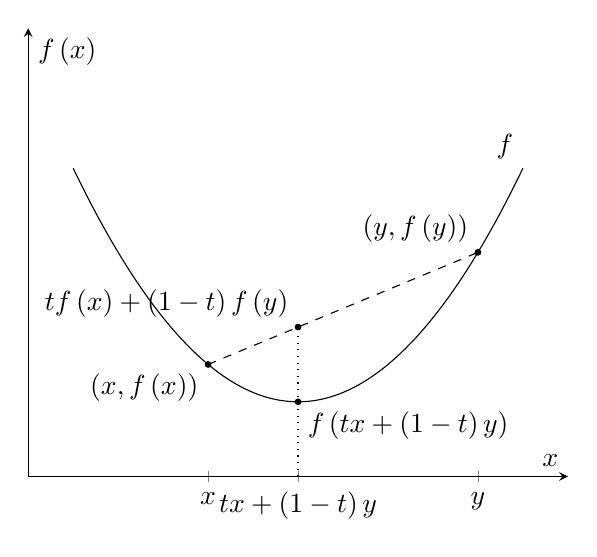
\begin{tikzpicture}
        \begin{axis}[
            axis lines = middle,
            xlabel = {\(x\)},
            ylabel = {\(f\pqty{x}\)},
            xmin = 0, xmax = 6,
            ymin = 0, ymax = 6,
            samples = 100,
            domain = 0.5:5.5,
            xtick = {2, 3, 5},
            xticklabels = {\(x\), \(tx+\pqty{1-t}y\), \(y\)},
            ytick = \empty
        ]

            \addplot[no marks] {0.5*(x-3)^2 + 1};
            \node[above left] at (axis cs:5.5,4.125) {\(f\)};

            \addplot[only marks, mark=*, mark size=1pt]
                coordinates {(2, 1.5) (5, 3)};

            \node[below left] at (axis cs:2, 1.5) {\(\pqty{x, f\pqty{x}}\)};
            \node[above left] at (axis cs:5, 3) {\(\pqty{y, f\pqty{y}}\)};

            \addplot[dashed] coordinates {(2, 1.5) (5, 3)};
            \addplot[only marks, mark=*, mark size=1pt]
                coordinates {(3, 2) (3, 1)};
            \node[above left] at (axis cs:3, 2) {\(t f\pqty{x} + \pqty{1 - t} f\pqty{y}\)};
            \node[below right] at (axis cs:3, 1) {\(f\pqty{tx + \pqty{1 - t} y}\)};

            \addplot[dotted] coordinates {(3, 0) (3, 2)};

        \end{axis}
    \end{tikzpicture}

    \caption{Convex Function}
    \label{probability-fig:convex-fn}
\end{figure}

The definition is illustrated in \autoref{probability-fig:convex-fn}.

\begin{theorem}[Jensen's Inequality]\label{probability-theorem-008}
    \label{probability-thm:jensen}%
Assume \(\Expt[|X|]<\infty\). The convex finite-valued function \(f\) has an affine lower bound, so \(\Expt[f(X)]\) is well-defined, possibly \(+\infty\).
    Let \(X\) be a random variable, and \(\functiondomain{f}{\RR}{\RR}\) be a convex function. Then
    \[
        \Expt\bqty{f\pqty{X}} \geq f\pqty{\Expt\bqty{X}}.
    \]
\end{theorem}

\begin{figure}[ht!]
    \centering
    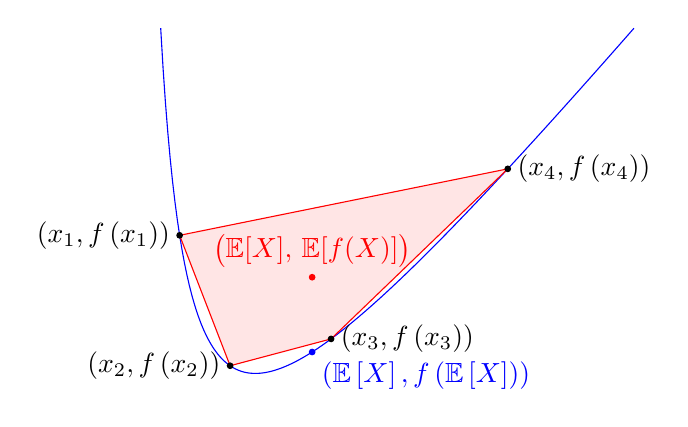
\begin{tikzpicture}
        \begin{axis}[
            axis lines = none,
            xmin = -2, xmax = 4.5,
            ymin = 0, ymax = 4.5,
            samples = 200,
            domain = 0.25:4,
            width = 12cm
        ]

        \addplot[no marks, blue]{1 / x + x};

        \pgfmathsetmacro{\xa}{0.4}
        \pgfmathsetmacro{\xb}{0.8}
        \pgfmathsetmacro{\xc}{1.6}
        \pgfmathsetmacro{\xd}{3}
        \pgfmathsetmacro{\xe}{(\xa + \xb + \xc + \xd) / 4}

        \pgfmathsetmacro{\fa}{1 / \xa + \xa}
        \pgfmathsetmacro{\fb}{1 / \xb + \xb}
        \pgfmathsetmacro{\fc}{1 / \xc + \xc}
        \pgfmathsetmacro{\fd}{1 / \xd + \xd}
        \pgfmathsetmacro{\fe}{1 / \xe + \xe}

        \pgfmathsetmacro{\ef}{(\fa + \fb + \fc + \fd) / 4}

        \addplot[only marks, mark=*, mark size=1pt]
                coordinates {(\xa, \fa) (\xb, \fb) (\xc, \fc) (\xd, \fd)};

        \node[left] at (axis cs:\xa, \fa) {\(\pqty{x_1, f\pqty{x_1}}\)};
        \node[left] at (axis cs:\xb, \fb) {\(\pqty{x_2, f\pqty{x_2}}\)};
        \node[right] at (axis cs:\xc, \fc) {\(\pqty{x_3, f\pqty{x_3}}\)};
        \node[right] at (axis cs:\xd, \fd) {\(\pqty{x_4, f\pqty{x_4}}\)};

        \addplot[
            fill=red!10,
            draw=red
        ]
        coordinates {
            (\xa, \fa)
            (\xb, \fb)
            (\xc, \fc)
            (\xd, \fd)
            (\xa, \fa)
        };

        \addplot[only marks, mark=*, mark size=1pt, blue]
            coordinates {(\xe,\fe)};
        \node[blue, below right] at (axis cs:\xe, \fe) {\(\pqty{\Expt\bqty{X}, f\pqty{\Expt\bqty{X}}}\)};

        % (E[X], E[f(X)]) point
        \addplot[only marks, mark=*, mark size=1pt, red]
            coordinates {(\xe,\ef)};

        \node[red, above] at (axis cs:\xe,\ef)
            {$\bigl(\mathbb E[X],\,\mathbb E[f(X)]\bigr)$};
        \end{axis}
    \end{tikzpicture}

    \caption{Jensen's Inequality}
    \label{probability-fig:jensen-inequality}
\end{figure}

A trick to remembering the direction of the inequality is that since
\[
    \Var\pqty{X} = \Expt\bqty{\pqty{X - \Expt\bqty{X}}^2} \geq 0
\]
and also
\[
    \Var\pqty{X} = \Expt\bqty{X^2} - \Expt\bqty{X}^2,
\]
and note \(f\pqty{x} = x^2\) is convex and
\[
    \Expt\bqty{X^2} \geq \pqty{\Expt\bqty{X}}^2.
\]

To visualise \autoref{probability-thm:jensen} (Jensen's Inequality), \autoref{probability-fig:jensen-inequality} considers a uniform distribution over \(\Bqty{x_1, x_2, x_3, x_4}\), and the centre of the quadrilateral is marked red, with \(y\)-coordinate \(\Expt\bqty{f\pqty{X}}\), while \(f\pqty{\Expt\bqty{X}}\) is marked as the blue dot on the curve.

The same supporting-line proof works for a finite convex function on any open interval containing the values of the integrable variable and its mean. We first produce useful lemmas for the proof.

\begin{lemma}[Convex Function lies above Tangents]\label{probability-lemma-007}
    \label{probability-lem:convex-fn-tangents}%
    A convex function \(\functiondomain{f}{\RR}{\RR}\) is the supremum of all the lines lying below it. In other words,
    \[
        \forall m \in \RR, \exists a, b \in \RR: f\pqty{m} = am + b \land \forall x \in \RR: f\pqty{x} \geq ax + b.
    \]
\end{lemma}

\begin{figure}[ht!]
    \centering
    \begin{tikzpicture}
        \begin{axis}[
            axis lines = middle,
            xlabel = {\(x\)},
            ylabel = {\(f(x)\)},
            xmin = -1, xmax = 5,
            ymin = -2, ymax = 9,
            xtick = \empty,
            ytick = \empty,
            domain = 0:4,
            samples = 100,
            width = 10cm
        ]

            \addplot[no marks, thick, blue] {0.5*x^2};

            \addplot[only marks, mark=*, mark size = 1pt] coordinates {(1, 0.5) (2, 2) (3, 4.5)};

            \addplot[domain=0.25:4.5] {1 * (x - 1) + 0.5};
            \addplot[domain=0.4:4.2] {2 * (x - 2) + 2};
            \addplot[domain=0.5:4.1] {3 * (x - 3) + 4.5};
        \end{axis}
    \end{tikzpicture}

    \caption{Convex Function and its Tangents}
    \label{probability-fig:convex-fn-tangents}
\end{figure}

\autoref{probability-fig:convex-fn-tangents} visualises this.

\begin{proof}\label{probability-proof-030}
    Let \(m \in \RR\) and \(x < m < y\). Then
    \[
        m = tx + \pqty{1 - t}y
    \]
    for some \(t \in \oointv{0}{1}\). This gives
    \[
        t\pqty{m - x} = \pqty{1 - t} \pqty{y - m}.
    \]

    By convexity,
    \[
        f\pqty{m} = f\pqty{tx + \pqty{1 - t} y} \leq t f\pqty{x} + \pqty{1 - t} f\pqty{y}
    \]
    and hence
    \[
        t\pqty{f\pqty{m} - f\pqty{x}} \leq \pqty{1 - t} \pqty{f\pqty{y} - f\pqty{m}}.
    \]

    Hence,
    \[
        \frac{f\pqty{m} - f\pqty{x}}{m - x} \leq \frac{f\pqty{y} - f\pqty{m}}{y - m}.
    \]

    Let
    \[
        a = \sup_{x < m} \frac{f\pqty{m} - f\pqty{x}}{m - x}.
    \]

    Then, from the previous inequality on the gradients,
    \[
        \frac{f\pqty{m} - f\pqty{x}}{m - x} \leq a \leq \frac{f\pqty{y} - f\pqty{m}}{y - m}.
    \]

    So this gives that
    \[
        f\pqty{z} \geq a\pqty{z - m} + f\pqty{m},
    \]
    for all \(z \in \RR\), with the equal sign taking place if \(z = m\).
\end{proof}

Now we use \autoref{probability-lem:convex-fn-tangents} to prove \autoref{probability-thm:jensen} (Jensen's Inequality).

\begin{proof}[\proofname\ of \autoref{probability-thm:jensen} (Jensen's Inequality)]\label{probability-proof-031}
    Let \(m = \Expt\bqty{X}\). By the claim, there is some \(a, b \in \RR\), such that
    \[
        f\pqty{m} = am + b
    \]
    and
    \[
        f\pqty{x} \geq ax + b
    \]
    for all \(x\). Then, we have
    \[
        f\pqty{X} \geq aX + b.
    \]

    Taking expectations on both sides, we get
    \[
        \Expt\bqty{f\pqty{X}} \geq a \Expt\bqty{X} + b = am + b = f\pqty{m} = f\pqty{\Expt\bqty{X}}.
    \]
\end{proof}

Similar to when we study Cauchy--Schwarz back then, we study the cases of equality.

Let \(\functiondomain{f}{\RR}{\RR}\) be convex, and with the extra property that for \(m = \Expt\bqty{X}\), there is some \(a, b \in \RR\), such that
\[
    f\pqty{m} = am + b \land \forall x \in \RR \setminus \Bqty{m}: f\pqty{x} > ax + b,
\]
i.e. let \(f\) be strictly convex at \(m\). Note that 
\[
    f\pqty{X} - \pqty{aX + b} \geq 0.
\]

Taking expectation on both sides, we have
\[
    \Expt\bqty{f\pqty{X}} \geq a \Expt\bqty{X} + b = am + b = f\pqty{m} = f\pqty{\Expt\bqty{X}}.
\]

We want that \(\Expt\bqty{f\pqty{X}} = f\pqty{\Expt\bqty{X}}\), so this forces
\[
    \Expt\bqty{f\pqty{X} - \pqty{aX + b}} = 0
\]
which implies that
\[
    \Prob\pqty{f\pqty{X} = aX + b} = 1.
\]

But this now forces \(X = m\), so \(\Prob\pqty{X = m} = 1\).

There is a nice result due to Jensen's Inequality.

\begin{theorem}[Finite Jensen Inequality]\label{probability-theorem-009}
    \label{probability-thm:am-gm}
    Let \(f:I\to\RR\) be convex on an open interval \(I\). Then for all \(x_1, \ldots, x_n \in I\), we have
    \[
        \frac{1}{n} \sum_{k = 1}^{n} f\pqty{x_k} \geq f\pqty{\frac{\sum_{k = 1}^{n} x_k}{n}}.
    \]
\end{theorem}

\begin{proof}\label{probability-proof-032}
    Let \(I\) be uniform on \(\{1,\ldots,n\}\), and set \(X=x_I\). This also covers repeated values among the \(x_i\).

    Hence,
    \[
        \frac{1}{n} \sum_{k = 1}^{n} f\pqty{x_k} = \Expt\bqty{f\pqty{X}} = \sum_{x \in \RR} f\pqty{x} \Prob\pqty{X = x}.
    \]

    By \autoref{probability-thm:jensen} (Jensen's Inequality), we have
    \[
        \Expt\bqty{f\pqty{X}} \geq f\pqty{\Expt\bqty{X}} = f\pqty{\frac{\sum_{k = 1}^{n} x_k}{n}}.
    \]
\end{proof}

\begin{remark}\label{probability-remark-005}
    The more commonly seen AM--GM inequality is a corollary of this. Let \(f\pqty{x} = - \log x\), for \(x > 0\). Take \(x_1, \ldots, x_n > 0\), we have
    \[
        - \frac{1}{n} \sum_{k = 1}^{n} \log x_k \geq - \log \pqty{\frac{\sum_{k = 1}^{n} x_k}{n}}.
    \]

    Exponentiating both sides, we get
    \[
        \pqty{\prod_{k = 1}^{n} x_k}^{\frac{1}{n}} \leq \frac{1}{n} \sum_{k = 1}^{n} x_k.
    \]
\end{remark}

\section{Joint Distribution}\label{probability-section-07}
In this section variables are discrete. For conditional expectations, assume
\(X\) and each variable whose expectation is taken are integrable, unless
non-negativity is explicitly allowed. Sums over \(y\) in conditional formulas
range over \(\{y:\Prob(Y=y)>0\}\). Values of a conditional expectation on
null events may be assigned arbitrarily; identities hold almost surely.


Recall that, if \(X\) is a discrete random variable then the distribution of \(X\) is \(\pqty{\Prob\pqty{X = x}}_x\).

\subsection{Joint Distribution}

\begin{definition}[Joint Distribution for Discrete Variables]\label{probability-definition-031}
    \label{probability-def:joint-distribution-discrete}%
    Let \(X_1, \ldots, X_n\) be discrete random variables. Their \emph{joint distribution} is defined to be
    \[
        \Prob\pqty{X_1 = x_1, \ldots, X_n = x_n}
    \]
    for all possible values of \(x_1, x_2, \ldots, x_n\).
\end{definition}

Note that we could recover the individual distribution of a single random variable from this as well. Indeed, we have
\[
    \Prob\pqty{X_1 = x_1} = \sum_{x_2, \ldots, x_n \in \RR} \Prob\pqty{X_1 = x_1, \ldots, X_n = x_n}
\]
where we note that this sum is countable since \(x_i\)s only take countably many values. We call this the \emph{marginal distribution} of \(X_1\).

\begin{definition}[Conditional Distribution for Discrete Variables]\label{probability-definition-032}
    \label{probability-def:conditional-distribution-discrete}%
    Let \(X\) and \(Y\) be two discrete random variables. The \emph{conditional distribution} of \(X\), given \(Y = y\) (where \(y\) is fixed and \(\Prob(Y=y)>0\)) is defined to be
    \[
        \Prob\pqty{\Conditional{X = x}{Y = y}} = \frac{\Prob\pqty{X = x, Y = y}}{\Prob\pqty{Y = y}}
    \]
    for all possible values of \(x\).
\end{definition}

By \autoref{probability-thm:law-total-probability} (Law of Total Probability), we have
\[
    \Prob\pqty{X = x} = \sum_{y \in \RR} \Prob\pqty{\Conditional{X = x}{Y = y}} \cdot \Prob\pqty{Y = y}
\]
noting that this sum is similarly countable.

\subsection{Sum of Random Variables}

\begin{example}[Distribution of Sum of Random Variables]\label{probability-example-025}
    \label{probability-ex:distribution-sum-discrete}%
    Let \(X\) and \(Y\) be two independent random variables. We want to understand the distribution of \(X + Y\). We have
    \begin{align*}
        \Prob\pqty{X + Y = z} &= \sum_{y \in \RR} \Prob\pqty{X + Y = z, Y = y} \\
        &= \sum_{y \in \RR} \Prob\pqty{X = z - y, Y = y} \\
        &= \sum_{y \in \RR} \Prob\pqty{X = z - y} \cdot \Prob\pqty{Y = y}.
    \end{align*}
\end{example}

\begin{definition}[Convolution of Distribution for Discrete Variables]\label{probability-definition-033}
    \label{probability-def:convolution-distribution-discrete}%
    Let \(X, Y\) be two independent discrete random variables. Then the distribution of \(X + Y\), given by
    \[
        \sum_{y \in \RR} \Prob\pqty{X = z - y} \cdot \Prob\pqty{Y = y}
    \]
    is the \emph{convolution} of their probability laws (represented here by their mass functions or densities).
\end{definition}

\begin{example}[Sum of Poisson Random Variables]\label{probability-example-026}
    Let \(X \sim \Poisson\pqty{\lambda}\), \(Y \sim \Poisson\pqty{\mu}\), \(\lambda, \mu > 0\) and \(X \indp Y\). We may show that the sum of two independent Poisson random variables is another Poisson random variable.

    \begin{align*}
        \Prob\pqty{X + Y = n} &= \sum_{k = 0}^{n} \Prob\pqty{X = n - k} \cdot \Prob\pqty{Y = k} \\
        &= \sum_{k = 0}^{n} e^{-\lambda} \cdot \frac{\lambda^{n - k}}{\pqty{n - k}!} \cdot e^{-\mu} \cdot \frac{\mu^k}{k!} \\
        &= \frac{e^{-\pqty{\lambda + \mu}}}{n!} \cdot \sum_{k = 0}^{n} \binom{n}{k} \cdot \lambda^{n - k} \cdot \mu^k \\
        &= e^{-\pqty{\lambda + \mu}} \cdot \frac{\pqty{\lambda + \mu}^n}{n!}.
    \end{align*}

    Therefore, we have
    \[
        \Prob\pqty{X + Y = n} = e^{-\pqty{\lambda + \mu}} \cdot \frac{\pqty{\lambda + \mu}^n}{n!}
    \]
    and hence
    \[
        X + Y \sim \Poisson \pqty{\lambda + \mu}.
    \]

    Indeed, if \(\lambda = \mu\), let \(X_n, Y_n \sim \Binomial\pqty{n, \frac{\lambda}{n}}\) and \(X_n \indp Y_n\). We know a Poisson distribution is a limit of binomial random variables, and indeed
    \[
        X_n + Y_n \sim \Binomial\pqty{2n, \frac{\lambda}{n}}.
    \]
\end{example}

\subsection{Conditional Expectation}

\begin{definition}[Conditonal Expectation upon an Event]\label{probability-definition-034}
    \label{probability-def:conditional-expectation-upon-event}
Assume \(X\) is integrable; any conditioning variable here is discrete. Conditional equalities hold almost surely.
%
    The \emph{conditional expectation} of a random variable \(X\) with respect to an event \(B\), where \(\Prob\pqty{B} > 0\), is given by
    \[
        \Expt\bqty{\Conditional{X}{B}} = \frac{\Expt\bqty{X \cdot \indicator\pqty{B}}}{\Prob\pqty{B}}.
    \]
\end{definition}

Note that with \(X = \indicator\pqty{A}\), we do recover consistent definitions with conditional probability of events.

\[
    \Expt\bqty{\Conditional{\indicator\pqty{A}}{B}} = \frac{\Expt\bqty{\indicator\pqty{A} \cdot \indicator\pqty{B}}}{\Prob\pqty{B}} = \frac{\Expt\bqty{\indicator\pqty{A \cap B}}}{\Prob\pqty{B}} = \frac{\Prob\pqty{A \cap B}}{\Prob\pqty{B}} = \Prob\pqty{\Conditional{A}{B}}.
\]

\begin{theorem}[Law of Total Expectation]\label{probability-theorem-010}
    \label{probability-thm:law-of-total-expectation}
Assume \(X\) is integrable; any conditioning variable here is discrete. Conditional equalities hold almost surely.
%
    Let \(X\) be a random variable, \(\pqty{\Omega_i}\) be a partition of \(\Omega\) into disjoint sets, with \(\Prob\pqty{\Omega_i} > 0\) for all \(i = 1, 2, \ldots ,n\). Then we have
    \[
        \Expt\bqty{X} = \sum_{i = 1}^{n} \Expt\bqty{\Conditional{X}{\Omega_i}} \cdot \Prob\pqty{\Omega_i}.
    \]
\end{theorem}

\begin{proof}\label{probability-proof-033}
    We have
    \begin{align*}
        \Expt\bqty{X} &= \Expt\bqty{X \cdot \indicator\pqty{\Omega}} \\
        &= \Expt\bqty{X \cdot \sum_{i = 1}^{n} \indicator \pqty{\Omega_i}} \\
        &= \sum_{i = 1}^{n} \Expt\bqty{X \cdot \indicator \pqty{\Omega_i}} \\
        &= \sum_{i = 1}^{n} \Expt\bqty{\Conditional{X}{\Omega_i}} \cdot \Prob\pqty{\Omega_i}
    \end{align*}
\end{proof}

The conditional expectation of \(X\) given \(Y = y\) is defined similarly, since \(Y = y\) is an event:
\[
    \Expt\bqty{\Conditional{X}{Y = y}} = \frac{\Expt\bqty{X \cdot \indicator\pqty{Y = y}}}{\Prob\pqty{Y = y}}.
\]

\begin{proposition}[Conditional Expectation upon Random Variable Event]\label{probability-proposition-017}
    \label{probability-prop:conditional-expectation-random-variable}
For the pointwise formula require \(\Prob(Y=y)>0\).

Assume \(X\) is integrable; any conditioning variable here is discrete. Conditional equalities hold almost surely.
%
    We have
    \[
        \Expt\bqty{\Conditional{X}{Y = y}} = \sum_{x \in \RR} x \cdot \Prob\pqty{\Conditional{X = x}{Y = y}}.
    \]
\end{proposition}

\begin{proof}\label{probability-proof-034}
    We have
    \begin{align*}
        \Expt\bqty{\Conditional{X}{Y = y}} &= \frac{\Expt\bqty{X \cdot \indicator\pqty{Y = y}}}{\Prob\pqty{Y = y}} \\
        &= \sum_{x \in \RR} x \cdot \frac{\Prob\pqty{X = x, Y = y}}{\Prob\pqty{Y = y}} \\
        &= \sum_{x \in \RR} x \cdot \Prob\pqty{\Conditional{X = x}{Y = y}}.
    \end{align*}
\end{proof}

This shows that the conditional expectation is consistent with the expectation of the conditional random variable.

\begin{definition}[Conditional Expectation Distribution]\label{probability-definition-035}
    \label{probability-def:conditional-expectation-distribution}
Set \(g(y)=0\) whenever \(\Prob(Y=y)=0\); any other assignment there gives the same almost-sure random variable.

Assume \(X\) is integrable; any conditioning variable here is discrete. Conditional equalities hold almost surely.
%
    We define \(\Expt\bqty{\Conditional{X}{Y}}\) as a random variable as
    \[
        \Expt\bqty{\Conditional{X}{Y}} = g\pqty{Y} = \sum_{y \in \RR} g\pqty{y} \cdot \indicator\pqty{Y = y},
    \]
    where
    \[
        g\pqty{y} = \Expt\bqty{\Conditional{X}{Y = y}}.
    \]
\end{definition}

This notation may seem confusing at the start. For example, if \(g\pqty{y} = y^2\), we have
\[
    \Expt\bqty{\Conditional{X}{Y}} = g\pqty{Y} = Y^2.
\]

Intuitively, this is the \textbf{best approximation in mean squared error when \(X\) has finite second moment} of \(X\) using the random variable \(Y\). In the two extreme cases, if \(X = f\pqty{Y}\), then we have
\[
    \Expt\bqty{\Conditional{X}{Y}} = f\pqty{Y},
\]
and if \(X \indp Y\), we have
\[
    \Expt\bqty{\Conditional{X}{Y}} = \Expt\bqty{X}.
\]

As a function, we may define it for \(\omega \in \Omega\),
\[
    \Expt\bqty{\Conditional{X}{Y}}\pqty{\omega} = \Expt\bqty{\Conditional{X}{Y = Y\pqty{\omega}}}.
\]

\begin{example}[Conditional Expectation for Tossing \(p\)-Coin]\label{probability-example-027}
    \label{probability-ex:conditional-expectatio-tossing-p-coin}%
For the displayed binomial-ratio calculation assume \(0<p<1\) and \(1\le y\le n\); at \(y=0\) the conditional mean is zero. The resulting almost-sure identity also holds at \(p=0,1\) by determinism.
    Toss a \(p\)-coin independently for \(n\) times. Let \(X_i\) be the indicator that the \(i\)th toss is a head, for \(i = 1, 2, \ldots, n\), and let \(Y_n = X_1 + X_2 + \cdots + X_n\).

    We set \(g\pqty{y} = \Expt\bqty{\Conditional{X_1}{Y_n = y}}\). Note that
    \begin{align*}
        g\pqty{y} &= \Expt\bqty{\Conditional{X_1}{Y_n = y}} \\
        &= \frac{\Expt\bqty{X_1 \cdot \indicator\pqty{Y_n = y}}}{\Prob\pqty{Y_n = y}} \\
        &= \frac{\Prob\pqty{X_1 = 1, Y_n = y}}{\Prob\pqty{Y_n = y}} \\
        &= \frac{p \cdot \binom{n - 1}{y - 1} \cdot p^{y - 1} \cdot \pqty{1 - p}^{n - y}}{\binom{n}{y} \cdot p^y \cdot \pqty{1 - p}^{n - y}} \\
        &= \frac{y}{n}.
    \end{align*}

    Hence,
    \[
        \Expt\bqty{\Conditional{X_1}{Y_n}} = \frac{Y_n}{n}.
    \]

    Indeed, this makes sense, since one would probably expect each \(X_i\) to be \(\frac{Y}{n}\) `on average'.
\end{example}

\begin{proposition}[Properties of Conditional Expectation Distribution]\label{probability-proposition-018}
    \label{probability-prop:conditional-expectation-distribution-property}
All variables inside a conditional expectation are integrable.
%
    For any \(c \in \RR\), we have
    \begin{itemize}
        \item \(\Expt\bqty{\Conditional{cX}{Y}} = c \Expt\bqty{\Conditional{X}{Y}}\).
        \item \(\Expt\bqty{\Conditional{c + X}{Y}} = c + \Expt\bqty{\Conditional{X}{Y}}\) and \(\Expt\bqty{\Conditional{c}{Y}} = c\).
        \item If \(X_1, X_2, \ldots, X_n\) and \(Y\) are random variables, then we have
        \[
            \Expt\bqty{\Conditional{\sum_{i = 1}^{n} X_i}{Y}} = \sum_{i = 1}^{n} \Expt\bqty{\Conditional{X_i}{Y}}.
        \]
    \end{itemize}
\end{proposition}

\begin{proposition}[Expectation of Conditional Expectation Distribution]\label{probability-proposition-019}
    \label{probability-prop:expectation-conditional-expectation-distribution}
Assume \(X\) is integrable; any conditioning variable here is discrete. Conditional equalities hold almost surely.
%
    We have
    \[
        \Expt\bqty{\Expt\bqty{\Conditional{X}{Y}}} = \Expt\bqty{X}.
    \]
\end{proposition}

\begin{proof}\label{probability-proof-035}
    Recall that
    \[
        \Expt\bqty{\Conditional{X}{Y}} = \sum_{y \in \RR} \indicator\pqty{Y = y} \Expt\bqty{\Conditional{X}{Y = y}}.
    \]

    Taking the expectations on both sides, we have
    \[
        \Expt\bqty{\Expt\bqty{\Conditional{X}{Y}}} = \sum_{y \in \RR} \Prob\pqty{Y = y} \cdot \Expt\bqty{\Conditional{X}{Y = y}} = \Expt\bqty{X}.
    \]
\end{proof}

\begin{proposition}[Conditional Expectation Distribution of Independent Variables]\label{probability-proposition-020}
    \label{probability-prop:conditional-expectation-distribution-independent}
Assume \(X\) is integrable; any conditioning variable here is discrete. Conditional equalities hold almost surely.
%
    Let \(X\) and \(Y\) be independent. Then
    \[
        \Expt\bqty{\Conditional{X}{Y}} = \Expt\bqty{X}.
    \]
\end{proposition}

\begin{proof}\label{probability-proof-036}
    Recall that by definition,
    \begin{align*}
        \Expt\bqty{\Conditional{X}{Y = y}} &= \sum_{x \in \RR} x \cdot \Prob\pqty{\Conditional{X = x}{Y = y}} \\
        &= \sum_{x \in \RR} x \cdot \Prob\pqty{X = x} \\
        &= \Expt\bqty{X}.
    \end{align*}

    Hence,
    \[
        \Expt\bqty{\Conditional{X}{Y}} = \Expt\bqty{X} \sum_{y \in \RR} \indicator\pqty{Y = y} = \Expt\bqty{X}
    \]
    as desired.
\end{proof}

\begin{proposition}[Conditional Expectation upon Independent Conditions]\label{probability-proposition-021}
    \label{probability-prop:conditional-expectation-independent-conditions}
Assume also that \(Y\) and \(Z\) are discrete.

Assume \(X\) is integrable; any conditioning variable here is discrete. Conditional equalities hold almost surely.
%
    Let \(Y\) and \(Z\) be two independent random variables. Then
    \[
        \Expt\bqty{\Conditional{\Expt\bqty{\Conditional{X}{Y}}}{Z}} = \Expt\bqty{X}.
    \]
\end{proposition}

\begin{proof}\label{probability-proof-037}
    Set \(g\pqty{Y} = \Expt\bqty{\Conditional{X}{Y}}\), while \(g\pqty{y} = \Expt\bqty{\Conditional{X}{Y = y}}\).

    First, we claim that \(g\pqty{Y}\) is independent of \(Z\). We want to show that for all \(w, z\), we have
    \[
        \Prob\pqty{g\pqty{Y} = w, Z = z} = \Prob\pqty{g\pqty{Y} = w} \cdot \Prob\pqty{Z = z}.
    \]

    We have
    \begin{align*}
        \Prob\pqty{g\pqty{Y} = w, Z = z} &= \sum_{y \in g\inverse\pqty{\Bqty{w}}} \Prob\pqty{Y = y, Z = z} \\
        &= \sum_{y \in g\inverse\pqty{\Bqty{w}}} \Prob\pqty{Y = y} \cdot \Prob\pqty{Z = z} \\
        &= \Prob\pqty{Z = z} \cdot \sum_{y \in g\inverse\pqty{\Bqty{w}}} \Prob\pqty{Y = y} \\
        &= \Prob\pqty{Z = z} \cdot \Prob\pqty{g\pqty{Y} = w}.
    \end{align*}

    Therefore, \(g\pqty{Y} \indp Z\).

    Therefore, by \autoref{probability-prop:conditional-expectation-distribution-independent} we have
    \[
        \Expt\bqty{\Conditional{\Expt\bqty{\Conditional{X}{Y}}}{Z}} = \Expt\bqty{\Conditional{g\pqty{Y}}{Z}} = \Expt\bqty{g\pqty{Y}},
    \]
    and we have from \autoref{probability-prop:expectation-conditional-expectation-distribution},
    \[
        \Expt\bqty{g\pqty{Y}} = \Expt\bqty{\Expt\bqty{\Conditional{X}{Y}}} = \Expt\bqty{X}.
    \]
\end{proof}

\begin{proposition}[Extraction of Function of Condition]\label{probability-proposition-022}
    \label{probability-prop:extraction-function-condition}%
Assume \(X\) and \(h(Y)X\) are integrable (bounded \(h\) suffices).
    For any function \(\functiondomain{h}{\RR}{\RR}\), we have
    \[
        \Expt\bqty{\Conditional{h\pqty{Y} \cdot X}{Y}} = h\pqty{Y} \cdot \Expt\bqty{\Conditional{X}{Y}}.
    \]
\end{proposition}

\begin{proof}\label{probability-proof-038}
    We have
    \begin{align*}
        \Expt\bqty{\Conditional{h\pqty{Y} \cdot X}{Y}} &= \sum_{y \in \RR} \indicator\pqty{Y = y} \cdot \Expt\bqty{\Conditional{h\pqty{Y} \cdot X}{Y = y}} \\
        &= \sum_{y \in \RR} \indicator\pqty{Y = y} \cdot h\pqty{Y} \cdot \Expt\bqty{\Conditional{X}{Y = y}} \\
        &= h\pqty{Y} \cdot \sum_{y \in \RR} \indicator\pqty{Y = y} \cdot \Expt\bqty{\Conditional{X}{Y = y}} \\
        &= h\pqty{Y} \cdot \Expt\bqty{\Conditional{X}{Y}}.
    \end{align*}
\end{proof}

We have two corollaries due to the properties above.

\begin{corollary}[Conditional Expectation upon Same Condition]\label{probability-corollary-005}
    \label{probability-cor:conditional-expecation-upon-same-condition}
Assume \(X\) is integrable; any conditioning variable here is discrete. Conditional equalities hold almost surely.
%
    We have
    \[
        \Expt\bqty{\Conditional{\Expt\bqty{\Conditional{X}{Y}}}{Y}} = \Expt\bqty{\Conditional{X}{Y}}.
    \]
\end{corollary}

\begin{corollary}[Conditional Expectation upon Itself]\label{probability-corollary-006}
    \label{probability-cor:conditional-expectation-upon-itself}
Assume \(X\) is integrable; any conditioning variable here is discrete. Conditional equalities hold almost surely.
%
    We have
    \[
        \Expt\bqty{\Conditional{X}{X}} = X.
    \]    
\end{corollary}

\begin{example}[Conditional Expectation for Tossing \(p\)-Coin, Revisited]\label{probability-example-028}
    \label{probability-ex:conditional-expectatio-tossing-p-coin-revisited}%
    We revisit \autoref{probability-ex:conditional-expectatio-tossing-p-coin}. We toss a \(p\)-coin \(n\) times independently. Let \(X_i = \indicator\pqty{i\text{-th toss is H}}\) for \(i = 1, 2, \ldots, n\), and let
    \[
        Y_n = X_1 + \cdots + X_n.
    \]

    By symmetry, for all \(i = 1, 2, \ldots, n\), we have
    \[
        \Expt\bqty{\Conditional{X_i}{Y_n}} = \Expt\bqty{\Conditional{X_1}{Y_n}}
    \]

    Note that
    \[
        \Expt\bqty{\Conditional{\sum_{i = 1}^{n} X_i}{Y_n}} = \Expt\bqty{\Conditional{Y_n}{Y_n}} = Y_n,
    \]
    while using linearity gives
    \[
        \Expt\bqty{\Conditional{\sum_{i = 1}^{n} X_i}{Y_n}} = \sum_{i = 1}^{n} \Expt\bqty{\Conditional{X_i}{Y_n}} = n \cdot \Expt\bqty{\Conditional{X_1}{Y_n}}.
    \]

    Hence,
    \[
        \Expt\bqty{\Conditional{X_1}{Y_n}} = \frac{Y_n}{n}.
    \]
\end{example}
\begin{proposition}[Conditional mean as least-squares predictor]\label{probability-proposition-023}
For square-integrable \(X\) and discrete \(Y\), set \(g(Y)=\Expt[X\mid Y]\).
For every square-integrable function \(h(Y)\),
\[\Expt[(X-h(Y))^2]=\Expt[(X-g(Y))^2]+\Expt[(g(Y)-h(Y))^2].\]
Thus \(g(Y)\) uniquely minimises mean squared error, up to almost-sure equality.
\end{proposition}
\begin{proof}\label{probability-proof-039}
Conditional Cauchy--Schwarz on each event \(\{Y=y\}\) gives
\(g(y)^2\le\Expt[X^2\mid Y=y]\), so \(g(Y)\) is square-integrable.
Expand the square with \(X-h=(X-g)+(g-h)\). The cross term vanishes since
\(\Expt[X-g(Y)\mid Y]=0\) and \(g-h\) is a function of \(Y\).
\end{proof}


\section{Random Walk}\label{probability-section-08}

\begin{definition}[Random/Stochastic Process]\label{probability-definition-036}
    \label{probability-def:random-stochastic-process}%
    A discrete-time \emph{random/stochastic process} is a sequence of random variables \(\pqty{X_n}_{n \in \NN}\).
\end{definition}

\begin{definition}[Random Walk]\label{probability-definition-037}
    \label{probability-def:random-walk}%
    A \emph{random walk} is a random process that can be expressed in the following way:
    \[
        X_n = x + \sum_{i = 1}^{n} Y_i,
    \]
    where \(x\) is a deterministic number, and \(\pqty{Y_i}_{i \in \NN}\)s are independent and identically distributed (i.i.d.). The random variables \(Y_i\)s the \emph{steps} of the random walk.
\end{definition}

\begin{definition}[Simple Random Walk]\label{probability-definition-038}
    \label{probability-def:simple-random-walk}%
    A random walk is \emph{simple} if the steps can only take values \(\pm 1\).
\end{definition}

In this case, we may set \(\Prob\pqty{Y_i = 1} = p\) and \(\Prob\pqty{Y_i = -1} = q\), with \(p + q = 1\) and \(p, q \geq 0\).

\begin{notation}\label{probability-notation-002}
    \(\Prob_x\) denotes the law of the walk started deterministically at \(x\), and \(\Expt_x\) its expectation. This does not require conditioning a single reference law on a possibly null event.
\end{notation}

\begin{example}[Gambler's Ruin Estimates]\label{probability-example-029}
    \label{probability-ex:gambler-ruin-estimates}%
Assume \(a\in\NN\), \(a\ge2\), \(x\in\{0,\ldots,a\}\), and \(0<p<1\).
    We may think of \(\pqty{X_n}\) as the fortune of a gambler, who starts with \(x\) in their pocket at time \(0\), and every time step they bet \(1\), which he loses with probability \(\pqty{1 - p}\), and gets it back doubled with probability \(p\). The game ends if they reach \(0\) (which means they go bankrupt) or they reach \(a\), whichever happens first.

    We want to know the probability they reach \(a\) before going bankrupt. We let
    \[
        h\pqty{x} = \Prob_x \pqty{\pqty{X_n} \text{ reaches }a\text{ before reaching }0}.
    \]

    Note that \(h\pqty{0} = 0\) and \(h\pqty{a} = 1\). We have
    \begin{align*}
        h\pqty{x} &= \Prob_x \pqty{X \text{ reaches }a\text{ before }0} \\
        &= \Prob_x \pqty{\Conditional{X \text{ reaches }a\text{ before }0}{Y_1 = 1}} \cdot p + \Prob_x \pqty{\Conditional{X \text{ reaches }a\text{ before }0}{Y_1 = -1}} \cdot \pqty{1 - p} \\
        &= p \cdot h \pqty{x + 1} + \pqty{1 - p} \cdot h \pqty{x - 1}.
    \end{align*}

    We now consider particular cases of \(p\) and \(q\).

    \begin{itemize}
        \item If \(p = q = \frac{1}{2}\), this is called \emph{simple symmetric random walk}, and the system reduces to \(h\pqty{x} = \frac{1}{2} h \pqty{x + 1} + \frac{1}{2} h \pqty{x - 1}\).
        
        Notice that simplifying this gives
        \[
            h\pqty{x + 1} - h\pqty{x} = h\pqty{x} - h\pqty{x - 1} = \cdots = c.
        \]

        Therefore, we have \(h\pqty{x} = \sum_{i = 1}^{x} \pqty{h\pqty{i} - h\pqty{i - 1}} = cx\). Since \(h\pqty{a} = 1\), we have \(c = \frac{1}{a}\), so \(h\pqty{x} = \frac{x}{a}\).

        \item If \(p \neq q\), we first try a solution of the form \(\lambda^x\) for some \(\lambda\). We have
        \[
            \lambda^x = p \cdot \lambda^{x + 1} + q \cdot \lambda^{x - 1}
        \]
        and hence \(\lambda = 1\) or \(\lambda = \frac{q}{p}\). Therefore, the general solution gives
        \[
            h\pqty{x} = A + B \cdot \pqty{\frac{q}{p}}^x.
        \]

        Putting in the boundary conditions, we have
        \[
            h\pqty{x} = \frac{\pqty{\frac{q}{p}}^x - 1}{\pqty{\frac{q}{p}}^a - 1}.
        \]
    \end{itemize}
\end{example}

\begin{example}[Time to Absorption]\label{probability-example-030}
    \label{probability-ex:time-to-absorption}%
Use \(a,x,p\) as in the preceding example. To justify finite expectations, in each block of \(a\) steps the chance of consecutive upward steps is \(p^a>0\); on survival this forces absorption. Independence gives
\(\Prob_x(T>ka)\le(1-p^a)^k\), hence \(\Expt_x[T]<\infty\).

    We use a similar setup as \autoref{probability-ex:gambler-ruin-estimates}. Let the \emph{time to absorption} be
    \[
        T = \min \set{n \geq 0}{X_n \in \Bqty{0, a}}.
    \]

    \(T\) is the first \(n\) such that \(X_n\) is either \(0\) or \(a\). In other words, \(T\) is the duration of the game.

    We aim to find \(\Expt\bqty{\Conditional{T}{X_0 = x}} = \Expt_x\bqty{T}\). Let this be \(k\pqty{x}\).

    Using the law of total expectation, we have
    \begin{align*}
        k\pqty{x} &= \Expt_x\bqty{\Conditional{T}{Y_1 = 1}} \cdot \Prob\pqty{Y_1 = 1} + \Expt_x\bqty{\Conditional{T}{Y_1 = -1}} \cdot \Prob\pqty{Y_1 = -1} \\
        &= p \cdot \pqty{1 + k\pqty{x + 1}} + \pqty{1 - p} \cdot \pqty{1 + k\pqty{x - 1}} \\
        &= 1 + p \cdot k\pqty{x + 1} + q \cdot k\pqty{x - 1}.
    \end{align*}

    The initial conditions are \(k \pqty{0} = k \pqty{a} = 0\).
    \begin{itemize}
        \item If \(p = q = \frac{1}{2}\), we experiment with a solution of the form \(A x^2\). We have
        \[
            A x^2 = 1 + p A\pqty{x + 1}^2 + q A\pqty{x - 1}^2.
        \]

        Hence, \(A = -1\), and the general solution is
        \[
            k\pqty{x}= -x^2 + Bx + C.
        \]

        With the initial conditions, we have
        \[
            k\pqty{x} = x \pqty{a - x}.
        \]

        \item If \(p \neq q\), we experiment with a solution of the form \(Cx\). We have
        \[
            C = \frac{1}{q - p}
        \]
        giving general solution
        \[
            k\pqty{x} = A + \frac{1}{q - p} \cdot x + B \cdot \pqty{\frac{q}{p}}^x,
        \]

        Hence, putting in the initial conditions, we have
        \[
            k\pqty{x} = \frac{1}{q - p} \cdot x - \frac{a}{q - p} \cdot \frac{\pqty{\frac{q}{p}}^x - 1}{\pqty{\frac{q}{p}}^a - 1}.
        \]
    \end{itemize}
\end{example}
\begin{remark}[Deterministic endpoint cases]\label{probability-remark-006}
For \(0<x<a\), if \(p=0\) then \(h(x)=0\) and \(k(x)=x\);
if \(p=1\) then \(h(x)=1\) and \(k(x)=a-x\). At the absorbing endpoints
\(k(0)=k(a)=0\), \(h(0)=0\), \(h(a)=1\).
\end{remark}


\section{Probability Generating Functions}\label{probability-section-09}

Throughout this section PGFs concern non-negative integer-valued variables, with support in \(\NN_0=\{0,1,2,\ldots\}\). We set \(0^0=1\) in generating functions.

Let \(X\) be a random variable with values in \(\NN_0\). We denote the probability mass function of \(X\) as
\[
    p_r = \Prob\pqty{X = r}, \quad r \in \NN_0.
\]

\subsection{Definitions and Properties}

\begin{definition}[Probability Generating Function]\label{probability-definition-039}
    \label{probability-def:probability-generating-function}%
    The \emph{probability generating function} of \(X\) is defined to be
    \[
        p \pqty{z} = \Expt\bqty{z^X} = \sum_{r = 0}^{\infty} p_r \cdot z^r = p_0 + p_1 \cdot z + p_2 \cdot z^2 + \cdots
    \]
    where \(\abs{z} \leq 1\).
\end{definition}

Note that this infinite series is indeed well-defined. Taking the absolute value, we have
\begin{align*}
    \abs{p\pqty{z}} &= \abs{\sum_{r = 0}^{\infty} p_r \cdot z^r} \\
    &\leq \sum_{r = 0}^{\infty} p_r \cdot \abs{z^r} \\
    &\leq \sum_{r = 0}^{\infty} p_r \\
    &= 1,
\end{align*}
so the series converges absolutely for \(\abs{z} \leq 1\), and hence in particular, the radius of the convergence is at least \(1\).

\begin{theorem}[Uniqueness of Probability Generating Function]\label{probability-theorem-011}
    \label{probability-thm:pgf-uniqueness}%
    The probability generating function uniquely determines the distribution of the random variable \(X\).
\end{theorem}

\begin{proof}\label{probability-proof-040}
    Let \(\pqty{p_r}\) and \(\pqty{q_r}\) be two probability distributions with the same probability generating functions, i.e., for all \(\abs{z} \leq 1\), we have
    \[
        \sum_{r = 0}^{\infty} p_r z^r = \sum_{r = 0}^{\infty} q_r z^r.
    \]

    We want to show \(p_r = q_r\) for all \(r\). If we put in \(z = 0\), then we have \(p_0 = q_0\).

    We continue by strong induction. Suppose that \(p_r = q_r\) for all \(r \leq n\). We want to show that \(p_{n + 1} = q_{n + 1}\). By the induction hypothesis, we have
    \[
        \sum_{r = n + 1}^{\infty} p_r z^r = \sum_{r = n + 1}^{\infty} q_r z^r.
    \]

    Dividing by \(z^{n + 1}\) for \(z\ne0\), and then taking the limit \(z\to0\) using power-series continuity, we have
    \[
        p_{n + 1} = q_{n + 1}.
    \]
\end{proof}

\begin{proposition}[Probability Generating Function of Sum]\label{probability-proposition-024}
    \label{probability-prop:pgf-sum}
The \(X_i\) are non-negative integer-valued, and \(p\) denotes the PGF of \(\sum_iX_i\).
%
    Let \(X_1, \ldots, X_n\) be independent random variables, with probability generating functions
    \[
        q_i\pqty{z} = \Expt\bqty{z^{X_i}}.
    \]

    Then, we have
    \[
        p\pqty{z} = q_1\pqty{z} \cdots q_n\pqty{z}.
    \]
\end{proposition}

\begin{proof}\label{probability-proof-041}
    We have
    \begin{align*}
        p\pqty{z} &= \Expt\bqty{z^{X_1 + \cdots + X_n}} \\
        &= \Expt\bqty{z^{X_1}} \cdots \Expt\bqty{z^{X_n}}
    \end{align*}
    by independence, as desired.
\end{proof}

\subsection{Probability Generating Functions of Standard Distributions}

\begin{example}[Probability Generating Function of Binomial Distribution]\label{probability-example-031}
    \label{probability-ex:pgf-binomial}%
    Suppose \(X \sim \Binomial\pqty{n, p}\). We have
    \begin{align*}
        p\pqty{z} = \Expt\bqty{z^X} &= \sum_{k = 0}^{n} z^k \cdot \binom{n}{k} \cdot p^k \cdot \pqty{1 - p}^{n - k} \\
        &= \pqty{pz + 1 - p}^n.
    \end{align*}
\end{example}

\begin{example}[Sum of Independent Binomial Distributions]\label{probability-example-032}
    \label{probability-ex:sum-binomial}%
    Suppose \(X \sim \Binomial\pqty{n, p}\) and \(Y \sim \Binomial\pqty{m, p}\), with \(X \indp Y\). We want to find the distribution of \(\pqty{X + Y}\). We have
    \begin{align*}
        \Expt\bqty{z^{X + Y}} &= \Expt\bqty{z^X} \cdot \Expt\bqty{z^Y} \\
        &= \pqty{pz + 1 - p}^{n} \cdot \pqty{pz + 1 - p}^{m} \\
        &= \pqty{pz + 1 - p}^{n + m}.
    \end{align*}

    Therefore, \(X + Y \sim \Binomial\pqty{n + m, p}\).
\end{example}

\begin{example}[Probability Generating Function of Geometric Distribution]\label{probability-example-033}
    \label{probability-ex:pgf-geometric}%
    Suppose \(X \sim \GeomZero\pqty{p}\), where we use the convention of failures, starting from zero. Then
    \[
        \Expt\bqty{z^X} = \sum_{r = 0}^{\infty} z^r \pqty{1 - p}^r p = \frac{p}{1 - z\pqty{1 - p}}.
    \]
\end{example}

\begin{example}[Probability Generating Function of Poisson Distribution]\label{probability-example-034}
    \label{probability-ex:pgf-poisson}%
    Suppose \(X \sim \Poisson\pqty{\lambda}\). Then
    \[
        \Expt\bqty{z^X} = \sum_{r = 0}^{\infty} z^r \cdot e^{-\lambda} \cdot \frac{\lambda^r}{r!} = e^{-\lambda} \cdot e^{\lambda z} = e^{\lambda \pqty{z - 1}}.
    \]
\end{example}

\begin{example}[Sum of Independent Poisson Distributions]\label{probability-example-035}
    Suppose \(X \sim \Poisson\pqty{\lambda}\), \(Y \sim \Poisson\pqty{\mu}\), and \(X \indp Y\). Then we have
    \[
        \Expt\bqty{z^{X + Y}} = e^{\lambda \pqty{z - 1}} \cdot e^{\mu\pqty{z - 1}} = e^{\pqty{\lambda + \mu} \pqty{z - 1}},
    \]
    so \(X + Y \sim \Poisson\pqty{\lambda + \mu}\).
\end{example}

\subsection{Expectation and Moments}

We now investigate how to find the expectation (and moments) using the probability generating function.

\begin{theorem}[Expectation from Probability Generating Function]\label{probability-theorem-012}
    \label{probability-thm:expt-pgf}
Here \(X\in\NN_0\) and \(p(z)=\Expt[z^X]\); the limit may be \(+\infty\).
%
    We have
    \[
        \lim_{z \to 1^{-}} p'\pqty{z} = p'\pqty{1^{-}} = \Expt\bqty{X}.
    \]
\end{theorem}

\begin{proof}\label{probability-proof-042}
    Suppose \(\Expt\bqty{X} < \infty\). Take \(0 < z < 1\), so
    \[
        p'\pqty{z} = \sum_{r = 1}^{\infty} r p_r z^{r - 1} \leq \sum_{r = 1}^{\infty} r p_r = \Expt\bqty{X}.
    \]

    Therefore, \(p'\pqty{z}\) is an increasing function of \(z\), and hence,
    \[
        \lim_{z \to 1^{-}} p'\pqty{z} \leq \Expt\bqty{X}.
    \]

    Let \(\epsilon > 0\). There exists \(N\) large, such that
    \[
        \sum_{r = 1}^{N} r p_r \geq \Expt\bqty{X} - \epsilon.
    \]

    Therefore,
    \[
        \lim_{z \to 1^{-}} p'\pqty{z} \geq \lim_{z \to 1^{-}} \sum_{r = 1}^{N} r p_r z^{r - 1} = \sum_{r = 1}^{N} r p_r \geq \Expt\bqty{X} - \epsilon.
    \]

    This finishes the proof.

    Now, suppose \(\Expt\bqty{X} = \infty\). Then for any \(M > 0\), there is some \(N \in \NN_0\), such that
    \[
        \sum_{r = 1}^{N} r p_r \geq M.
    \]

    Therefore, from before, we have
    \[
        \lim_{z \to 1^{-}} p'\pqty{z} \geq \lim_{z \to 1^{-}} \sum_{r = 1}^{N} r p_r z^{r - 1} = \sum_{r = 1}^{N} r p_r \geq M.
    \]

    Therefore, \(\lim_{z \to 1^{-}} p'\pqty{z} = \infty\).
\end{proof}

Similarly, we may find the factorial moments by taking the derivatives.

\begin{theorem}[Factorial Moments from Probability Generating Function]\label{probability-theorem-013}
    \label{probability-thm:factorial-moments-pgf}
Here \(X\in\NN_0\), \(p(z)=\Expt[z^X]\), and \(k\in\NN_0\); the empty product at \(k=0\) is one.
%
    For the second factorial moment, we have
    \[
        p''\pqty{1^-} = \lim_{z \to 1^-} p''\pqty{z} = \Expt\bqty{X \pqty{X - 1}}.
    \]

    In general, for any \(k \geq 0\), we have
    \[
        p^{\pqty{k}} \pqty{1^-} = \lim_{z \to 1^-} p^{\pqty{k}}\pqty{z} = \Expt\bqty{X \pqty{X - 1} \cdots \pqty{X - k + 1}}.
    \]
\end{theorem}

\begin{corollary}[Variance from Probability Generating Function]\label{probability-corollary-007}
    \label{probability-cor:var-pgf}%
Assume \(\Expt[X^2]<\infty\).
    We have
    \[
        \Var\pqty{X} = p''\pqty{1^-} + p'\pqty{1^-} - \pqty{p'\pqty{1^-}}^2.
    \]
\end{corollary}

\begin{proposition}[Probability from Probability Generating Function]\label{probability-proposition-025}
    \label{probability-prop:prob-pgf}%
    We have
    \[
        \Prob\pqty{X = n} = p^{\pqty{n}} \pqty{0} \cdot \frac{1}{n!}.
    \]
\end{proposition}

\subsection{Sum of a Random Number of Random Variables}

Let \(X_1, X_2, \ldots\) be independent and identically distributed, and let \(N\) be a random variable (independent) and take values in \(\NN_0\).

We set the sum
\[
    S_n = X_1 + \cdots + X_n = \sum_{i = 1}^{n} X_i,
\]
and as a function,
\[
    S_n\pqty{\omega} = \sum_{i = 1}^{n} X_i\pqty{\omega}.
\]

\begin{definition}[Sum of a Random Number of Random Variables]\label{probability-definition-040}
    \label{probability-def:sum-random-number-rvs}%
    We define
    \[
        S_N \pqty{\omega} = S_{N\pqty{\omega}} \pqty{\omega} = \sum_{i = 1}^{N\pqty{\omega}} X_i\pqty{\omega}.
    \]
\end{definition}

\begin{lemma}[Probability Generating Function of a Sum]\label{probability-lemma-008}
    \label{probability-lem:pgf-sum}
The \(X_i\) are i.i.d. non-negative integer-valued, \(N\in\NN_0\) is independent of the entire sequence, and \(S_0=0\).
%
    Let \(q\pqty{z} = \Expt\bqty{z^N}\) be the probability generating function of \(N\), and \(p\pqty{z} = \Expt\bqty{z^{X_i}}\) be the probability generating function of \(X_i\)s. Then we have
    \[
        r\pqty{z} = \Expt\bqty{z^{S_N}} = q\pqty{p\pqty{z}}.
    \]
\end{lemma}

\begin{proof}[\proofname\ by Indicator Function]\label{probability-proof-043}
    We let \(r\pqty{z} = \Expt\bqty{z^{S_N}}\). We have
    \begin{align*}
        r\pqty{z} &= \Expt\bqty{z^{S_N}} \\
        &= \Expt\bqty{z^{S_N} \cdot \sum_{n = 0}^{\infty}  \indicator\pqty{N = n}} \\
        &= \sum_{n = 0}^{\infty} \Expt\bqty{z^{S_n} \cdot \indicator \pqty{N = n}} \\
        &= \sum_{n = 0}^{\infty} \Expt\bqty{z^{X_1 + \cdots + X_n} \cdot \indicator\pqty{N = n}} \\
        &= \sum_{n = 0}^{\infty} \Expt\bqty{z^{X_1 + \cdots + X_n}} \cdot \Prob\pqty{N = n} \\
        &= \sum_{n = 0}^{\infty} \pqty{p\pqty{z}}^{n} \cdot \Prob\pqty{N = n} \\
        &= q\pqty{p\pqty{z}}.
    \end{align*}
\end{proof}

\begin{proof}[\proofname\ by Conditional Expectation]\label{probability-proof-044}
    We have
    \[
        r\pqty{z} = \Expt\bqty{z^{S_N}} = \Expt\bqty{\Expt\bqty{\Conditional{z^{S_N}}{N}}} = \Expt\bqty{g\pqty{N}},
    \]
    where
    \begin{align*}
        g\pqty{n} &= \Expt\bqty{\Conditional{z^{S_N}}{N=n}} \\
        &= \Expt\bqty{\Conditional{z^{S_n}}{N = n}} \\
        &= \Expt\bqty{z^{S_n}} \\
        &= \pqty{p\pqty{z}}^{n}.
    \end{align*}

    Hence, we have
    \[
        r\pqty{z} = \Expt\bqty{\pqty{p\pqty{z}}^{N}} = q\pqty{p\pqty{z}}.
    \]
\end{proof}

\begin{corollary}[Expectation of a Random Sum]\label{probability-corollary-008}
    \label{probability-cor:expt-random-sum}%
Assume \(\Expt[N],\Expt[X_1]<\infty\), with \(N\) independent of the entire i.i.d. sequence; set \(S_0=0\).
    We have
    \[
        \Expt\bqty{S_N} = \Expt\bqty{N} \cdot \Expt\bqty{X_i}.
    \]
\end{corollary}

\begin{proof}\label{probability-proof-045}
For every \(n\) with \(\Prob(N=n)>0\), independence gives
\(\Expt[S_N\mid N=n]=n\Expt[X_1]\). Summing against \(\Prob(N=n)\)
yields \(\Expt[S_N]=\Expt[N]\Expt[X_1]\), including the case \(X_1=0\) almost surely.
\end{proof}

\begin{corollary}[Variance of a Random Sum]\label{probability-corollary-009}
    \label{probability-cor:var-random-sum}%
Assume \(\Expt[N^2],\Expt[X_1^2]<\infty\), with \(N\) independent of the entire i.i.d. sequence.
    We have
    \[
        \Var\pqty{S_N} = \Expt\bqty{N} \cdot \Var\pqty{X_i} + \Var\pqty{N} \cdot \pqty{\Expt\bqty{X_i}}^2.
    \]
\end{corollary}

\begin{proof}\label{probability-proof-046}
    By differentiating the probability generating function twice.
\end{proof}

\section{Branching Processes}\label{probability-section-10}

Branching Processes are also known as Galton--Watson processes (1874) or Bienaym\'{e} processes (1845).

\begin{definition}[Branching Processes]\label{probability-definition-041}
    \label{probability-def:branching-process}%
    A \emph{branching process} is defined as follows. Let the population initially have \(X_0 = 1\), in generation \(0\). Let the number of offspring produced by each individual be \(X_1\), where
    \[
        \Prob\pqty{X_1 = k} = g_k, \quad k = 0, 1, 2, \ldots.
    \]

    Each individual produces an independent number of offspring, with the same distributions as \(X_1\). Let \(\pqty{Y_{k, n} : k \geq 1, n \geq 0}\) be independent and identically distributed random variables with the same distribution of \(X_1\), and we define \(Y_{k, n}\) be the number of offspring the \(k\)th individual of generating \(n\) produces. We define
    \[
        X_{n + 1} = Y_{1, n} + Y_{2, n} + \cdots + Y_{X_n, n}
    \]
    is the population at generation \(\pqty{n + 1}\).
\end{definition}

Our questions are: what is the probability that this population goes extinct, and what is the concrete distribution behind \(X_i\)?

\subsection{Distribution behind the Generations}

\begin{theorem}[Expected Number of Individuals in each Generation]\label{probability-theorem-014}
    \label{probability-thm:branching-process-expt-generation}%
For the displayed induction assume \(m=\Expt[X_1]<\infty\), with \(m^0=1\). If \(m=+\infty\), then \(\Expt[X_n]=+\infty\) for \(n\ge1\): for every generation \(n\ge1\), survival has positive probability because the offspring law has a positive atom \(k\ge1\). On some event \(\{X_n=j\}\), \(j\ge1\), of positive probability the next-generation conditional expectation is infinite.
    The expectation of the number of individuals in each generation is given by
    \[
        \Expt\bqty{X_n} = \pqty{\Expt\bqty{X_1}}^{n}.
    \]
\end{theorem}

\begin{proof}\label{probability-proof-047}
    We proceed by induction. Note this is trivial for \(n = 0\).

    Then, we have
    \[
        \Expt\bqty{X_{n + 1}} = \Expt\bqty{\Expt\bqty{\Conditional{X_{n + 1}}{X_n}}}.
    \]

    Conditioning upon the event \(X_n = m\), we have
    \begin{align*}
        \Expt\bqty{\Conditional{X_{n + 1}}{X_{n} = m}} &= \Expt\bqty{Y_{1, n} + \cdots + Y_{m, n}} \\
        &= m \cdot \Expt\bqty{X_1}.
    \end{align*}

    Therefore,
    \[
        \Expt\bqty{\Conditional{X_{n + 1}}{X_n}} = X_n \cdot \Expt\bqty{X_1}.
    \]

    Hence,
    \[
        \Expt\bqty{X_{n + 1}} = \Expt\bqty{X_n \cdot \Expt\bqty{X_1}} = \Expt\bqty{X_1} \cdot \Expt\bqty{X_n},
    \]
    finishing the inductive step, as desired.
\end{proof}

\begin{theorem}[Probability Generating Function of each Generation]\label{probability-theorem-015}
    \label{probability-thm:branching-processes-pgf}%
    Let \(G\pqty{z} = \Expt\bqty{z^{X_1}}\) and \(G_n\pqty{z} = \Expt\bqty{z^{X_n}}\). Then
    \[
        G_{n + 1} \pqty{z} = G\pqty{G_{n} \pqty{z}} = G_n\pqty{G\pqty{z}} = G\pqty{G\pqty{\cdots G\pqty{z} \cdots}}.
    \]  
\end{theorem}

\begin{proof}\label{probability-proof-048}
    We show from definition. We have
    \begin{align*}
        G_{n + 1} \pqty{z} &= \Expt\bqty{z^{X_{n + 1}}} \\
        &= \Expt\bqty{\Expt\bqty{\Conditional{z^{X_{n + 1}}}{X_n}}} \\
        &= \Expt\bqty{\Expt\bqty{\Conditional{z^{Y_{1, n} + Y_{2, n} + \cdots + Y_{X_n, n}}}{X_n}}}.
    \end{align*}

    Conditioning on a particular value of \(X_n = m\), we have
    \begin{align*}
        \Expt\bqty{\Conditional{z^{Y_{1, n} + Y_{2, n} + \cdots + Y_{X_n, n}}}{X_n = m}} &= \Expt\bqty{z^{Y_{1, n} + Y_{2, n} + \cdots + Y_{m, n}}} \\
        &= \pqty{G\pqty{z}}^{m}.
    \end{align*}

    Therefore,
    \[
        G_{n + 1} \pqty{z} = \Expt\bqty{\pqty{G\pqty{z}}^{X_n}} = G_n \pqty{G\pqty{z}}.
    \]
\end{proof}

\subsection{Extinction Probability}

We set
\[
    q = \Prob\pqty{X_n = 0 \text{ for some } n \geq 0},
\]
and
\[
    q_n = \Prob\pqty{X_n = 0}.
\]

\begin{definition}[Extinction Probability]\label{probability-definition-042}
    \label{probability-def:exctinction-probability}%
    The value \(q\) above is defined as the \emph{extinction probability}.
\end{definition}

Since we have \(\Bqty{X_n = 0} \subseteq \Bqty{X_{n + 1} = 0}\), we have \(q_n\) is increasing and converging to \(q\), by the continuity of probability measure (see \autoref{probability-prop:continuity-of-probability-measure}).

\begin{proposition}[Extinction Probability is a Fixed Point]\label{probability-proposition-026}
    We have
    \[
        q_{n + 1} = G\pqty{q_n}, \qand q = G\pqty{q},
    \]
    where \(G\) is the probability generating function for \(X_1\).
\end{proposition}

\begin{proof}[\proofname\ of \(q = G\pqty{q}\) using \(q_{n + 1} = G\pqty{q_n}\)]\label{probability-proof-049}
    Since \(G\) is continuous and \(q_n\) converges to \(q\), we have \(q = G\pqty{q}\).
\end{proof}

\begin{proof}[\proofname\ of \(q_{n + 1} = G\pqty{q_n}\), using Probability Generating Function]\label{probability-proof-050}
    We have
    \begin{align*}
        q_{n + 1} &= \Prob\pqty{X_{n + 1} = 0} \\
        &= G_{n + 1}\pqty{0} \\
        &= G\pqty{G_{n} \pqty{0}} \\
        &= G\pqty{\Prob\pqty{X_n = 0}} \\
        &= G\pqty{q_n}.
    \end{align*}
\end{proof}

\begin{proof}[\proofname\ of \(q_{n + 1} = G\pqty{q_n}\), conditioning upon \(X_1\)]\label{probability-proof-051}
    Conditioning upon \(X_1 = m\), let \(X_n^{\pqty{1}}, \ldots, X_n^{\pqty{m}}\) be independent and identically distributed branching processes with the same offspring as the original one, i.e., \(X_1\).

    Then we have
    \[
        X_{n + 1} = X_{n}^{\pqty{1}} + \cdots + X_n^{\pqty{m}}.
    \]

    Therefore,
    \begin{align*}
        q_{n + 1} &= \Prob\pqty{X_{n + 1} = 0} \\
        &= \sum_{m} \Prob\pqty{\Conditional{X_{n + 1} = 0}{X_1 = m}} \cdot \Prob\pqty{X_1 = m} \\
        &= \sum_{m} \Prob\pqty{\Conditional{X_n^{\pqty{1}} + \cdots + X_n^{\pqty{m}} = 0}{X_1 = m}} \cdot \Prob\pqty{X_1 = m} \\
        &= \sum_{m} q_n^m \cdot \Prob\pqty{X_1 = m} \\
        &= G\pqty{q_n},
    \end{align*}
    as desired.
\end{proof}

The expectation and the extinction probability are linked in the following way.

\begin{itemize}
    \item If \(\Expt\bqty{X_1} < 1\), then we have \(\Expt\bqty{X_n} \to 0\), so we would expect the extinction probability to be \(q = 1\).

    \item If \(\Expt\bqty{X_1} > 1\), then we have \(\Expt\bqty{X_n} \to \infty\), so we would expect \(q < 1\).
    
    \item If \(\Expt\bqty{X_1} = 1\), then we have \(\Expt\bqty{X_n} = 1\) for all \(n\), but the value of \(q\) could be \(0\) (the trivial case) or \(1\) (everything else).
\end{itemize}

We want to find the extinction probability, so we solve the equation \(x = G\pqty{x}\). Note that \(x = 1\) is trivially a solution of this -- but we do not want that \(q = 1\), always.

\begin{figure}[ht!]
    \centering

    \begin{tikzpicture}[
        declare function={ f(\x) = 0.1 + 0.6 * \x + 0.3 * \x * \x; }
    ]
        \begin{axis}[
            axis lines = middle,
            xlabel = {\(x\)},
            ylabel = {\(y\)},
            xmin = -0.25, xmax = 1.25,
            ymin = -0.25, ymax = 1.25,
            xtick = {1},
            ytick = {1},
            domain = 0:1.05,
            samples = 100,
            clip = false
        ]
            \pgfmathsetmacro{\qa}{0}
            \pgfmathsetmacro{\qb}{f(\qa)}
            \pgfmathsetmacro{\qc}{f(\qb)}
            \pgfmathsetmacro{\qd}{f(\qc)}
            \pgfmathsetmacro{\qe}{f(\qd)}

            \pgfmathsetmacro{\q}{1/3}
            \pgfmathsetmacro{\fq}{f(\q)}

            \pgfmathsetmacro{\gf}{1.2}

            \addplot[only marks, mark=*, mark size = 1pt] coordinates {(0, 0) (1, 1) (\q, \fq) };

            \addplot[loosely dashed] coordinates {(1, 0) (1, 1) (0, 1)};

            \addplot[densely dotted] coordinates {(\qa, \qb) (\qb, \qb) (\qb, \qc) (\qc, \qc) (\qc, \qd) (\qd, \qd) (\qd, \qe)};

            \addplot[no marks] {x};
            \addplot[no marks] {f(x)};

            \addplot[dashed, domain = 1/6 : 1.1] {\gf * (x - 1) + 1};

        \end{axis}
    \end{tikzpicture}
    \begin{tikzpicture}[
        declare function={ f(\x) = 0.8 + 0 * \x + 0.2 * \x * \x; }
    ]
        \begin{axis}[
            axis lines = middle,
            xlabel = {\(x\)},
            ylabel = {\(y\)},
            xmin = -0.25, xmax = 1.25,
            ymin = -0.25, ymax = 1.25,
            xtick = {1},
            ytick = {1},
            domain = 0:1.05,
            samples = 100,
            clip = false
        ]
            \pgfmathsetmacro{\qa}{0}
            \pgfmathsetmacro{\qb}{f(\qa)}
            \pgfmathsetmacro{\qc}{f(\qb)}
            \pgfmathsetmacro{\qd}{f(\qc)}
            \pgfmathsetmacro{\qe}{f(\qd)}

            \pgfmathsetmacro{\gf}{0.4}

            \addplot[only marks, mark=*, mark size = 1pt] coordinates {(0, 0) (1, 1) };

            \addplot[loosely dashed] coordinates {(1, 0) (1, 1) (0, 1)};

            \addplot[densely dotted] coordinates {(\qa, \qb) (\qb, \qb) (\qb, \qc) (\qc, \qc) (\qc, \qd) (\qd, \qd) (\qd, \qe)};

            \addplot[no marks] {x};
            \addplot[no marks] {f(x)};

            \addplot[dashed, domain = -0.1 : 1.1] {\gf * (x - 1) + 1};

        \end{axis}
    \end{tikzpicture}

    \caption{Graph of \(G\pqty{x}\) and \(x\)}
    \label{probability-fig:extinction-probability}
\end{figure}

We refer to \autoref{probability-fig:extinction-probability} Note that \(q_0 = \Prob\pqty{X_0 = 0} = 0\), \(q_1 = G\pqty{q_0}\), and that \(q_n = G\pqty{q_{n - 1}}\). As this iteration continues, we see that \(q\) approaches the first non-negative intersection of the two graphs.

In the other case, if \(G\) does not intersect \(x\) at any point before \(1\), then the extinction probability will converge to \(1\).

The gradient of the tangent of \(G\) at \(1\) is given by \(G'\pqty{1^-} = \Expt\bqty{X_1}\). Note that in the first case, the slope is steeper than \(y = x\), so \(\Expt\bqty{X_1} > 1\); and in the second case, the slope is shallower than \(y = x\), so \(\Expt\bqty{X_1} \leq 1\).

These can be summarised into \autoref{probability-thm:extinction-probability}.

\begin{theorem}[Extinction Probability]\label{probability-theorem-016}
    \label{probability-thm:extinction-probability}%
    Suppose \(\Prob\pqty{X_1 = 1} < 1\). The extinction probability \(q\) is the smallest solution in \([0,1]\) to the equation \(x = G\pqty{x}\).

    Moreover, \(q < 1\) if and only if \(\Expt\bqty{X_1} > 1\).
\end{theorem}

\begin{proof}[\proofname\ of the Value of \(q\)]\label{probability-proof-052}
    We know that \(q = G\pqty{q}\). Let \(t\) be the smallest solution of \(x = G\pqty{x}\), and we will show that \(t = q\).

    We will prove by induction that \(q_n \leq t\), and hence by taking \(n \to \infty\) we have \(q \leq t\). But since \(t\) is the minimal solution, we must have \(q = t\).

    First, \(q_0 \leq t\) is trivially true, since \(q_0 = 0\). Suppose now \(q_n \leq t\), and we need to show \(q_{n + 1} \leq t\).

    We have
    \[
        q_{n + 1} = G\pqty{q_n} \leq G\pqty{t} = t,
    \]
    since \(G\) is an increasing function. This finishes the proof.
\end{proof}

\begin{proof}[Relation with the offspring mean]\label{probability-proof-053}
Put \(m=\Expt[X_1]\in[0,+\infty]\), \(H(s)=G(s)-s\).
If \(g_0+g_1=1\), the exclusion \(g_1<1\) gives \(m=g_1<1\), and
\(H(s)=(1-g_1)(1-s)>0\) for \(s<1\), so \(q=1\).
Otherwise \(H''(s)=\sum_{r\ge2}r(r-1)g_rs^{r-2}>0\) on \((0,1)\).
If \(m\le1\), then \(H'(s)<H'(1^-)=m-1\le0\), so \(H(s)>H(1)=0\)
for \(0\le s<1\), and \(q=1\).
If \(m>1\), including \(m=+\infty\), then
\(H'(1^-)>0\), so \(H(s)<0\) for \(s<1\) sufficiently close to one.
As \(H(0)=g_0\ge0\), continuity yields a root in \([0,1)\).
The smallest-root characterisation gives \(q<1\).
If instead \(g_1=1\), the excluded deterministic case, \(X_n=1\) always and \(q=0\).
\end{proof}

\section{Continuous Random Variables}\label{probability-section-11}

\subsection{Probability Distribution and Density Function}

We return to the axiomatic approach. Recall that in \autoref{probability-def:random-variable}, we required that
\[
    \Bqty{X \leq x} = \set{\omega}{X\pqty{\omega} \leq x} \in \eventSpace.
\]

Recall we defined in \autoref{probability-def:probability-distribution-function} the Probability/Cumulative Distribution Function. These look like \autoref{probability-fig:cdf-discrete} for discrete random variables.

\begin{figure}[ht!]
    \centering
    \begin{tikzpicture}
        \begin{axis}[
            axis lines = middle,
            xlabel = {\(x\)},
            ylabel = {\(F\pqty{x}\)},
            xmin = -0.25, xmax = 4.25,
            ymin = -0.25, ymax = 1.25,
            xtick = \empty,
            ytick = \empty,
            domain = 0:1.05,
            samples = 100,
            clip = false
        ]
            \addplot[no marks, thick] coordinates {(-0.2, 0) (1.2, 0)};
            \addplot[no marks, thick] coordinates {(1.2, 0.2) (1.7, 0.2)};
            \addplot[no marks, thick] coordinates {(1.7, 0.4) (2.3, 0.4)};
            \addplot[no marks, thick] coordinates {(2.3, 0.5) (2.8, 0.5)};
            \addplot[no marks, thick] coordinates {(2.8, 0.8) (3.9, 0.8)};
            \addplot[no marks, thick] coordinates {(3.9, 1) (4.2, 1)};

            \addplot[dotted] coordinates {(1.2, 0) (1.2, 0.2)};
            \addplot[dotted] coordinates {(1.7, 0.2) (1.7, 0.4)};
            \addplot[dotted] coordinates {(2.3, 0.4) (2.3, 0.5)};
            \addplot[dotted] coordinates {(2.8, 0.5) (2.8, 0.8)};
            \addplot[dotted] coordinates {(3.9, 0.8) (3.9, 1)};

            \addplot[only marks, mark=*, mark size=1.5pt] coordinates {(1.2, 0.2) (1.7, 0.4) (2.3, 0.5) (2.8, 0.8) (3.9, 1)};

            \addplot[only marks, mark=o, mark size=1.5pt] coordinates {(1.2, 0) (1.7, 0.2) (2.3, 0.4) (2.8, 0.5) (3.9, 0.8)};
        \end{axis}
    \end{tikzpicture}

    \caption{Probability Distribution Function for discrete Random Variables}
    \label{probability-fig:cdf-discrete}
\end{figure}

Although this function is discontinuous, we note that the left limit always exists (since the function is increasing), and the function is always right-continuous.

Such functions are \emph{RCLL} (Right-Continuous with Left Limit), also called \emph{c\`{a}d\`{a}lag} -- and as we will soon see, all distribution functions satisfy this property.

The probability distribution function satisfies the following properties.

\begin{proposition}[Properties of Probability Distribution Function]\label{probability-proposition-027}
    \label{probability-prop:property-probability-distribution-fn}%
    \begin{enumerate}
        \item If \(x \leq y\), then \(F\pqty{x} \leq F\pqty{y}\).
        \item For all \(a, b \in \RR\) with \(a < b\), we have
        \[
            \Prob\pqty{a < X \leq b} = F\pqty{b} - F\pqty{a}.
        \]
        \item \(F\) is right continuous and \(F\) always has left limits, with
        \[
            F\pqty{x^-} = \lim_{y \to x^-} F\pqty{y} \leq F\pqty{x}.
        \]
        \item \(F\pqty{x^-} = \Prob\pqty{X < x}\).
        \item \(\lim_{x \to \plusinfty} F\pqty{x} = 1\) and \(\lim_{x \to \minusinfty} F\pqty{x} = 0\).
    \end{enumerate}
\end{proposition}

\begin{proof}[\proofname\ of Second Property]\label{probability-proof-054}
    We have
    \begin{align*}
        \Prob\pqty{a < X \leq b} &= \Prob\pqty{X \leq b, X > a} \\
        &= \Prob\pqty{X \leq b} - \Prob\pqty{X \leq b, X \leq a} \\
        &= \Prob\pqty{X \leq b} - \Prob\pqty{X \leq a} \\
        &= F\pqty{b} - F\pqty{a}.
    \end{align*}
\end{proof}

\begin{proof}[\proofname\ of RCLL Property]\label{probability-proof-055}
    We first prove the right-continuity. Let \(\pqty{x_n}\) be a decreasing sequence such that \(x_n \to x^+\) as \(n \to \infty\). We need to show \(F\pqty{x_n} \to F\pqty{x}\) as \(n \to \infty\).

    We define the events
    \[
        A_n = \Bqty{x < X \leq x_n},
    \]
    and hence we have \(\Prob\pqty{A_n} = F\pqty{x_n} - F\pqty{x}\).

    By \autoref{probability-prop:continuity-of-probability-measure} (Continuity of Probability Measure), since \(A_{n + 1} \subseteq A_n\), we have \(\Prob\pqty{A_n} \to \Prob\pqty{\bigcap_n A_n}\). But since \(\bigcap_{n \in \NN} A_n = \emptyset\), we have
    \[
        \Prob\pqty{A_n} = F\pqty{x_n} - F\pqty{x} \to 0
    \]
    as \(n \to \infty\).

    Since \(f\) is increasing, left limits always exist, with
    \[
        F\pqty{x^-} = \lim_{y \to x^-} F\pqty{y} \leq F\pqty{x}
    \]
    due to monotonic property.
\end{proof}

\begin{proof}[\proofname\ of Left Limit]\label{probability-proof-056}
    We note
    \[
        F\pqty{x^-} = \lim_{n \to \infty} F\pqty{x - \frac{1}{n}}.
    \]

    Define the events
    \[
        B_n = \Bqty{X \leq x - \frac{1}{n}}.
    \]

    We have \(B_n \subseteq B_{n + 1}\), and hence by \autoref{probability-prop:continuity-of-probability-measure} (Continuity of Probability Measure),
    \[
        \Prob\pqty{B_n} \to \Prob\pqty{\bigcup_{n \in \NN} B_n} = \Prob\pqty{X < x}
    \]
    since \(\bigcup_{n \in \NN} B_n = \Bqty{X < x}\).
\end{proof}

We may now define a continuous random variable as follows.

\begin{definition}[Continuous Random Variable]\label{probability-definition-043}
    \label{probability-def:continuous-random-variable}%
    A random variable \(X\) is \emph{continuous} if its probability distribution function is continuous. This means that
    \[
        F\pqty{x^-} = F\pqty{x},
    \]
    or equivalently,
    \[
        \Prob\pqty{X < x} = \Prob\pqty{X \leq x},
    \]
    or equivalently,
    \[
        \Prob\pqty{X = x} = 0
    \]
    for all \(x \in \RR\)
\end{definition}

\begin{definition}[Absolute Continuity and Probability Density Function]\label{probability-definition-044}
\label{probability-def:probability-density-function}
A random variable \(X\) is absolutely continuous if there is a non-negative
measurable function \(f\), with \(\int_{\RR}f(x)\,dx=1\), such that
\[F(x)=\int_{-\infty}^{x}f(t)\,dt.\]
The function \(f\) is a probability density, determined only up to Lebesgue-null
sets. Then \(F'=f\) almost everywhere, and at every point where \(f\) is continuous.
A continuous CDF alone does not guarantee a density (singular continuous laws
exist). Absolute continuity is defined by this integral representation, not by
requiring an everywhere differentiable CDF. The examples below have densities.
\end{definition}

The intuition meaning of the probability density function is as follows. Take a very small interval \(\delta x\) around some \(x\), then we have
\[
    \Prob\pqty{x \leq X \leq x + \delta x} = \int_{x}^{x + \delta x} f\pqty{y} \dd{y} \approx f\pqty{x} \cdot \delta x.
\]

In other words, we can think of \(f\pqty{x}\) as being proportional to the probability that \(X\) is close to \(x\).

\begin{remark}\label{probability-remark-007}
    In probability theory, we generally work with Lebesgue integrals (so some weird counterexamples with Riemann integrals disappear). However,  in this course there will be no problem working with Riemann integrals. For examples, we shall not worry about cases where a function being not Riemann integrable but Lebesgue integrable.
\end{remark}

\begin{proposition}[Properties of Probability Density Function]\label{probability-proposition-028}
    \label{probability-prop:properties-probability-density-function}%
    We have
    \begin{enumerate}
        \item \(f \geq 0\),
        \item \(\int_{\minusinfty}^{\plusinfty} f\pqty{x} \dd{x} = 1\),
        \item \(F\pqty{x} = \int_{\minusinfty}^{x} f\pqty{y} \dd{y}\), and more generally, for any Borel set \(A \subseteq \RR\), we have
        \[
            \Prob\pqty{X \in A} = \int_{A} f\pqty{x} \dd{x}.
        \]
    \end{enumerate}
\end{proposition}

\subsection{Common Continuous Random Variables}

\begin{definition}[Uniform Distribution]\label{probability-definition-045}
    \label{probability-def:uniform-distribution}%
    The \emph{uniform distribution} on \(\ccintv{a}{b}\) for \(a < b\), denoted as \(\Uniform\ccintv{a}{b}\), is given by the probability density function
    \[
        f\pqty{x} = \begin{cases}
            \frac{1}{b - a}, & x \in \ccintv{a}{b}, \\
            0, & \text{otherwise}.
        \end{cases}
    \]
\end{definition}

\begin{proposition}[Distribution Function of Uniform Distribution]\label{probability-proposition-029}
    \label{probability-prop:cdf-uniform}%
    The uniform distribution has probability distribution function
    \[
        F\pqty{x} = \begin{cases}
            0, & x \leq a, \\
            \frac{x - a}{b - a}, & a < x \leq b, \\
            1, & b < x.
        \end{cases}
    \]
\end{proposition}

\begin{definition}[Exponential Distribution]\label{probability-definition-046}
    \label{probability-def:exponential-distribution}%
    The \emph{exponential distribution} with parameter \(\lambda > 0\), denoted as \(\Exponential\pqty{\lambda}\), is given by the probability density function
    \[
        f\pqty{x} = \begin{cases}
            \lambda e^{-\lambda x}, & x > 0, \\
            0, & \text{otherwise}.
        \end{cases}
    \]
\end{definition}

\begin{proposition}[Distribution Function of Exponential Distribution]\label{probability-proposition-030}
    \label{probability-prop:cdf-exponential}%
    The exponential distribution has probability distribution function
    \[
        F\pqty{x} = \begin{cases}
            0, & x \leq 0, \\
            1-  e^{-\lambda x}, & x > 0.
        \end{cases}
    \]

    In other words, for \(x \geq 0\), we have \(\Prob\pqty{X \geq x} = e^{-\lambda x}\).
\end{proposition}

This could remind us of the geometric distribution. Indeed, let \(T \sim \Exponential \pqty{\lambda}\), with \(n \in \NN\), and denote the random variables \(T_n = \floor{nT}\).

For \(k \in \NN\), we have
\begin{align*}
    \Prob\pqty{T_n \geq k} &= \Prob\pqty{nT \geq k} \\
    &= \Prob\pqty{T \geq \frac{k}{n}} \\
    &= e^{- \lambda \cdot \frac{k}{n}} \\
    &= \pqty{e^{-{\frac{\lambda}{n}}}}^{k},
\end{align*}
and so we see \(T_n \sim \GeomZero\pqty{1 - e^{- \flatfrac{\lambda}{n}}}\), where we use the convention starting from zero (failures), and if \(n\) is large,
\[
    1-e^{- \frac{\lambda}{n}} \sim \frac{\lambda}{n}
\]
as \(n\) becomes large. We have
\[
    \frac{T_n}{n} \to T
\]
as \(n \to \infty\), so we can obtain the exponential distribution as a (scaled) limit of geometric distributions.

\begin{proposition}[Memoryless Property of Exponential Distribution]\label{probability-proposition-031}
    \label{probability-prop:memoryless-property-exponential}%
    Suppose \(T \sim \Exponential\pqty{\lambda}\) for \(\lambda > 0\), and let \(t, s > 0\). We have
    \[
        \Prob\pqty{\Conditional{T \geq s + t}{T \geq s}} = \Prob\pqty{T \geq t}.
    \]
\end{proposition}

\begin{proof}\label{probability-proof-057}
    By definition,
    \begin{align*}
        \Prob\pqty{\Conditional{T \geq s + t}{T \geq s}} &= \frac{\Prob\pqty{T \geq s + t, T \geq s}}{\Prob\pqty{T \geq s}} \\
        &= \frac{e^{-\lambda \pqty{s + t}}}{e^{-\lambda s}} \\
        &= e^{-\lambda t} \\
        &= \Prob\pqty{T \geq t}.
    \end{align*}
\end{proof}

The trials geometric law has the analogous identity \(\Prob(T>s+t\mid T>s)=\Prob(T>t)\) for integers \(s,t\ge0\). For the failures law \(F\sim\GeomZero(p)\), the corresponding identity uses \(\ge\) throughout, whenever the conditioning event has positive probability. In a sense, the exponential distribution is the continuous version of the discrete geometric distribution.

In fact, the exponential random variable is the only positive random variable with this property!

\begin{theorem}[Memoryless Positive Random Variable is Exponential]\label{probability-theorem-017}
    \label{probability-thm:memoryless-rv-is-exponential}%
    Let \(0<T<\infty\) almost surely. By memorylessness we mean \(\Prob(T\ge s+t)=\Prob(T\ge s)\Prob(T\ge t)\) for all \(s,t\ge0\). Then \(T\) is the exponential distribution, if and only if \(T\) satisfies the memoryless property.
\end{theorem}

\begin{proof}\label{probability-proof-058}
    Suppose \(T\) has the memoryless property, we want to show that \(T\) is exponential. Set
    \[
        g\pqty{t} = \Prob\pqty{T \geq t}.
    \]

    Therefore, by definition,
    \[
        g\pqty{t + s} = g\pqty{t} \cdot g\pqty{s}.
    \]

    Therefore, for any \(t > 0\) and \(m \in \NN\), we have
    \[
        g\pqty{mt} = \pqty{g\pqty{t}}^m.
    \]

    First \(g(t)>0\) for every \(t>0\): otherwise \(g(t/n)^n=g(t)=0\), whereas \(g(t/n)\to1\) since \(T>0\) almost surely. Also \(g(1)<1\); otherwise \(g(n)=1\) for all \(n\), contradicting finiteness of \(T\). In particular, taking \(t = 1\), set \(g\pqty{1} = \Prob\pqty{T \geq 1} = e^{-\lambda}\), then \(\lambda > 0\), and we have for any \(m \in \NN\),
    \[
        g\pqty{m} = e^{-\lambda m}.
    \]

    We also have that for \(m, n \in \NN\), that
    \[
        \pqty{g\pqty{\frac{m}{n}}}^{n} = g\pqty{m},
    \]
    and hence
    \[
        g\pqty{\frac{m}{n}} = e^{- \frac{\lambda m}{n}}.
    \]

    Therefore, \(g\pqty{r} = e^{-\lambda r}\) for any \(r \in \QQ, r > 0\).

    It remains to show this for the whole positive real line. Let \(t > 0\) be an arbitrary real number, and let \(r, s \in \QQ\), \(r > 0\) such that \(s < t < r\) with \(\abs{s - r} \leq \epsilon\). Then by the decreasing property of \(g\), we have
    \[
        e^{-\lambda r} = g\pqty{r} \leq g\pqty{t} \leq g\pqty{s} = e^{-\lambda s}.
    \]

    Taking \(\epsilon \to 0\), we get \(g\pqty{t} = e^{-\lambda t}\) for any real \(t > 0\).
\end{proof}

\subsection{Expectation and Variance for Continuous Random Variable}

\begin{definition}[Expectation of Continuous Random Variable]\label{probability-definition-047}
    \label{probability-def:expectation-continuous}%
    For a non-negative continuous random variable \(X \geq 0\) with density \(f\), we define the expectation to be
    \[
        \Expt\bqty{X} = \int_{0}^{\plusinfty} x f\pqty{x} \dd{x}.
    \]

    For Borel measurable \(g \geq 0\), and a random variable \(X\) with density \(f\), we define
    \[
        \Expt\bqty{g\pqty{X}} = \int_{\minusinfty}^{\plusinfty} g\pqty{x} f\pqty{x} \dd{x}.
    \]

    For a general continuous random variable \(X\), let \(X_+ = \max\Bqty{X, 0}\) and \(X_- = \max\Bqty{-X, 0}\). If one of \(\Expt\bqty{X_+}\) and \(\Expt\bqty{X_-}\) is not infinity, then we may define
    \[
        \Expt\bqty{X} = \Expt\bqty{X_+} - \Expt\bqty{X_-} = \int_{\minusinfty}^{\plusinfty} x f\pqty{x} \dd{x}.
    \]  
\end{definition}

For integrable variables, we have the \emph{linearity} of expectation
\[
    \Expt\bqty{\sum_{i = 1}^{n} a_i X_i} = \sum_{i = 1}^{n} a_i \Expt\bqty{X_i}.
\]

\begin{lemma}[Expectation Formula for Non-Negative Continuous Random Variable]\label{probability-lemma-009}
    \label{probability-lem:formula-expectation-non-negative-continuous-random-variable}
    Let \(X\ge0\) be a random variable with a density. The second proof shows the identity for every non-negative random variable, with or without a density. Then
    \[
        \Expt\bqty{X} = \int_{0}^{\plusinfty} \Prob\pqty{X \geq x} \dd{x}.
    \]
\end{lemma}

\begin{proof}\label{probability-proof-059}
    We have
    \begin{align*}
        \Expt\bqty{X} &= \int_{0}^{\plusinfty} x \cdot f\pqty{x} \dd{x} \\
        &= \int_{0}^{\plusinfty} \pqty{\int_{0}^{x} 1 \dd{y}} f\pqty{x} \dd{x} \\
        &= \int_{0}^{\plusinfty} \pqty{\int_{y}^{\infty} f\pqty{x} \dd{x}} \dd{y} \\
        &= \int_{0}^{\plusinfty} \Prob\pqty{X \geq y} \dd{y}. 
    \end{align*}
\end{proof}

Recall in the discrete case, we have
\[
    X = \sum_{n = 1}^{\infty} \indicator\pqty{X \geq n}.
\]

Inspired by this, we may provide another proof.

\begin{proof}[\proofname\ (Alternative via Tonelli)]\label{probability-proof-060}
    For the continuous case, we have
    \[
        X = \int_{0}^{\plusinfty} \indicator\pqty{X \geq x} \dd{x},
    \]
    and hence
    \[
        \Expt\bqty{X} = \Expt\bqty{\int_{0}^{\plusinfty} \indicator\pqty{X \geq x} \dd{x}} = \int_{0}^{\plusinfty} \Expt\bqty{\indicator\pqty{X \geq x}} \dd{x} = \int_{0}^{\plusinfty} \Prob\pqty{X \geq x} \dd{x}.
    \]

    The interchange follows from Tonelli's theorem because the indicator integrand is non-negative; the identity holds even if the expectation is infinite.
\end{proof}

For \(\Expt[|X|]<\infty\), the variance is defined identically to the discrete case
\[
    \Var\pqty{X} = \Expt\bqty{\pqty{X - \Expt\bqty{X}}^2} = \Expt\bqty{X^2} - \pqty{\Expt\bqty{X}}^2.
\]

\begin{proposition}[Expectation of Uniform Random Variable]\label{probability-proposition-032}
    \label{probability-prop:expt-uniform}%
    If \(X \sim \Uniform\ccintv{a}{b}\) for \(a < b\), we have
    \[
        \Expt\bqty{X} = \frac{a + b}{2}.
    \]
\end{proposition}

\begin{proof}\label{probability-proof-061}
    We have
    \[
        \Expt\bqty{X} = \int_{a}^{b} x \cdot \frac{1}{b - a} \dd{x} = \frac{a + b}{2}.
    \]
\end{proof}

\begin{proposition}[Expectation of Exponential Random Variable]\label{probability-proposition-033}
    \label{probability-prop:expt-exponential}%
    If \(X \sim \Exponential\pqty{\lambda}\) for \(\lambda > 0\), we have
    \[
        \Expt\bqty{X} = \frac{1}{\lambda}.
    \]
\end{proposition}

\begin{proof}[\proofname\ from Definition]\label{probability-proof-062}
    We have
    \[
        \Expt\bqty{X} = \int_{0}^{\plusinfty} x \cdot \lambda \cdot e^{-\lambda x} \dd{x} = \frac{1}{\lambda}.
    \]
\end{proof}

\begin{proof}[\proofname\ from \autoref{probability-lem:formula-expectation-non-negative-continuous-random-variable}]\label{probability-proof-063}
    We have
    \[
        \Expt\bqty{X} = \int_{0}^{\plusinfty} \Prob\pqty{X \geq x} \dd{x} = \int_{0}^{\plusinfty} e^{-\lambda x} \dd{x} = \frac{1}{\lambda}.
    \]
\end{proof}

\subsection{Normal Distribution}

We first prove that the density function is indeed a distribution.

\begin{proposition}[Gaussian Integral]\label{probability-proposition-034}
    \label{probability-prop:gaussian-integral}%
    For any \(\mu \in \RR\) and \(\sigma > 0\), we let
    \[
        f\pqty{x} = \frac{1}{\sqrt{2 \pi \sigma^2}} \exp\pqty{-\frac{\pqty{x - \mu}^2}{2 \sigma^2}}.
    \]

    Then
    \[
        \int_{\minusinfty}^{\plusinfty} f\pqty{x} \dd{x} = 1.
    \]
\end{proposition}

\begin{proof}\label{probability-proof-064}
    We have, using the substitution \(u = \frac{x - \mu}{\sigma}\), that
    \begin{align*}
        \int_{\minusinfty}^{\plusinfty} f\pqty{x} \dd{x} &= \int_{\minusinfty}^{\plusinfty} \frac{1}{\sqrt{2 \pi \sigma^2}} \exp\pqty{-\frac{\pqty{x - \mu}^2}{2 \sigma^2}} \dd{x} \\
        &= \int_{\minusinfty}^{\plusinfty} \frac{1}{\sqrt{2 \pi}} \exp\pqty{- \frac{u^2}{2}} \dd{u} \\
        &= 2 \int_{0}^{\plusinfty} \frac{1}{\sqrt{2 \pi}} \exp\pqty{- \frac{u^2}{2}} \dd{u}.
    \end{align*}

    It remains to show that
    \[
        I = \int_{0}^{\plusinfty} \sqrt{\frac{2}{\pi}} \exp\pqty{- \frac{u^2}{2}} \dd{u} = 1.
    \]

    We have
    \begin{align*}
        I^2 &= \frac{2}{\pi} \int_{0}^{\plusinfty} \dd{u} \int_{0}^{\plusinfty} \dd{v} \cdot \exp\pqty{- \frac{u^2}{2}} \cdot \exp\pqty{- \frac{v^2}{2}} \\
        &= \frac{2}{\pi} \int_{0}^{\plusinfty} r \dd{r} \int_{0}^{\frac{\pi}{2}} \dd{\theta} \cdot \exp\pqty{- \frac{u^2 + v^2}{2}} \\
        &= \int_{0}^{\plusinfty} r \cdot e^{-\frac{r^2}{2}} \dd{r} \\
        &= 1,
    \end{align*}
    and so \(I = 1\).
\end{proof}

\begin{definition}[Normal Distribution]\label{probability-definition-048}
    \label{probability-def:normal}%
    The distribution with the probability density function \(f\) given as above is the \emph{normal distribution} with mean \(\mu\) and variance \(\sigma^2\), denoted as \(\Normal\pqty{\mu, \sigma^2}\).
\end{definition}

\begin{proposition}[Mean and Variance of Normal Distribution]\label{probability-proposition-035}
    \label{probability-prop:mean-variance-normal}%
    If \(X \sim \Normal\pqty{\mu, \sigma^2}\), then \(\Expt\bqty{X} = \mu, \Var\pqty{X} = \sigma^2\).
\end{proposition}

\begin{proof}\label{probability-proof-065}
    For the mean, we have
    \begin{align*}
        \Expt\bqty{X} &= \int_{\minusinfty}^{\plusinfty} x f\pqty{x} \dd{x} \\
        &= \int_{\minusinfty}^{\plusinfty} \pqty{x - \mu} f\pqty{x} \dd{x} + \mu \int_{\minusinfty}^{\plusinfty} f\pqty{x} \dd{x} \\
        &= \mu + \int_{\minusinfty}^{\plusinfty} \pqty{x - \mu} \cdot \frac{1}{\sqrt{2 \pi \sigma^2}} \exp\pqty{-\frac{\pqty{x - \mu}^2}{2 \sigma^2}} \dd{x}.
    \end{align*}

    Noticing the second function is odd about \(\mu\), it must integrate to zero, so we have \(\Expt\bqty{X} = \mu\).

    For the variance, we have, using the substitution \(u = \frac{x - \mu}{\sigma}\)
    \begin{align*}
        \Var\pqty{X} &= \Expt\bqty{\pqty{X - \mu}^2} \\
        &=  \int_{\minusinfty}^{\plusinfty} \pqty{x - \mu}^2 \cdot \frac{1}{\sqrt{2 \pi \sigma^2}} \exp\pqty{-\frac{\pqty{x - \mu}^2}{2 \sigma^2}} \dd{x} \\
        &= \sigma^2 \int_{\minusinfty}^{\plusinfty} \frac{u^2}{\sqrt{2\pi}} \cdot \exp\pqty{-\frac{u^2}{2}} \dd{u} \\
        &= \sigma^2.
    \end{align*}
\end{proof}

\begin{definition}[Standard Normal Distribution]\label{probability-definition-049}
    \label{probability-def:standard-normal}%
    The distribution \(\Normal\pqty{0, 1}\) is the standard normal distribution. Its density function is denoted by
    \[
        \sNormPdf\pqty{x} = \frac{1}{\sqrt{2\pi}} \exp\pqty{- \frac{x^2}{2}}
    \]
    and its distribution function is denoted by
    \[
        \sNormCdf\pqty{x} = \int_{\minusinfty}^{x} \sNormPdf\pqty{x} \dd{x}.
    \]  
\end{definition}

\subsection{Transformation of Single Random Variable}

\begin{theorem}[Transformation of Random Variable]\label{probability-theorem-018}
    \label{probability-thm:transformation-of-random-variable}
    Let \(X\) have density \(f\). Assume \(X\) lies almost surely in an open interval \(I\), and \(g:I\to g(I)\) is a \(C^1\) bijection with \(g\prime\ne0\). Then \(g^{-1}\) is \(C^1\). The density below is for \(x\in g(I)\), and is zero outside this image. Then \(g\pqty{X}\) has density given by
    \[
        f\pqty{g\inverse\pqty{x}} \cdot \abs{\dv{x} g\inverse\pqty{x}}.
    \]
\end{theorem}

\begin{proof}\label{probability-proof-066}
    Suppose \(g\) is strictly increasing. Then we have
    \[
        \Prob\pqty{g\pqty{X} \leq x} = \Prob\pqty{X \leq g\inverse\pqty{x}} = F\pqty{g\inverse\pqty{x}},
    \]
    and hence differentiating gives
    \[
        \dv{x} \Prob\pqty{g \pqty{X} \leq x} = \dv{x} F\pqty{g\inverse\pqty{x}} = f\pqty{g\inverse\pqty{x}} \dv{x} g\inverse\pqty{x}.
    \]

    Suppose \(g\) now is strictly decreasing. Then
    \[
        \Prob\pqty{g\pqty{X} \leq x} = \Prob\pqty{X \geq g\inverse\pqty{x}} = 1 - F\pqty{g\inverse\pqty{x}},
    \]
    and hence differentiating gives
    \[
        \dv{x} \Prob\pqty{g\pqty{X} \leq x} = - f\pqty{g\inverse\pqty{x}} \cdot \dv{x} g\inverse\pqty{x} = f\pqty{g\inverse\pqty{x}} \cdot \abs{\dv{x} g\inverse\pqty{x}}.
    \]
\end{proof}

Now we restrict ourselves to the case where the transformation is linear.

\begin{proposition}[Linear Transformation of Normal Random Variable is Normal]\label{probability-proposition-036}
    \label{probability-prop:lin-transformatino-normal}%
    Let \(g\pqty{x} = ax + b\) for \(a \neq 0\) and \(b \in \RR\). Then for \(X \sim \Normal\pqty{\mu, \sigma^2}\), we have \(Y = g\pqty{X} \sim \Normal\pqty{a \mu + b, \pqty{a \sigma}^2}\).
\end{proposition}

\begin{proof}\label{probability-proof-067}
    Note \(g\inverse\pqty{x} = \frac{x - b}{a}\), and \(\dv{x} g\inverse\pqty{x} = \frac{1}{a}\). Hence,
    \begin{align*}
        f_Y\pqty{y} &= f_X\pqty{g\inverse\pqty{y}} \cdot \abs{\dv{y} g\inverse\pqty{y}} \\
        &= \frac{1}{\sqrt{2 \pi \sigma^2}} \exp\pqty{- \frac{\pqty{\frac{y - b}{a} - \mu}^2}{2 \sigma^2}} \cdot \frac{1}{\abs{a}} \\
        &= \frac{1}{\sqrt{2 \pi \pqty{a \sigma}^2}} \exp\pqty{- \frac{\pqty{y - \pqty{a\mu + b}}^2}{2 a^2 \sigma^2}},
    \end{align*}
    and so \(Y \sim \Normal\pqty{a \mu + b, \pqty{a \sigma}^2}\).
\end{proof}

In particular, if \(X \sim \Normal\pqty{\mu, \sigma^2}\), we have
\[
    \frac{X - \mu}{\sigma} \sim \Normal\pqty{0, 1}
\]
is the standard normal. This is very useful. For example, if we want to find the probability that a normal distribution lies with in two standard deviations of the mean, we have
\begin{align*}
    \Prob\pqty{\mu - 2 \sigma < X < \mu + 2 \sigma} &= \Prob\pqty{-2\sigma < X - \mu < 2\sigma} \\
    &= \Prob\pqty{-2 < \frac{X - \mu}{\sigma} < 2} \\
    &= \sNormCdf\pqty{2} - \sNormCdf\pqty{-2}.
\end{align*}

By symmetry, we have \(\sNormCdf\pqty{x} + \sNormCdf\pqty{-x} = 2 \sNormCdf\pqty{0} = 1\), so this is equal to \(2 \sNormCdf\pqty{2} - 1\). Hence, by looking up tables, we can find this probability is approximately \(0.95\).

\subsection{Median}

\begin{definition}[Median of Continuous Random Variable]\label{probability-definition-050}
    \label{probability-def:median-continuous-rv}%
    Let \(X\) be a continuous random variable. The median of \(X\), denoted by \(m\), is any number satisfying
    \[
        \Prob\pqty{X \geq m} = \Prob\pqty{X \leq m} = \frac{1}{2}.
    \]

    If a density \(f\) exists, this is equivalent to
    \[
        \int_{\minusinfty}^{m} f\pqty{x} \dd{x} = \int_{m}^{\plusinfty} f\pqty{x} \dd{x} = \frac{1}{2}.
    \]
\end{definition}

\begin{example}[Median of Standard Normal Distribution]\label{probability-example-036}
    \label{probability-ex:median-standard-normal}%
    Let \(X \sim \Normal\pqty{\mu, \sigma^2}\). We have
    \[
        \Prob\pqty{X \leq \mu} = \Prob\pqty{\frac{X - \mu}{\sigma} \leq 0} = \Prob\pqty{Z \leq 0} = \frac{1}{2}
    \]
    where \(Z \sim \Normal\pqty{0, 1}\) is the standard normal distribution.
\end{example}

\section{Multivariate Continuous Random Variables}\label{probability-section-12}

\subsection{Distribution, Density and Independence}

\begin{definition}[Distribution and Density of Joint Continuous Random Variable]\label{probability-definition-051}
    \label{probability-def:distribution-density-joint-crv}%
The density \(f\) must be measurable, non-negative, and integrate to one on \(\RR^n\). Individual coordinates having densities does not by itself guarantee a joint density.
    The joint continuous random variable \(\vb{X} = \pqty{X_1, \ldots, X_n} \in \RR^n\) has \emph{probability density function} \(f\), if for all \(x_1, \ldots, x_n\), that
    \[
        \Prob\pqty{X_1 \leq x_1, \ldots, X_n \leq x_n} = \int_{\minusinfty}^{x_1} \dd{y_1} \cdots \int_{\minusinfty}^{x_n} \dd{y_n} f\pqty{y_1, \ldots, y_n}.
    \]

    The left-hand side
    \[
        F \pqty{x_1, \ldots, x_n} = \Prob\pqty{X_1 \leq x_1, \ldots, X_n \leq x_n}
    \]
    is the \emph{probability distribution function} of \(\vb{X}\).
\end{definition}

When the joint density is continuous, the following mixed derivative identity holds; in general densities and marginal derivative identities are understood almost everywhere:
\[
    f\pqty{x_1, \ldots, x_n} = \frac{\partial^n F}{\partial x_1 \cdots \partial x_n} \pqty{x_1, \ldots, x_n}.
\]

For all Borel sets \(\mathcal{B} \subseteq \RR^n\), we have
\[
    \Prob\pqty{\pqty{X_1, \ldots, X_n} \in \mathcal{B}} = \int_{\mathcal{B}} f \pqty{y_1, \ldots, y_n} \dd[n]{\vb{y}}.
\]

\begin{definition}[Independence of Continuous Random Vaiables]\label{probability-definition-052}
    \label{probability-def:independence-continuous-random-variables}%
    We say the continuous random variables \(X_1, \ldots, X_n\) are \emph{independent}, if for all \(x_1, \ldots, x_n\), we have
    \[
        \Prob\pqty{X_1 \leq x_1, \ldots, X_n \leq x_n} = \Prob\pqty{X_1 \leq x_1} \cdots \Prob\pqty{X_n \leq x_n}.
    \]
\end{definition}

\begin{theorem}[Independence if and only if Density is Separable]\label{probability-theorem-019}
    \label{probability-thm:rv-independent-density-separable}%
    Let \(\vb{X} = \pqty{X_1, \ldots, X_n}\) have density \(f\).
    \begin{enumerate}
        \item Suppose \(X_1, \ldots, X_n\) are independent, with densities \(f_1, \ldots, f_n\) respectively. Then
        \[
            f\pqty{x_1, \ldots, x_n} = f_1\pqty{x_1} \cdots f_n\pqty{x_n}
        \]
        for Lebesgue-almost every \((x_1,\ldots,x_n)\).
        \item Suppose \(f\) factorises into above, for some non-negative functions \(f_1, \ldots, f_n\). Then \(X_1, \ldots, X_n\) are independent, with densities proportional to \(f_1, \ldots, f_n\) respectively (i.e. up to normalisation).
    \end{enumerate}
\end{theorem}

\begin{proof}[\proofname\ of First Part]\label{probability-proof-068}
    We investigate the distribution function. We have
    \begin{align*}
        \Prob\pqty{X_1 \leq x_1, \ldots, X_n \leq x_n} &= \Prob\pqty{X_1 \leq x_1} \cdots \Prob\pqty{X_n \leq x_n} \\
        &= \int_{\minusinfty}^{x_1} f_1 \pqty{y_1} \dd{y_1} \cdots \int_{\minusinfty}^{x_n} f_n \pqty{y_n} \dd{y_n} \\
        &= \int_{\minusinfty}^{x_1} \dd{y_1} \cdots \int_{\minusinfty}^{x_n} \dd{y_n} f_1\pqty{y_1} f_2\pqty{y_2} \cdots f_n\pqty{y_n},
    \end{align*}
    so
    \[
        f\pqty{x_1, \ldots, x_n} = f_1\pqty{x_1} \cdots f_n\pqty{x_n}.
    \]
\end{proof}

\begin{proof}[\proofname\ of Second Part]\label{probability-proof-069}
    We have that
    \begin{align*}
        \Prob\pqty{X_1 \leq x_1, \ldots, X_n \leq x_n} &= \int_{\minusinfty}^{x_1} \dd{y_1} \cdots \int_{\minusinfty}^{x_n} \dd{y_n} f\pqty{y_1, \ldots, y_n} \\
        &= \int_{\minusinfty}^{x_1} \dd{y_1} \cdots \int_{\minusinfty}^{x_n} \dd{y_n} f_1\pqty{y_1} \cdots f_n\pqty{y_n} \\
        &= \int_{\minusinfty}^{x_1} f_1\pqty{y_1} \dd{y_1} \cdots \int_{\minusinfty}^{x_n} f_n\pqty{y_n} \dd{y_n}.
    \end{align*}

    But we have that
    \[
        \int_{\minusinfty}^{\plusinfty} \dd{x_1} \cdots \int_{\minusinfty}^{\plusinfty} \dd{x_n} f_1\pqty{x_1} \cdots f_n\pqty{x_n} = 1,
    \]
    and hence
    \[
        \Prob\pqty{X_1 \leq x_1, \ldots, X_n \leq x_n} = \frac{\int_{\minusinfty}^{x_1} f_1\pqty{y_1} \dd{y_1}}{\int_{\minusinfty}^{\plusinfty} f_1\pqty{y_1} \dd{y_1}} \cdots \frac{\int_{\minusinfty}^{x_n} f_n\pqty{y_n} \dd{y_n}}{\int_{\minusinfty}^{\plusinfty} f_n\pqty{y_n} \dd{y_n}}.
    \]

    So \(X_1, \ldots, X_n\) are independent, with densities
    \[
        \frac{f_i}{\int_{\minusinfty}^{\plusinfty} f_i\pqty{x} \dd{x}}
    \]
    respectively.
\end{proof}

\subsection{Marginal Distribution and Density}

\begin{definition}[Marginal Distribution and Density]\label{probability-definition-053}
    \label{probability-def:marginal-distribution-density}%
    For a joint continuous random variable \(\vb{X} = \pqty{X_1, X_2, \ldots, X_n}\), the \emph{marginal distribution} \(F_{X_i}\) and the \emph{marginal density} \(f_{X_i}\) of \(X_i\) are given by, respectively,
    \[
        F_{X_i} \pqty{x} = \Prob\pqty{X_i \leq x} = \Prob\pqty{X_1 \in \RR, \ldots, X_{i - 1} \in \RR, X_i \leq x, X_{i + 1} \in \RR, \ldots, X_n \in \RR}
    \]
    and
    \[
        f_{X_i} \pqty{x} = F_{X_i}'\pqty{x}.
    \]
\end{definition}

\begin{proposition}[Integration Formula for Marginal Density and Distribution]\label{probability-proposition-037}
    \label{probability-prop:marginal-distribution-density-formula}%
    Suppose \(\vb{X} = \pqty{X_1, \ldots, X_n}\) has density \(f\). Then we have
    \[
        F_{X_1} \pqty{x} = \int_{\minusinfty}^{x} \dd{x_1} \cdot \int_{\minusinfty}^{\plusinfty} \dd{x_2} \cdots \int_{\minusinfty}^{\plusinfty} \dd{x_n} f\pqty{x_1, \ldots, x_n},
    \]
    and
    \[
        f_{X_1} \pqty{x} = \int_{\minusinfty}^{\plusinfty} \dd{x_2} \cdots \int_{\minusinfty}^{\plusinfty} \dd{x_n} f\pqty{x, \ldots, x_n}.
    \]
\end{proposition}

\subsection{Sum of Independent Random Variables}

Suppose \(X\) and \(Y\) are independent random variables with densities \(f_X\) and \(f_Y\) respectively. What is the density of \(X + Y\)?

In the discrete case, we recall this is given by the convolution
\[
    \Prob\pqty{X + Y = z} = \sum_{x\in\Omega_X} \Prob\pqty{X = x} \cdot \Prob\pqty{Y = z - x}.
\]

The continuous case is similar.

\begin{proposition}[Distribution of Sum of Independent Continuous Random Variables]\label{probability-proposition-038}
    \label{probability-prop:dist-sum-indp-crv}
Assume the variables have densities \(f_X,f_Y\); a continuous CDF alone is insufficient.
%
    Let \(X, Y\) be independent, continuous random variables. For the sum, we have
    \[
        f_{X + Y}\pqty{z} = \int_{\minusinfty}^{\infty} f_X\pqty{x} f_Y\pqty{z - x} \dd{x}.
    \]
\end{proposition}

\begin{proof}\label{probability-proof-070}
    Investigating the distribution function, we have
    \begin{align*}
        \Prob\pqty{X + Y \leq z} &= \Prob\pqty{\pqty{X, Y} \in \set{\pqty{x, y} \in \RR^2}{x + y \leq z}} \\
        &= \iint_{x + y \leq z} \dd[2]{\pqty{x, y}} f_{X, Y} \pqty{x, y} \\
        &= \iint_{x + y \leq z} \dd[2]{\pqty{x, y}} f_{X} \pqty{x} f_{Y} \pqty{y} \\
        &= \int_{\minusinfty}^{\plusinfty} \dd{x} \int_{\minusinfty}^{z - x} \dd{y} f_X\pqty{x} f_Y\pqty{y} \\
        &= \int_{\minusinfty}^{\plusinfty} \dd{x} \int_{\minusinfty}^{z} \dd{y} f_X\pqty{x} f_Y\pqty{y - x} \\
        &= \int_{\minusinfty}^{z} \dd{y} \pqty{\int_{\minusinfty}^{\plusinfty} f_X\pqty{x} f_Y\pqty{y - x} \dd{x}}.
    \end{align*}

    Differentiating this gives the result, as desired.
\end{proof}

\begin{definition}[Convolution of Continuous Random Variables]\label{probability-definition-054}
    \label{probability-def:convolution-crv}%
    Let \(X, Y\) be two independent random variables with densities. Then the density of \(X + Y\), given by
    \[
        \int_{\minusinfty}^{\infty} f_X\pqty{x} f_Y\pqty{z - x} \dd{x}
    \]
    is the \emph{convolution} of their probability laws (represented here by their mass functions or densities).
\end{definition}

\subsection{Conditional Density}

\begin{definition}[Conditional Density]\label{probability-definition-055}
    \label{probability-def:conditional-density}%
    Let \(X, Y\) be two continuous random variables, with joint density \(f_{X, Y}\) and marginal densities \(f_{X}\) and \(f_{Y}\). The \emph{conditional density} of \(X\) given \(Y = y\) is
    \[
        f_{\bound{\Conditional{X}{Y}}} \pqty{\Conditional{x}{y}} = \frac{f_{X, Y}\pqty{x, y}}{f_Y\pqty{y}}
    \]
    for \(f_Y\pqty{y} > 0\).
\end{definition}

\begin{theorem}[Continuous Version of Law of Total Probability]\label{probability-theorem-020}
    \label{probability-thm:cont-law-total-prob}%
Assume \((X,Y)\) has a joint density. Identities between densities hold almost everywhere. On \(\{y:f_Y(y)=0\}\), any conditional-density values are immaterial to the integral.
    For continuous random variables \(X\) and \(Y\), we have
    \[
        f_X\pqty{x} = \int_{\minusinfty}^{\plusinfty} f_{X, Y} \pqty{x, y} \dd{y} = \int_{\minusinfty}^{\plusinfty} f_{\bound{\Conditional{X}{Y}}} \pqty{\Conditional{x}{y}} f_Y\pqty{y} \dd{y}.
    \]
\end{theorem}

\begin{definition}[Conditional Expectation for Continuous Random Variable]\label{probability-definition-056}
    \label{probability-def:conditional-expectation-crv}%
Assume a joint density for \((X,Y)\) and \(\Expt[|X|]<\infty\). The formula defines \(g\) for almost every \(y\) under the law of \(Y\); elsewhere choose any value. Conditioning here is not division by \(\Prob(Y=y)=0\).
    For continuous random variables \(X\) and \(Y\), the \emph{conditional expectation} of \(X\) given \(Y\) is defined as
    \[
        \Expt\bqty{\Conditional{X}{Y}} = g\pqty{Y},
    \]
    where we have
    \[
        g\pqty{y} = \Expt\bqty{\Conditional{X}{Y = y}} = \int_{\minusinfty}^{\plusinfty} x f_{\bound{\Conditional{X}{Y}}} \pqty{\Conditional{x}{y}} \dd{x}.
    \]
\end{definition}

\subsection{Transformation of Continuous Random Variables}

\begin{theorem}[Transformation of Joint Continuous Random Variables]\label{probability-theorem-021}
    \label{probability-thm:transformation-joint-continuous-random-variable}
The density formula below is taken on \(g(\mathcal D)\) and is zero outside it; equality of densities is almost everywhere.
%
    Let \(\vb{X}\) be a random variable with values almost surely in an open set \(\mathcal{D} \subseteq \RR^n\) and density \(f\). Let
    \[
        \functiondomain{g}{\mathcal{D}}{g\pqty{\mathcal{D}} \subseteq \RR^n}
    \]
    be a bijection, with a continuous derivative on \(\mathcal{D}\), with
    \[
        \det g'\pqty{\vb{x}} = \det \pqty{\pdv{g\pqty{\vb{x}}_i}{x_j}} \neq 0
    \]
    for any \(\vb{x} \in \mathcal{D}\). Then for any \(\vb{y} \in g\pqty{\mathcal{D}}\), the random variable \(\vb{Y} = g\pqty{\vb{X}}\) has density
    \[
        f_{\vb{Y}}\pqty{\vb{y}} = f_{\vb{X}} \pqty{g\inverse\pqty{\vb{y}}} \cdot \abs{\det \vb{J}},
    \]
    where \(\vb{J}\) is the \emph{Jacobian}, given by
    \[
        J_{i, j} = \pdv{x_i}{y_j}
    \]
    where \(\vb{y} = g\pqty{\vb{x}}\).
\end{theorem}

\begin{example}[Transformation of Cartesian and Polar Form]\label{probability-example-037}
    \label{probability-ex:transformation-cartesian-polar}%
The origin and a ray defining the angle cut have probability zero. Apply the change-of-variables theorem away from them, with \(r>0\), \(0<\theta<2\pi\), and set the density to zero outside the polar domain.
    Let \(X, Y \sim \Normal\pqty{0, 1}\) be independent, and represent Cartesian coordinates in the plane. Let \(R, \Theta\) be the random variables for the usual polar coordinates, i.e.,
    \[
        X = R \cos \Theta, \quad Y = R \sin \Theta,
    \]
    restricting us to \(\Theta \in \cointv{0}{2\pi}\).

    Applying \autoref{probability-thm:transformation-joint-continuous-random-variable}, we have
    \[
        f_{\pqty{R, \Theta}} \pqty{r, \theta} = f_{\pqty{X, Y}} \pqty{r \cos \theta, r \sin \theta} \cdot \abs{\det \vb{J}},
    \]
    where the Jacobian is given by
    \[
        \vb{J} = \pmqty{
            \cos \theta & - r \sin \theta \\
            \sin \theta & r \cos \theta
        },
    \]
    and so \(\abs{\det \vb{J}} = r\). Hence, using independence,
    \begin{align*}
        f_{\pqty{R, \Theta}} \pqty{r, \theta} &= f_X \pqty{r \cos \theta} \cdot f_Y \pqty{r \sin \theta} \cdot r \\
        &= r \cdot \frac{1}{\sqrt{2\pi}} \cdot e^{- \frac{r^2 \cos^2 \theta}{2}} \cdot \frac{1}{\sqrt{2 \pi}} \cdot e^{- \frac{r^2 \sin^2 \theta}{2}} \\
        &= \frac{1}{2\pi} \cdot r \cdot e^{- \frac{r^2}{2}}.
    \end{align*}

    Therefore, \(\Theta \sim \Uniform\ccintv{0}{2\pi}\), and \(R\) has density \(f_R(r)=r e^{-r^2/2}\) for \(r > 0\). They are independent.
\end{example}

\subsection{Order Statistics of a Random Variable}

Let \(X_1, \ldots, X_n\) be independent and identically distributed random variables, with probability distribution function \(F\) and density function \(f\).

We order them from smallest to largest, which then gives
\[
    X_{\pqty{1}} \leq X_{\pqty{2}} \leq \cdots \leq X_{\pqty{n}},
\]
and we let \(Y_i = X_{\pqty{i}}\).

\begin{definition}[Order Statistics]\label{probability-definition-057}
    \label{probability-def:order-statistics}%
    The \(Y_i\)s found above are the \emph{order statistics} of the sample.
\end{definition}

\begin{example}[Density of \(Y_1\) and \(Y_n\)]\label{probability-example-038}
    \label{probability-ex:density-y1-yn}%
    For \(Y_1\), we have
    \[
        \Prob\pqty{Y_1 \leq x} = 1 - \Prob\pqty{Y_1 > x} = 1 - \pqty{\Prob\pqty{X_1 > x}}^n = 1 - \pqty{1 - F\pqty{x}}^n,
    \]
    and hence
    \[
        f_{Y_1} \pqty{x} = \dv{x} \Prob\pqty{Y_1 \leq x} = n \pqty{1 - F\pqty{x}}^{n - 1} f\pqty{x}.
    \]

    From a similar argument, we have
    \[
        \Prob\pqty{Y_n \leq x} = \Prob\pqty{X_1 \leq x}^n = \pqty{F\pqty{x}}^n.
    \]

    Hence, differentiating gives
    \[
        f_{Y_n} \pqty{x} = n \pqty{F\pqty{x}}^{n - 1} f\pqty{x}.
\]
\end{example}

\begin{proposition}[Density of Order Statistics]\label{probability-proposition-039}
    \label{probability-prop:density-order-stats}
Here \(Y_1\le\cdots\le Y_n\) are the order statistics of \(n\ge1\) i.i.d. variables with density \(f\); the density equality holds almost everywhere.
%
    We have
    \[
        f_{\pqty{Y_1, \ldots, Y_n}} \pqty{x_1, \ldots, x_n} = \begin{cases}
            n! f\pqty{x_1} \cdots f\pqty{x_n}, & x_1 < \cdots < x_n, \\
            0, & \text{otherwise}.
        \end{cases}
    \]
\end{proposition}

\begin{proof}\label{probability-proof-071}
    For \(x_1 < x_2 < \cdots < x_n\), we have
    \begin{align*}
        F_{\pqty{Y_1, \ldots, Y_n}} \pqty{x_1, \ldots, x_n} &= \Prob\pqty{Y_1 \leq x_1, \ldots, Y_n \leq x_n} \\
        &= n! \cdot \Prob\pqty{X_1 \leq x_1, \ldots, X_n \leq x_n, X_1 \leq \cdots \leq X_n} \\
        &= n! \cdot \int_{\RR} \dd{u_1} \cdots \int_{\RR} \dd{u_n} \cdot f_{\pqty{X_1, \ldots, X_n}} \pqty{u_1, \ldots, u_n} \cdot \\
        &\phantom{=} \quad \indicator \pqty{u_1 \leq x_1, \ldots, u_n \leq x_n, u_1 \leq \cdots \leq u_n} \\
        &= n! \cdot \int_{\minusinfty}^{x_1} \dd{u_1} \int_{u_1}^{x_2} \dd{u_2} \cdots \int_{u_{n - 1}}^{x_n} \dd{u_n} \cdot f\pqty{u_1} \cdots f\pqty{u_n}.
    \end{align*}

    Differentiating gives us
    \[
        f_{\pqty{Y_1, \ldots, Y_n}} \pqty{x_1, \ldots, x_n} = \begin{cases}
            n! \cdot f\pqty{x_1} \cdots f\pqty{x_n}, & x_1 < \cdots < x_n, \\
            0, & \text{otherwise}.
        \end{cases}
    \]
\end{proof}

In particular, note from the above that the \(Y_i\)s are not independent -- although this density function seems to be separable, it is piecewise where the pieces depend on the relation between the variables.

\begin{example}[Order Statistics for Exponentials]\label{probability-example-039}
    \label{probability-ex:order-statistics-exp}%
In the spacings calculation below the support is \(z_i>0\) for every \(i\); the joint density is zero elsewhere.
    Let \(X \sim \Exponential \pqty{\lambda}\) and \(Y \sim \Exponential \pqty{\mu}\), with \(X \indp Y\) and \(\lambda, \mu > 0\). Set \(Z = \min\Bqty{X, Y}\).

    We have for \(z > 0\), that
    \[
        \Prob\pqty{Z \leq z} = 1 - \Prob\pqty{Z \geq z} = 1 - \Prob\pqty{X \geq z} \cdot \Prob\pqty{Y \geq z} = 1 - e^{- \pqty{\lambda + \mu} z}.
    \]

    This gives \(Z \sim \Exponential\pqty{\lambda + \mu}\).

    Similarly, if \(X_i \sim \Exponential \pqty{\lambda_i}\) are independent, we have
    \[
        \min\Bqty{X_1, \ldots, X_n} \sim \Exponential\pqty{\sum_{i = 1}^{n} \lambda_i}.
    \]

    Now, suppose \(\lambda_1 = \cdots = \lambda_n = \lambda\), and let \(Y_1, Y_2, \ldots, Y_n\) be the order statistics.

    We \(Z_1 = Y_1, Z_2 = Y_2 - Y_1, \ldots, Z_i = Y_i - Y_{i - 1}\). We find the density of \(\pqty{Z_1, \ldots, Z_n}\).

    Let
    \[
        \vb{Z} = \pmqty{Z_1 \\ \vdots \\ Z_n},
        \vb{Y} = \pmqty{Y_1 \\ \vdots \\ Y_n},
        \vb{A} = \pmqty{
             1 &  0 & 0 & \cdots &  0 &  0 &  0 \\
            -1 &  1 & 0 & \cdots &  0 &  0 &  0 \\
             0 & -1 & 1 & \cdots &  0 &  0 &  0 \\
             \vdots & \vdots & \vdots & \ddots & \vdots & \vdots & \vdots \\
             0 &  0 & 0 & \cdots & -1 &  1 & 0 \\
             0 &  0 & 0 & \cdots &  0 & -1 & 1
        },
    \]
    so we have \(\vb{Z} = \vb{A} \vb{Y}\), and \(\det \vb{A} = 1\). Hence, let \(\vb{z} = \vb{A} \vb{y}\), we have
    \begin{align*}
        f_{\pqty{Z_1, \ldots, Z_n}} \pqty{z_1, \ldots, z_n} &= f_{\pqty{Y_1, \ldots, Y_n}} \pqty{y_1, \ldots, y_n} \abs{\det \vb{A}^{-1}} \\
        &= n! \cdot f\pqty{y_1} \cdots f\pqty{y_n} \\
        &= n! \lambda e^{-\lambda y_1} \cdots \lambda e^{-\lambda y_n} \\
        &= \prod_{i = 1}^{n} \pqty{\pqty{n - i + 1} \lambda e^{-\lambda \pqty{n - i + 1} z_i}}.
    \end{align*}

    So the \(Z_i\)s are independent, and
    \[
        Z_i \sim \Exponential\pqty{\lambda \pqty{n - i + 1}}.
    \]
\end{example}

\subsection{Expectation and Variance Algebra}

\begin{definition}[Expectation and Variance of Multivariate Random Variable]\label{probability-definition-058}
    \label{probability-def:expt-var-multivariate}%
The mean requires integrable coordinates. For the covariance matrix and all subsequent variance identities, assume finite second moments for every coordinate.
    For a random variable \(\vb{X}\), we define the \emph{mean}
    \[
        \vb*{\mu} = \Expt\bqty{\vb{X}} = \pmqty{\Expt\bqty{X_1} \\ \vdots \\ \Expt\bqty{X_n}},
    \]
    and the \emph{variance}
    \[
        \Var\pqty{\vb{X}} = \Expt\bqty{\pqty{\vb{X} - \vb*{\mu}} \pqty{\vb{X} - \vb*{\mu}}\transpose}.
    \]

    Equivalently, the variance is defined as
    \[
        \Var\pqty{\vb{X}} = \pqty{\Cov\pqty{X_i, X_j}}_{i, j}.
    \]
\end{definition}

\begin{proposition}[Expectation and Variance of Multivariate Random Variable]\label{probability-proposition-040}
    \label{probability-prop:expt-var-transform-multivariate-rv}%
    We have
    \[
        \Expt\bqty{\vb{u} \transpose \vb{X}} = \vb{u}\transpose \Expt\bqty{\vb{X}}
    \]
    and
    \[
        \Var\pqty{\vb{u} \transpose \vb{X}} = \vb{u}\transpose \Var\pqty{\vb{X}} \vb{u}.
    \]
\end{proposition}

\begin{proof}\label{probability-proof-072}
    \[
        \Expt\bqty{\vb{u} \transpose \vb{X}} = \Expt\bqty{\sum_{i = 1}^{n} u_i X_i} = \sum_{i = 1}^{n} u_i \Expt\bqty{X_i} = \vb{u}\transpose \Expt\bqty{X},
    \]
    and
    \[
        \Var\pqty{\vb{u} \transpose \vb{X}} = \Var\pqty{\sum_{i = 1}^{n} u_i X_i} = \sum_{i, j = 1}^{n} u_i \Cov\pqty{X_i, X_j} u_j = \vb{u}\transpose \vb{\Var\pqty{\vb{X}}} \vb{u}. 
    \]
\end{proof}

\begin{definition}[Positive/Negative Definiteness]\label{probability-definition-059}
    \label{probability-def:positive-negative-definiteness}%
    Let \(\vb{M}\) be an \(n \times n\) real symmetric matrix. Then we say it is
    \begin{itemize}
        \item \emph{positive definite}, denoted as \(\vb{M} \posDef 0\), if for all \(\vb{u} \in \RR^n \setminus \Bqty{\vb{0}}\), we have \(\vb{u}\transpose \vb{M} \vb{u} > 0\);
        \item \emph{positive semi-definite}, or \emph{non-negative definite}, denoted as \(\vb{M} \posDefEq 0\), if for all \(\vb{u} \in \RR^n\), we have \(\vb{u} \transpose \vb{M} \vb{u} \geq 0\);
        \item \emph{negative definite}, denoted as \(\vb{M} \negDef 0\), if for all \(\vb{u} \in \RR^n \setminus \Bqty{\vb{0}}\), we have \(\vb{u}\transpose \vb{M} \vb{u} < 0\);
        \item \emph{negative semi-definite}, or \emph{non-positive definite}, denoted as \(\vb{M} \negDefEq 0\), if for all \(\vb{u} \in \RR^n\), we have \(\vb{u} \transpose \vb{M} \vb{u} \leq 0\).
    \end{itemize}

    Equivalently, in terms of eigenvalues, it is
    \begin{itemize}
        \item \emph{positive definite}, if all its eigenvalues are positive;
        \item \emph{positive semi-definite}, or \emph{non-negative definite}, if all its eigenvalues are non-negative;
        \item \emph{negative definite}, if all its eigenvalues are negative;
        \item \emph{negative semi-definite}, or \emph{non-positive definite}, if all its eigenvalues are non-positive.
    \end{itemize}
\end{definition}

\begin{claim}[Variance is Non-Negative Definite]\label{probability-claim-001}
    \label{probability-claim:variance-non-negative-definite}%
    The variance of a multivariate distribution is non-negative definite.
\end{claim}

\begin{proof}\label{probability-proof-073}
    We have
    \[
        \Var\pqty{\vb{u}\transpose \vb{X}} = \vb{u}\transpose \Var\pqty{\vb{X}} \vb{u} \geq 0.
    \]
\end{proof}

\begin{definition}[Square Root of Non-Negative Definite Matrix]\label{probability-definition-060}
    \label{probability-def:sqrt-non-negative-definite-matrix}%
    Let \(\vb{V}\) be a non-negative definite matrix, and let its orthogonal decomposition be
    \[
        \vb{V} = \vb{U}\transpose \vb{D} \vb{U}
    \]
    for an orthogonal matrix \(\vb{U}\transpose = \vb{U}\inverse\), and \(\vb{D}\) diagonal with
    \[
        \vb{D} = \diag\pqty{\lambda_1, \ldots, \lambda_n} = \pmqty{\lambda_1& &0\\ &\ddots& \\0&&\lambda_n}
    \]
    with \(\lambda_i \geq 0\) for \(i = 1, \ldots, n\).

    The \emph{square root} of \(\vb{V}\) is defined as
    \[
        \vb*{\sigma} = \vb{U}\transpose \sqrt{\vb{D}} \vb{U}
    \]
    where
    \[
        \sqrt{\vb{D}} = \diag\pqty{\sqrt{\lambda_1}, \ldots, \sqrt{\lambda_n}} = \pmqty{\sqrt{\lambda_1}& &0\\ &\ddots& \\0&&\sqrt{\lambda_n}}
    \]
\end{definition}

\begin{claim}[Independence implies Variance is Diagonal]\label{probability-claim-002}
    \label{probability-claim:indep-diagonal-variance}%
    If \(X_1, \ldots, X_n\) are independent, then \(\vb{V}\) is a diagonal matrix.
\end{claim}

\begin{proof}\label{probability-proof-074}
    The non-diagonal arguments are pairwise covariances between \(X_i\) and \(X_j\) where \(i \neq j\).
\end{proof}

\subsection{Correlation}

We restrict us to the two-dimensional case. Set \(\mu_1 = \Expt\bqty{X_1}, \mu_2 = \Expt\bqty{X_2}, \sigma_1^2 = \Var\pqty{X_1}, \sigma_2^2 = \Var\pqty{X_2}\).

\begin{definition}[Correlation]\label{probability-definition-061}
   \label{probability-def:corr}%
Assume \(0<\Var(X_1),\Var(X_2)<\infty\); correlation is undefined if a variance is zero.
    For two random variables \(X_1\) and \(X_2\), their \emph{correlation} is defined as
    \[
        \rho = \Corr\pqty{X_1, X_2} = \frac{\Cov\pqty{X_1, X_2}}{\sqrt{\Var\pqty{X_1} \Var\pqty{X_2}}}.
    \]
\end{definition}

\begin{claim}[Correlation has Absolute Value no more than \(1\)]\label{probability-claim-003}
    \label{probability-claim:corr-abs-val-no-more-one}%
    The correlation satisfies \(\rho \in \ccintv{-1}{1}\).
\end{claim}

\begin{proof}\label{probability-proof-075}
    This simply comes from Cauchy--Schwartz inequality.
\end{proof}

\begin{claim}[Variance Matrix in terms of Correlation]\label{probability-claim-004}
    \label{probability-claim:var-mat-corr}%
    Let \(\sigma_1, \sigma_2 > 0\) and \(\rho \in \ccintv{-1}{1}\). Then the matrix
    \[
        \vb{V} = \pmqty{
            \sigma_1^2 & \rho \sigma_1 \sigma_2 \\
            \rho \sigma_1 \sigma_2 & \sigma_2^2
        }
    \]
    is non-negative definite.
\end{claim}

\begin{proof}\label{probability-proof-076}
    Let \(\vb{u} \in \RR^2\) be arbitrary, and let \(\vb{u} = \pmqty{u_1 \\ u_2}\).

    We have
    \begin{align*}
        \vb{u}\transpose \vb{V} \vb{u} &= \pqty{1 - \rho} \pqty{\sigma_1^2 u_1^2 + \sigma_2^2 u_2^2} + \rho \pqty{\sigma_1 u_1 + \sigma_2 u_2}^2 \\
        &= \pqty{1 + \rho} \pqty{\sigma_1^2 u_1^2 + \sigma_2^2 u_2^2} - \rho \pqty{\sigma_1 u_1 - \sigma_2 u_2}^2.
    \end{align*}

    If \(\rho \in \ccintv{-1}{0}\) we use the second equality, and if \(\rho \in \ccintv{0}{1}\) we use the first equality.
\end{proof}

\section{Moment Generating Functions}\label{probability-section-13}

\begin{definition}[Moment Generating Function]\label{probability-definition-062}
    \label{probability-def:moment-generating-fn}%
    Let \(X\) be a real random variable. The integral expression below applies when it has a density \(f\). The \emph{moment generating function} of \(X\) is defined to be
    \[
        m\pqty{\theta} = \Expt\bqty{e^{\theta X}} = \int_{\RR} e^{\theta x} f\pqty{x} \dd{x}
    \]
    where it is finite; the non-negative expectation may otherwise be \(+\infty\). Always \(m\pqty{0} = 1\).
\end{definition}

\begin{theorem}[Uniqueness of Moment Generating Function]\label{probability-theorem-022}
    \label{probability-thm:uniqueness-mgf}%
    The moment generating function uniquely determines the distribution of a random variable, provided it is finite on an open interval containing \(0\). This uniqueness theorem is used here without proof.
\end{theorem}

\begin{theorem}[Derivative of Moment Generating Function gives the Moment]\label{probability-theorem-023}
    \label{probability-thm:derivative-mgf-moment}%
    Suppose the moment generating function is finite on an open interval containing \(0\). Then
    \[
        m^{\pqty{r}} \pqty{0} = \rightbar{\dv[r]{m\pqty{\theta}}{\theta}}_{\theta = 0} = \Expt\bqty{X^r}.
    \]
\end{theorem}
\begin{proof}\label{probability-proof-077}
Choose \(\delta>0\) with \(m(\delta)+m(-\delta)<\infty\).
Then \(\Expt[e^{\delta|X|}]<\infty\), since
\(e^{\delta|x|}\le e^{\delta x}+e^{-\delta x}\).
For \(|t|\le\delta/2\), every derivative \(|X|^r e^{tX}\) is bounded
by \(C_{r,\delta}e^{\delta|X|}\). Dominated differentiation therefore gives
\(m^{(r)}(t)=\Expt[X^r e^{tX}]\); putting \(t=0\) proves the result.
\end{proof}

We may very easily find the moment generating function of the sum of independent random variables.

\begin{claim}[Moment Generating Function of Sum of Independent Random Variables]\label{probability-claim-005}
    \label{probability-claim:mgf-sum-independent}%
    If the random variables \(X_1, \ldots, X_n\) are independent, then
    \[
        m\pqty{\theta} = \Expt\bqty{e^{\theta \pqty{X_1 + \cdots + X_n}}} = \prod_{i = 1}^{n} \Expt\bqty{e^{\theta X_i}}.
    \]
\end{claim}

\subsection{Moment Generating Function of Standard Distributions}

\begin{definition}[Gamma Distribution]\label{probability-definition-063}
    \label{probability-def:gamma-distribution}
The density is zero for \(x\le0\); the integer shape \(n\) satisfies \(n\ge1\).
%
    The \emph{Gamma Distribution} with parameters \(n \in \NN\) and \(\lambda > 0\), denoted by \(\Gamma\pqty{n, \lambda}\), is given by the density function
    \[
        f\pqty{x} = \frac{e^{-\lambda x} \cdot \lambda^n \cdot x^{n - 1}}{\pqty{n - 1}!}
    \]
    for \(x > 0\).
\end{definition}

\begin{proposition}[Gamma Distribution is a Distribution]\label{probability-proposition-041}
    \label{probability-prop:gamma-distribution-integral}%
    The Gamma Distribution is a distribution. In particular, its density function integrates to \(1\).
\end{proposition}

\begin{proof}\label{probability-proof-078}
    Let \(X \sim \Gamma\pqty{n, \lambda}\) have density \(f\). Then
    \[
        I_n = \int_{0}^{\plusinfty} f\pqty{x} \dd{x} = \int_{0}^{\plusinfty}  \lambda e^{-\lambda x} \cdot \frac{\lambda^{n - 1} x^{n - 1}}{\pqty{n - 1}!} \dd{x}.
    \]

    For \(n\ge2\), integration by parts gives
    \begin{align*}
        I_n &= \int_{0}^{\plusinfty} e^{-\lambda x} \cdot \frac{\pqty{n - 1} \cdot \lambda^{n - 1} x^{n - 2}}{\pqty{n - 1}!} \dd{x} \\
        &= \int_{0}^{\plusinfty} \frac{e^{-\lambda x} \cdot \lambda^{n - 1} \cdot x^{n - 2}}{\pqty{n - 2}!} \dd{x} \\
        &= I_{n - 1},
    \end{align*}
    so all \(I_n\)s are equal to \(I_1\). We have
    \[
        I_1 = \int_{0}^{\plusinfty} \lambda e^{-\lambda x} \dd{x} = 1,
    \]
    so \(f\) is a density.
\end{proof}

\begin{example}[Moment Generating Function of Gamma Distribution]\label{probability-example-040}
    \label{probability-ex:gamma-distribution-mgf}%
    We have
    \begin{align*}
        m\pqty{\theta} = \Expt\bqty{e^{\theta X}} &= \int_{0}^{\plusinfty} e^{\theta x} \cdot e^{- \lambda x} \cdot \frac{\lambda^n \cdot x^{n - 1}}{\pqty{n - 1}!} \dd{x} \\
        &= \int_{0}^{\plusinfty} e^{- \pqty{\lambda - \theta} x} \cdot \frac{\pqty{\lambda - \theta}^n \cdot x^{n - 1}}{\pqty{n - 1}!} \dd{x} \cdot \frac{\lambda^n}{\pqty{\lambda - \theta}^n}.
    \end{align*}

    Therefore, if \(\theta < \lambda\), then
    \[
        m \pqty{\theta} = \pqty{\frac{\lambda}{\lambda - \theta}}^n
    \]
    for \(\theta < \lambda\).
\end{example}

\begin{example}[Sum of Gamma Random Variables]\label{probability-example-041}
    \label{probability-ex:sum-gamma}%
    Let \(X \sim \Gamma\pqty{n, \lambda}\) and \(Y \sim \Gamma\pqty{m, \lambda}\), with \(n, m \in \NN\) and \(\lambda > 0\), and \(X \indp Y\).

    We have
    \begin{align*}
        \Expt\bqty{e^{\theta \pqty{X + Y}}} &= \Expt\bqty{e^{\theta X}} \cdot \Expt\bqty{e^{\theta Y}} \\
        &= \pqty{\frac{\lambda}{\lambda - \theta}}^n \cdot \pqty{\frac{\lambda}{\lambda - \theta}}^m \\
        &= \pqty{\frac{\lambda}{\lambda - \theta}}^{n + m},
    \end{align*}
    and hence \(X + Y \sim \Gamma\pqty{n + m, \lambda}\).
\end{example}

\begin{example}[Sum of Exponential Random Variables]\label{probability-example-042}
    \label{probability-ex:sum-exponential}%
    Let \(X_1, \ldots, X_n\) be independent and identically distributed \(\Exponential\pqty{\lambda} = \Gamma\pqty{1, \lambda}\) random variables, with \(\lambda > 0\). Then we have
    \[
        X_1 + \cdots + X_n \sim \Gamma\pqty{n, \lambda}.
    \]
\end{example}

\begin{remark}\label{probability-remark-008}
    We specified for \(\Gamma\pqty{n, \lambda}\), that \(n \in \NN\). In fact, we may define \(\Gamma\pqty{\alpha, \lambda}\) for \(\alpha > 0\), where \(n\) is replaced by \(\alpha\), with the density function
    \[
        f\pqty{x} = \frac{e^{-\lambda x} \cdot \lambda^{\alpha} \cdot x^{\alpha - 1}}{\Gamma\pqty{\alpha}}
    \]
    where \(\Gamma\) is the \emph{Gamma Function}
    \[
        \Gamma\pqty{\alpha} = \int_{0}^{\plusinfty} e^{-x} \cdot x^{\alpha - 1} \dd{x}.
    \]
\end{remark}

\begin{definition}[Cauchy Distribution]\label{probability-definition-064}
    The \emph{Cauchy Distribution} is the continuous random variable defined by the density function
    \[
        f\pqty{x} = \frac{1}{\pi \pqty{1 + x^2}}
    \]
    for \(x \in \RR\).
\end{definition}

\begin{remark}\label{probability-remark-009}
    For any non-zero \(\theta\), we have
    \[
        m\pqty{\theta} = \int_{\minusinfty}^{\plusinfty} \frac{e^{\theta x}}{\pi \pqty{1 + x^2}} \dd{x} = \plusinfty,
    \]
    while \(m\pqty{0} = 1\).
\end{remark}

Note that non-zero scalar multiples of a standard Cauchy variable therefore would have the same moment generating function -- so the condition on the moment generating functions to agree on an \emph{open set} of values is essential.

\begin{example}[Moment Generating Function of Normal Distribution]\label{probability-example-043}
    \label{probability-ex:mgf-normal}%
    For a normal distribution \(X \sim \Normal\pqty{\mu, \sigma^2}\), we have
    \[
        f\pqty{x} = \frac{1}{\sqrt{2 \pi \sigma^2}} \exp\pqty{- \frac{\pqty{x - \mu}^2}{2 \sigma^2}}
    \]
    for \(x \in \RR\). Therefore, we have
    \begin{align*}
        m\pqty{\theta} &= \Expt\bqty{e^{\theta X}} \\
        &= \int_{\minusinfty}^{\infty} e^{\theta x} \cdot \frac{1}{\sqrt{2 \pi \sigma^2}} \exp\pqty{- \frac{\pqty{x - \mu}^2}{2 \sigma^2}} \dd{x}.
    \end{align*}

    We may simplify the exponent as
    \begin{align*}
        \theta x - \frac{\pqty{x - \mu}^2}{2 \sigma^2} &= \theta x - \frac{x^2}{2 \sigma^2} + \frac{2 x \mu}{2 \sigma^2} - \frac{\mu^2}{2 \sigma^2} \\
        &= - \frac{x^2}{2 \sigma^2} + 2 \cdot \frac{x}{2 \sigma^2} \pqty{\mu + \theta \sigma^2} - \frac{\mu^2}{2 \sigma^2} \\
        &= - \frac{x^2}{2 \sigma^2} + 2 \cdot \frac{x}{2 \sigma^2} \pqty{\mu + \theta \sigma^2} - \frac{\pqty{\mu + \theta \sigma^2}^2}{2 \sigma^2} + \frac{\pqty{\mu + \theta \sigma^2}^2}{2 \sigma^2} - \frac{\mu^2}{2 \sigma^2} \\
        &= - \frac{1}{2 \sigma^2} \pqty{x - \pqty{\mu + \theta \sigma^2}}^2 + \frac{\mu^2}{2 \sigma^2} + \frac{2 \mu \theta \sigma^2}{2 \sigma^2} + \frac{\theta^2 \sigma^2}{2} - \frac{\mu^2}{2 \sigma^2} \\
        &= - \frac{1}{2 \sigma^2} \pqty{x - \pqty{\mu + \theta \sigma^2}}^2 + \mu \theta + \frac{\theta^2 \sigma^2}{2}.
    \end{align*}

    Therefore, we have
    \begin{align*}
        m\pqty{\theta} &= \int_{\minusinfty}^{\plusinfty} \frac{1}{\sqrt{2 \pi \sigma^2}} \exp\pqty{- \frac{\pqty{x - \pqty{\mu + \theta \sigma^2}}^2}{2 \sigma^2}} \dd{x}  \cdot \exp \pqty{\mu \theta + \frac{\theta^2 \sigma^2}{2}} \\
        &= \exp\pqty{\mu \theta + \frac{\theta^2 \sigma^2}{2}}.
    \end{align*}

    Now, suppose \(X \sim \Normal\pqty{\mu, \sigma^2}\) and \(Y \sim \Normal\pqty{\nu, \tau^2}\), and \(X \indp Y\).

    Then, we have
    \begin{align*}
        m\pqty{\theta} &= \Expt\bqty{e^{\theta \pqty{X + Y}}} \\
        &= \exp\pqty{\mu \theta + \frac{\theta^2 \sigma^2}{2}} \cdot \exp\pqty{\nu \theta + \frac{\theta^2 \tau^2}{2}} \\
        &= \exp\pqty{\pqty{\mu + \nu} \theta + \frac{\theta^2}{2} \pqty{\sigma^2 + \tau^2}}.
    \end{align*}

    Therefore, \(X + Y \sim \Normal\pqty{\mu + \nu, \sigma^2 + \tau^2}\).
\end{example}

\subsection{Multivariate Moment Generating Functions}

\begin{definition}[Multivariate Moment Generating Function]\label{probability-definition-065}
    \label{probability-def:multivariate-mgf}%
    Let \(\vb{X} = \pqty{X_1, \ldots, X_n} \in \RR^n\) be an \(n\)-dimensional random variable. Its \emph{moment generating function} is defined to be
    \[
        m\pqty{\vb*{\theta}} = \Expt\bqty{e^{\vb*{\theta}\transpose \vb{X}}} = \Expt\bqty{e^{\sum_{i = 1}^{n} \theta_i X_i}}
    \]
    where \(\vb*{\theta} = \pqty{\theta_1, \ldots, \theta_n} \transpose\).
\end{definition}

\begin{theorem}[Uniqueness of Multivariate Moment Generating Function]\label{probability-theorem-024}
    \label{probability-thm:uniqueness-multivarite-mgf-moments}
Uniqueness is used without proof here. The derivative identities follow by dominated differentiation using exponential integrability in a neighbourhood of the origin.
%
    If the moment generating function is finite on an open neighbourhood of \(\vb{0}\), then it uniquely determines the distribution, and we have
    \[
        \rightbar{\pdv[r]{m}{\theta_i}}_{\vb*{\theta} = \vb{0}} = \Expt\bqty{X_i^r}
    \]
    and
    \[
        \rightbar{\frac{\partial^{r + s} m}{\partial \theta_i^r \partial \theta_j^s}}_{\vb*{\theta} = \vb{0}} = \Expt\bqty{X_i^r \cdot X_j^s}.
    \]
\end{theorem}

\begin{claim}[Independent Random Variables give Separable Moment Generating Function]\label{probability-claim-006}
    \label{probability-claim:independent-rv-separable-mgf}%
Assume the joint MGF is finite on a neighbourhood of the origin, and require the factorisation throughout that neighbourhood.
    Let \(\vb{X} = \pqty{X_1, \ldots, X_n} \in \RR^n\) be a random variable. Then
    \[
        m\pqty{\vb*{\theta}} = \prod_{i = 1}^{n} \Expt\bqty{e^{\theta_i X_i}}
    \]
    if and only if \(X_1, \ldots, X_n\) are independent.
\end{claim}

\begin{proof}\label{probability-proof-079}
    If they are independent, this statement is straightforward.

    If \(m\pqty{\vb*{\theta}}\) factorises, then by \autoref{probability-thm:uniqueness-multivarite-mgf-moments} (Uniqueness of Moment Generating Functions), we get that this \(\vb{X}\) agrees with the distribution when the \(X_i\)s are independent, so they must be independent.
\end{proof}

\subsection{Multivariate Gaussian Random Variable}

\begin{definition}[Multivariate Gaussian Random Variable]\label{probability-definition-066}
    \label{probability-def:multivariate-gaussian-rv}%
    A random variable \(X\) with values in \(\RR\) is \emph{Gaussian}, if it could be written as
    \[
        X = \mu + \sigma Z
    \]
    where \(Z \sim \Normal\pqty{0, 1}\) and \(\mu \in \RR, \sigma \geq 0\). (This includes all normal distributions defined before and the trivial distribution.)

    Let \(\vb{X} = \pqty{X_1, \ldots, X_n} \in \RR^n\) be a random variable. Then \(\vb{X}\) is \emph{Gaussian}, if for any \(\vb{u} = \pqty{u_1, \ldots, u_n}\transpose \in \RR^n\), the dot product
    \[
        \vb{u}\transpose \vb{X} = \sum_{i = 1}^{n} u_i X_i
    \]
    is a Gaussian random variable in \(\RR\).
\end{definition}

\begin{claim}[Affine Transformation of Gaussian is Gaussian]\label{probability-claim-007}
    \label{probability-claim:affine-transformation-preserves-gaussian}%
    Let \(\vb{X} = \pqty{X_1, \ldots, X_n} \in \RR^n\) be Gaussian. Let \(\vb{A}\) be an \(m \times n\) matrix, and \(\vb{b} \in \RR^m\). Then the result
    \[
        \vb{A} \vb{X} + \vb{b}
    \]
    is also Gaussian.
\end{claim}

\begin{proof}\label{probability-proof-080}
    Let \(\vb{u} = \pqty{u_1, \ldots, u_m} \transpose \in \RR^m\) be arbitrary. We want to show \(\vb{u}\transpose \pqty{\vb{A} \vb{X} + \vb{b}}\) is Gaussian in \(\RR\). We have
    \[
        \vb{u}\transpose \pqty{\vb{A} \vb{X} + \vb{b}} = \vb{u}\transpose \vb{A} \vb{X} + \vb{u}\transpose \vb{b}.
    \]

    Let \(\vb{v} = \vb{A}\transpose \vb{u}\). Then we have
    \[
        \vb{u}\transpose \pqty{\vb{A} \vb{X} + \vb{b}} = \vb{v}\transpose \vb{X} + \vb{u}\transpose \vb{b}.
    \]

    \(\vb{v}\transpose \vb{X}\) is Gaussian in \(\RR\), since \(\vb{X}\) is Gaussian. Adding a constant to a Gaussian will still produce a Gaussian in \(\RR\). So
    \[
        \vb{u}\transpose \pqty{\vb{A} \vb{X} + \vb{b}}
    \]
    is Gaussian in \(\RR\), as desired.
\end{proof}

\begin{proposition}[Moment Generating Function for Multivariate Gaussian]\label{probability-proposition-042}
    \label{probability-prop:mgf-multivariate-gaussian}%
    Let \(\vb{X} = \pqty{X_1, \ldots, X_n}\) be a multivariate Gaussian random variable. Then its moment generating function, \(m\pqty{\vb*{\lambda}}\), is given by
    \[
        m\pqty{\vb*{\lambda}} = \Expt\bqty{e^{\vb*{\lambda} \transpose \vb{X}}} = \exp\pqty{\vb*{\lambda} \transpose \vb*{\mu} + \frac{\vb*{\lambda} \transpose \vb{V} \vb*{\lambda}}{2}},
    \]
    where
    \[
        \vb*{\mu} = \Expt\bqty{\vb{X}}, \quad \vb{V} = \Var\pqty{\vb{X}}.
    \]
\end{proposition}

\begin{proof}\label{probability-proof-081}
    Note that \(\vb*{\lambda \transpose \vb{X}}\) is a normal distribution with parameters
    \[
        \Normal\pqty{\vb*{\lambda}\transpose\vb*{\mu}, \vb*{\lambda}\transpose \vb{V} \vb*{\lambda}}
    \]
    by \autoref{probability-prop:expt-var-transform-multivariate-rv}. The result follows.
\end{proof}

Since the moment generating function (on an open set) uniquely characterises the distribution, it is sufficient to know the mean and the variance to characterise the multivariate Gaussian distribution.

\begin{notation}\label{probability-notation-003}
    We write the Multivariate Gaussian distribution \(\vb{X}\) with mean \(\vb*{\mu} \in \RR^n\), and non-negative definite matrix \(\vb{V}\), as
    \[
        \vb{X} \sim \Normal\pqty{\vb*{\mu}, \vb{V}}.
    \]
\end{notation}

The next question is, does the multivariate Gaussian always exist, for any specified mean and variance? We start with the simple case. 

\begin{lemma}[Standard Normals produce a Multivariate Gaussian]\label{probability-lemma-010}
    \label{probability-lem:standard-normal-multivariate-gaussian}%
    Let \(Z_1, \ldots, Z_n\) be independent and identically distributed \(\Normal\pqty{0, 1}\) random variables. Then the multivariate random variable
    \[
        \vb{Z} = \pqty{Z_1, \ldots, Z_n}
    \]
    is Gaussian. In particular,
    \[
        \vb{Z} \sim \Normal\pqty{\vb{0}, \identityM_n}.
    \]
\end{lemma}

\begin{proof}\label{probability-proof-082}
    We find the moment generating function of \(\vb{u} \transpose \vb{Z}\). We have
    \begin{align*}
        m\pqty{\lambda} &= \Expt\bqty{e^{\lambda \vb{u}\transpose \vb{Z}}} \\
        &= \Expt\bqty{e^{\lambda \sum_{i = 1}^{n} u_i Z_i}} \\
        &= \prod_{i = 1}^{n} \Expt\bqty{e^{\lambda u_i Z_i}} \\
        &= \prod_{i = 1}^{n} \exp\pqty{\frac{\lambda^2 u_i^2}{2}} \\
        &= \exp\pqty{\frac{\lambda^2 \abs{\vb{u}}^2}{2}}.
    \end{align*}

    Hence,
    \[
        \vb{u}\transpose \vb{Z} \sim \Normal \pqty{0, \abs{\vb{u}}^2}
    \]
    is normal, with the desired parameters, as desired.
\end{proof}

\begin{lemma}[Construction of Multivariate Gaussian]\label{probability-lemma-011}
    \label{probability-lem:construction-multivariate-gaussian}%
    Let \(\vb*{\mu} \in \RR^n\), and \(\vb{V}\) be a non-negative definite matrix. Let \(Z_1, \ldots, Z_n\) be identically and independently distributed with \(\Normal\pqty{0, 1}\). Let \(\vb{Z} = \pqty{Z_1, \ldots, Z_n}\).

    Then the random variable
    \[
        \vb{X} = \vb*{\mu} + \vb*{\sigma} \vb{Z}
    \]
    is Gaussian, with \(X \sim \Normal\pqty{\vb*{\mu}, \vb{V}}\), where \(\vb*{\sigma}\) is the square-root of \(\vb{V}\).
\end{lemma}

\begin{proof}\label{probability-proof-083}
    First, \(\vb{X}\) is Gaussian since it is a linear transformation of a Gaussian vector. We have \(\Expt\bqty{\vb{X}} = \vb*{\mu}\). For the variance, we have
    \begin{align*}
        \Var\pqty{\vb{X}} &= \Expt\bqty{\pqty{\vb{X} - \vb*{\mu}} \pqty{\vb{X} - \vb*{\mu}}\transpose} \\
        &= \Expt\bqty{\pqty{\vb*{\sigma} \vb{Z}} \pqty{\vb{Z}\transpose \vb*{\sigma}\transpose}} \\
        &= \vb*{\sigma} \Expt\bqty{\vb{Z} \vb{Z}\transpose} \vb*{\sigma}\transpose \\
        &= \vb*{\sigma} \identityM_n \vb*{\sigma}\transpose \\
        &= \vb*{\sigma} \vb*{\sigma}\transpose \\
        &= \vb{V}.
    \end{align*}
\end{proof}

We aim to find the density of a multivariate Gaussian next.

\begin{proposition}[Density of Multivariate Gaussian with Positive Definite Variance]\label{probability-proposition-043}
    If \(\vb{V}\) is positive definite, then the density of \(\Normal\pqty{\vb*{\mu}, \vb{V}}\) is given by
    \[
        f_{\vb{X}}\pqty{\vb{x}} = \frac{1}{\sqrt{\pqty{2\pi}^n \det \vb{V}}} \exp\pqty{- \frac{\pqty{\vb{x} - \vb*{\mu}}\transpose \vb{V}\inverse \pqty{\vb{x} - \vb*{\mu}}}{2}}.
    \]
\end{proposition}

\begin{proof}\label{probability-proof-084}
    We have \(\vb{X} = \vb*{\mu} + \vb*{\sigma} \vb{Z}\), where \(\vb{Z} \sim \Normal\pqty{\vb{0}, \identityM_n}\).

    Therefore, \(\vb{Z} = \vb*{\sigma}\inverse \pqty{\vb{X} - \vb*{\mu}}\).

    Hence,
    \[
        f_{\vb{X}} \pqty{\vb{x}} = f_{\vb{Z}} \pqty{\vb*{\sigma}\inverse \pqty{\vb{x} - \vb*{\mu}}} \cdot \abs{\det \vb{J}},
    \]
    where \(\vb{J} = \vb*{\sigma}\inverse\).

    Hence,
    \begin{align*}
        f_{\vb{X}} \pqty{\vb{x}} &= f_{\vb{Z}} \pqty{\vb*{\sigma}\inverse \pqty{\vb{x} - \vb*{\mu}}} \cdot \abs{\det \vb{J}} \\
        &= f_{\vb{Z}} \pqty{z_1, \cdots, z_n} \cdot \det\pqty{\vb*{\sigma} \inverse} \\
        &= \frac{1}{\pqty{2 \pi}^{\flatfrac{n}{2}}} \exp\pqty{- \frac{\abs{\vb{z}}^2}{2}} \cdot \det\pqty{\vb*{\sigma}\inverse} \\
        &= \frac{1}{\pqty{2 \pi}^{\flatfrac{n}{2}}} \exp\pqty{- \frac{\vb{z}\transpose \vb{z}}{2}} \frac{1}{\det \vb*{\sigma}}.
    \end{align*}

    Hence,
    \[
        f_{\vb{X}}\pqty{\vb{x}} = \frac{1}{\pqty{2 \pi}^{\flatfrac{n}{2}} \det \vb*{\sigma}} \exp\pqty{- \frac{\pqty{\vb{x} - \vb*{\mu}}\transpose \pqty{\vb*{\sigma}\inverse}\transpose \vb*{\sigma}\inverse \pqty{\vb{x} - \vb*{\mu}}}{2}}.
    \]

    We have \(\pqty{\vb*{\sigma}\inverse}\transpose = \vb*{\sigma}\inverse\), and \(\det\vb*{\sigma} = \sqrt{\det \vb{V}}\), and hence
    \[
        f_{\vb{X}}\pqty{\vb{x}} = \frac{1}{\sqrt{\pqty{2\pi}^n \det \vb{V}}} \exp\pqty{- \frac{\pqty{\vb{x} - \vb*{\mu}}\transpose \vb{V}\inverse \pqty{\vb{x} - \vb*{\mu}}}{2}}
    \]
    as desired.
\end{proof}

Now we look at the degenerate case, where one or more of the entries \(\lambda_i = 0\). By an orthogonal change of basis, we can assume that \(\vb{V}\) takes the form of
\[
    \vb{V} = \pmqty{
        \vb{U} & \vb{0}\transpose \\ \vb{0} & \zeroM
    }
\]
where \(\vb{U}\) is a positive definite \(m \times m\) matrix, where \(m < n\).

Under this change of basis, we have
\[
    \vb*{\mu} = \pmqty{\vb*{\lambda} \\ \vb*{\nu}}
\]
for \(\vb*{\lambda} \in \RR^m, \vb*{\nu} \in \RR^{n - m}\). Hence, we can write the random variable in the form
\[
    \vb{X} = \pmqty{\vb{Y} \\ \vb*{\nu}}
\]
where \(\vb{Y} \sim \Normal\pqty{\vb*{\lambda}, \vb{U}}\) and \(\vb{Y} \in \RR^m\). Hence, it has density
\[
    f_{\vb{Y}} \pqty{\vb{y}} = \frac{1}{\sqrt{\pqty{2 \pi}^m \det \vb{U}}} \exp \pqty{- \frac{\pqty{\vb{y} - \vb*{\lambda}}\transpose \vb{U}\inverse \pqty{\vb{y} - \vb*{\lambda}}}{2}}
\]
for the first \(m\) components when \(m\ge1\). If \(m=0\), the whole vector is deterministic and no density formula is required.

For a Gaussian random variable, we have the converse of \autoref{probability-claim:indep-diagonal-variance} is in fact true!

\begin{lemma}[Diagonal Variance implies Independence for Gaussian]\label{probability-lemma-012}
    \label{probability-lem:diagonal-variance-independence-gaussian}%
    Let \(\vb{X} \sim \Normal\pqty{\vb*{\mu}, \vb{V}}\) where \(\vb{V}\) is non-negative definite. If \(\vb{V}\) is diagonal, then the \(X_i\)s are independent.
\end{lemma}

\begin{proof}[Proof using the density, in the positive definite case]\label{probability-proof-085}
    Let
    \[
        \vb{V} = \diag\pqty{\lambda_1, \ldots, \lambda_n},
    \]
    and
    \[
        \mu = \pqty{\mu_1, \ldots, \mu_n}\transpose.
    \]

    The probability density function of \(\vb{X}\) is given by
    \begin{align*}
        f_{\vb{X}} \pqty{\vb{x}} &= \frac{1}{\sqrt{\pqty{2 \pi}^n \det \vb{V}}} \exp \pqty{- \frac{\pqty{\vb{x} - \vb*{\mu}} \transpose \vb{V}\inverse \pqty{\vb{x} - \vb*{\mu}}}{2}} \\
        &= \frac{1}{\sqrt{\pqty{2\pi}^n \det \vb{V}}} \cdot \exp\pqty{- \sum_{i = 1}^{n} \frac{\pqty{x_i - \mu_i}^2}{2 \lambda_i}},
    \end{align*}
    and the density function factorises. Therefore, \(X_i \sim \Normal\pqty{\mu_i, \lambda_i}\) is independent.
\end{proof}

\begin{proof}[\proofname\ using Moment Generating Function]\label{probability-proof-086}
    We inspect the moment generation function. Recall that
    \[
        \vb*{\theta}\transpose \vb{X} \sim \Normal\pqty{\vb*{\theta}\transpose \vb*{\mu}, \vb*{\theta}\transpose \vb{V} \vb*{\theta}}.
    \]
    
    We have
    \begin{align*}
        m\pqty{\vb*{\theta}} &= \exp\pqty{\vb*{\theta}\transpose \vb*{\mu} + \frac{\vb*{\theta}\transpose \vb{V} \vb*{\theta}}{2}} \\
        &= \exp\pqty{\sum_{i = 1}^{n} \theta_i \mu_i + \sum_{i = 1}^{n} \frac{\theta_i^2 \lambda_i}{2}} \\
        &= \prod_{i = 1}^{n} \exp\pqty{\theta_i \mu_i + \frac{\theta_i^2 \lambda_i}{2}}
    \end{align*}
    factorised into moment generating functions for \(\Normal\pqty{\mu_i, \lambda_i}\). Therefore, \(X_1, \ldots, X_n\) are independent.
\end{proof}

Therefore, combining \autoref{probability-claim:indep-diagonal-variance} and \autoref{probability-lem:diagonal-variance-independence-gaussian}, we have that the components of a Gaussian vector is independent, if and only if their pairwise covariances are zero.

\subsection{Bivariate Gaussian Vector}

\begin{definition}[Bivariate Gaussian Vector]\label{probability-definition-067}
    \label{probability-def:bivariate-gaussian-vector}%
    The 2-Dimensional case of a multivariate Gaussian random variable, defined in \autoref{probability-def:multivariate-gaussian-rv}, is known as a \emph{Bivariate Gaussian Vector}.
\end{definition}

\begin{proposition}[Conditional Expectation for Bivariate Gaussian]\label{probability-proposition-044}
    Let \(\pqty{X_1, X_2}\) be a bivariate Gaussian with \(\Var(X_1)>0\). Then we have
    \[
        \Expt\bqty{\Conditional{X_2}{X_1}} = \mu_2 - a \mu_1 + a X_1 = \mu_2 + a \pqty{X_1 - \mu_1},
    \]
    where
    \[
        a = \frac{\Cov\pqty{X_1, X_2}}{\Var\pqty{X_1}}.
    \]
\end{proposition}


\begin{proof}\label{probability-proof-087}
    Let \(Y = X_2 - a X_1\) for some \(a \in \RR\). Then the vector
    \[
        \pmqty{X_1 \\ Y}
        =
        \pmqty{
            1 & 0 \\
            -a & 1
        }
        \pmqty{X_1 \\ X_2}
    \]
    is Gaussian. The covariance satisfies
    \[
        \Cov\pqty{X_1, Y} = \Cov\pqty{X_1, X_2 - a X_1} = \Cov\pqty{X_1, X_2} - a \Var\pqty{X_1}.
    \]
    
    Taking
    \[
        a = \frac{\Cov\pqty{X_1, X_2}}{\Var\pqty{X_1}}
    \]
    gives \(\Cov\pqty{X_1, Y} = 0\), which in turn makes them independent. Hence,
    \begin{align*}
        \Expt\bqty{\Conditional{X_2}{X_1}} &= \Expt\bqty{\Conditional{X_2 - a X_1}{X_1}} + \Expt\bqty{\Conditional{a X_1}{X_1}} \\
        &= \Expt\bqty{X_2 - a X_1} + a X_1 \\
        &= \mu_2 - a \mu_1 + a X_1.
    \end{align*}
\end{proof}
\begin{remark}[Degenerate conditioning coordinate]\label{probability-remark-010}
If \(\Var(X_1)=0\), then \(X_1=\mu_1\) almost surely, and
\(\Expt[X_2\mid X_1]=\mu_2\) almost surely. No division by \(\Var(X_1)\) is used.
A singular Gaussian covariance gives a law on a proper affine subspace and
no density with respect to full-dimensional Lebesgue measure.
\end{remark}


\section{Convergence Results and Limit Theorems}\label{probability-section-14}

\subsection{Convergence of Random Variable}

\begin{definition}[Convergence in Probability]\label{probability-definition-068}
    \label{probability-def:convergence-in-probability}%
    A sequence of random variables \(\pqty{X_n}_{n \in \NN}\) \emph{converges} to a random variable \(X\) \emph{in probability}, denoted as
    \[
        X_n \toProb X,
    \]
    if
    \[
        \forall \epsilon > 0: \Prob\pqty{\abs{X_n - X} > \epsilon} \to 0
    \]
    as \(n \to \infty\).
\end{definition}

\begin{theorem}[Weak Law of Large Numbers]\label{probability-theorem-025}
    \label{probability-thm:weak-law-of-large-numbers}%
    Let \(\pqty{X_n}\) be independent and identically distributed random variables with \(\Expt[|X_1|]<\infty\) and mean \(\mu\). Let
    \[
        S_n = X_1 + \cdots + X_n
    \]
    for all \(n \geq 1\). Then we have
    \[
        \frac{S_n}{n} \toProb \mu
    \]
    as \(n \to \infty\). In other words,
    \[
        \Prob\pqty{\abs{\frac{S_n}{n} - \mu} > \epsilon} \to 0
    \]
    as \(n \to \infty\).
\end{theorem}

\begin{proof}[\proofname\ for Finite Variance]\label{probability-proof-088}
    We give the proof when there is a finite variance. This is not a necessary assumption, but we are using this fact in our proof.

    Let \(\sigma^2\) be the variance and is finite. Then we have
    \begin{align*}
        \Prob\pqty{\abs{\frac{S_n}{n} - \mu} > \epsilon} &= \Prob\pqty{\abs{S_n - n \mu} > n \epsilon} \\
        &\leq \frac{\Var\pqty{S_n}}{n^2 \epsilon^2} \\
        &= \frac{n \sigma^2}{n^2 \epsilon^2} \\
        &= \frac{\sigma^2}{n \epsilon^2} \\
        &\to 0,
    \end{align*}
    by Chebyshev's Inequality, as desired.
\end{proof}

\begin{proof}[Weak law under integrability alone]\label{probability-proof-089}
Fix \(K>0\) and put \(Z_i=X_i\indicator_{\{|X_i|\le K\}}\).
The \(Z_i\) are i.i.d. bounded variables, so their averages converge in
probability to \(\Expt[Z_1]\) by the finite-variance proof.
Let \(a_K=\Expt[|X_1|\indicator_{\{|X_1|>K\}}]\to0\).
Then \(|\mu-\Expt[Z_1]|\le a_K\) and, by Markov,
\[\Prob\left(\frac1n\sum_{i=1}^n|X_i-Z_i|>\epsilon/3\right)
\le\frac{3a_K}{\epsilon}.\]
Choose \(K\) with \(a_K<\epsilon/3\) and use the triangle inequality.
Taking \(\limsup_{n\to\infty}\) gives a bound \(3a_K/\epsilon\);
then let \(K\to\infty\). This proves the weak law.
\end{proof}

\begin{definition}[Almost Sure Convergence]\label{probability-definition-069}
    \label{probability-def:almost-sure-convergence}%
    Let \(\pqty{X_n}_{n \in \NN}\) be a sequence of random variables, and let \(X\) be a random variable. We say that \(\pqty{X_n}\) converges to \(X\) \emph{almost surely} (a.s.) or \emph{with probability 1}, if
    \[
        \Prob\pqty{\lim_{n \to \infty} X_n = X} = 1.
    \]

    We write \(X_n \to X\) as \(n \to \infty\) a.s., or \(X_n \toAlmostSure X\).
\end{definition}

\begin{remark}\label{probability-remark-011}
    The notation
    \[
        \lim_{n \to \infty} X_n = X
    \]
    means we have
    \[
        \forall \epsilon > 0, \exists n_0 \in \NN, \forall n \geq n_0: \abs{X_n - X} \leq \epsilon.
    \]

    When we say this has probability \(1\), this means that there is some set \(A \in \eventSpace\), with \(\Prob\pqty{A} = 1\), such that for all \(\omega \in A\), the above condition holds.
\end{remark}

This notion of convergence is strictly stronger than our previous notion.

\begin{claim}[Almost Sure Convergence to \(0\) implies Convergence in Probability]\label{probability-claim-008}
    \label{probability-claim:almost-sure-convergence-implies-convergence-in-probability}%
    If \(X_n \toAlmostSure 0\) as \(n \to \infty\), then \(X_n \toProb 0\) as \(n \to \infty\).
\end{claim}

\begin{proof}\label{probability-proof-090}
    We need to show that
    \[
        \Prob\pqty{\abs{X_n} \leq \epsilon} \to 1.
    \]

    We have
    \[
        \Prob\pqty{\abs{X_n} \leq \epsilon} \geq \Prob\pqty{\bigcap_{m = n}^{\infty} \Bqty{\abs{X_m} \leq \epsilon}} = \Prob\pqty{A_n}.
    \]

    Note that this sequence of events is increasing, i.e., \(A_n \subseteq A_{n + 1}\).

    Therefore,
    \[
        \Prob\pqty{A_n} \to \Prob\pqty{\bigcup_{n \in \NN} A_n} = \Prob\pqty{\bigcup_{n \in \NN} \bigcap_{m = n}^{\infty} \Bqty{\abs{X_m} \leq \epsilon}}.
    \]  

    Almost sure convergence implies \(\Prob(\bigcup_n A_n)=1\) for
    each fixed \(\epsilon>0\). Thus \(\Prob(|X_n|\le\epsilon)\to1\), and
    \(\Prob(|X_n|>\epsilon)\to0\), as required.
\end{proof}

\begin{theorem}[Strong Law of Large Numbers (SLLN)]\label{probability-theorem-026}
    \label{probability-thm:strong-law-of-large-numbers}
The general integrable version is stated without a full proof here; the proof below establishes its finite fourth-moment special case only.
%
    Let \(\pqty{X_n}\) be independent and identically distributed random variables with \(\Expt[|X_1|]<\infty\) and mean \(\mu\). Let
    \[
        S_n = X_1 + \cdots + X_n
    \]
    for all \(n \geq 1\). Then we have
    \[
        \frac{S_n}{n} \toAlmostSure \mu
    \]
    as \(n \to \infty\).
\end{theorem}

\begin{proof}[Strong law under the additional finite fourth-moment assumption]\label{probability-proof-091}
    Assume also that the fourth moment is finite, so \(\Expt\bqty{X_1^4} < \infty\). This is not necessary for the theorem, but our proof requires this.

    We set \(Y_i = X_i - \mu\), then \(\Expt\bqty{Y_i} = 0\). Its moment satisfies
    \[
        \Expt\bqty{Y_1^4} = \Expt\bqty{\pqty{X_1 - \mu}^4} \leq 2^4 \cdot \pqty{\Expt\bqty{X_1^4} + \mu^4} < \infty.
    \]

    Let \(S_n = \sum_{i = 1}^{n} Y_i\). We want to show that \(\frac{S_n}{n} \toAlmostSure 0\).

    Our goal to show that
    \[
        \sum_{n = 1}^{\infty} \pqty{\frac{S_n}{n}}^4 < \infty
    \]
    has probability 1. This then implies that \(\frac{S_n}{n} \to 0\) with probability 1.

    It suffices to show that
    \[
        \Expt\bqty{\sum_{n = 1}^{\infty} \pqty{\frac{S_n}{n}}^4} < \infty.
    \]

    We have
    \begin{align*}
        \Expt\bqty{S_n^4} &= \Expt\bqty{\pqty{Y_1 + \cdots + Y_n}^4} \\
        &= \Expt\bqty{\sum_{i = 1}^{n} Y_i^4 + 6\sum_{1 \leq i < j \leq n} Y_i^2 Y_j^2 + R}
    \end{align*}
    where \(R\) is a sum of terms of the form \(Y_i^3 Y_j, Y_i^2 Y_j Y_k, Y_i Y_j Y_k Y_l\) for distinct indices \(i, j, k, l\). But \(R\) has expectation zero due to independence and zero mean.

    We also have,
    \[
        \Expt\bqty{Y_i^2 Y_j^2} = \pqty{\Expt\bqty{Y_1^2}}^2 \leq \Expt\bqty{Y_i^4} < \infty
    \]
    by Jensen's Inequality. Hence,
    \[
        \Expt\bqty{S_n^4} \leq n \Expt\bqty{Y_i^4} + 6 \cdot \frac{n \pqty{n - 1}}{2} \Expt\bqty{Y_i^4} \leq 3n^2 \Expt\bqty{Y_i^4}.
    \]

    Hence, we have
    \[
        \Expt\bqty{\sum_{n = 1}^{\infty} \pqty{\frac{S_n}{n}}^4} = \sum_{n = 1}^{\infty} \frac{1}{n^4} \Expt\bqty{S_n^4} \leq \sum_{n = 1}^{\infty} \frac{3 \Expt\bqty{Y_i^4}}{n^2} < \infty
    \]
    which finishes the proof.
\end{proof}

\begin{definition}[Converge in Distribution]\label{probability-definition-070}
    \label{probability-def:convergence-in-distribution}%    
    A sequence of random variables \(\pqty{X_n}_{n \in \NN}\) \emph{converges} to a random variable \(X\) \emph{in distribution}, denoted as
    \[
        X_n \toDist X,
    \]
    if
    \[
        \Prob\pqty{X_n \leq x} = F_{X_n} \pqty{x} \to F_X \pqty{x} = \Prob\pqty{X \leq x}
    \]
    for all \(x \in \RR\) where \(F_X\) is continuous.
    
    In other words, the cumulative distribution functions of \(X_n\) converges to the cumulative distribution function of \(X\), pointwise, wherever the cumulative distribution function of \(X\) is continuous.
\end{definition}

\begin{claim}[Convergence in Probability implies Convergence in Distribution]\label{probability-claim-009}
    \label{probability-claim:convergence-in-probability-implies-converges-in-distribution}%
    If \(X_n \toProb X\) as \(n \to \infty\), then \(X_n \toDist X\) as \(n \to \infty\).
\end{claim}

\begin{proof}\label{probability-proof-092}
    Let \(x\) be a continuity point of \(F_X\). Let \(\epsilon > 0\) be arbitrary. We have
    \[
        \Bqty{X \leq x - \epsilon} \subseteq \Bqty{X_n \leq x} \cup \Bqty{\abs{X_n - X} > \epsilon},
    \]
    and
    \[
        \Bqty{X_n \leq x} \subseteq \Bqty{X \leq x + \epsilon} \cup \Bqty{\abs{X_n - X} > \epsilon}.
    \]

    Hence,
    \[
        \Prob\pqty{X \leq x - \epsilon} \leq \Prob\pqty{X_n \leq x} + \Prob\pqty{\abs{X_n - X} > \epsilon},
    \]
    and taking the limit inferior as \(n \to \infty\) gives
    \[
        F_X \pqty{x - \epsilon} \leq \liminf_{n \to \infty} F_{X_n} \pqty{x}.
    \]

    Similarly,
    \[
        \Prob\pqty{X_n \leq x} \leq \Prob\pqty{X \leq x + \epsilon} + \Prob\pqty{\abs{X_n - X} > \epsilon}
    \]
    and taking the limit superior gives
    \[
        \limsup_{n \to \infty} F_{X_n} \pqty{x} \leq F_X \pqty{x + \epsilon}.
    \]

    Hence,
    \[
        F_{X} \pqty{x - \epsilon} \leq \liminf_{n \to \infty} F_{X_n} \pqty{x} \leq \limsup_{n \to \infty} F_{X_n} \pqty{x} \leq F_X \pqty{x + \epsilon}.
    \]

    Letting \(\epsilon \to 0\), since \(x\) is a continuity point, we have
    \[
        \lim_{\epsilon \to 0} F_X\pqty{x - \epsilon} = \lim_{\epsilon \to 0} F_X\pqty{x + \epsilon} = F_X\pqty{x}
    \]
    and hence
    \[
        \liminf_{n \to \infty} F_{X_n} \pqty{x} = \limsup_{n \to \infty} F_{X_n} \pqty{x} = F_X \pqty{x}
    \]
    as desired.
\end{proof}

\subsection{Central Limit Theorem}

Let \(X_1, X_2, \ldots\) be independent and identically distributed with mean \(\mu\) and variance \(0<\sigma^2<\infty\). Set \(S_n = X_1 + X_2 + \cdots + X_n\).

By \autoref{probability-thm:strong-law-of-large-numbers} (Strong Law of Large Numbers), we expect that \(S_n \approx n \mu\) for large \(n\). We also have the variance and mean of \(S_n\) satisfies
\[
    \Var\pqty{S_n - n \mu} = n \sigma^2, \quad \Expt\bqty{S_n - n \mu} = 0,
\]
and hence we have
\[
    \frac{S_n - n \mu}{\sqrt{n \sigma^2}} = \frac{\frac{S_n}{n} - \mu}{\sqrt{\Var\pqty{\frac{S_n}{n} - \mu}}}
\]
has expectation \(0\) and variance \(1\).

If \(X_1, \ldots\) are in fact normal distributions \(\Normal\pqty{\mu, \sigma^2}\), then we have
\[
    S_n - n \mu \sim \Normal\pqty{0, n \sigma^2},
\]
and we have
\[
    \frac{S_n - n \mu}{\sqrt{n \sigma^2}} \sim \Normal\pqty{0, 1}
\]
is the standard normal.

In fact, the normal distribution is \emph{universal} as it appears as the limit of the distribution of \(\frac{S_n - n \mu}{\sigma \sqrt{n}}\), for every fixed i.i.d. law with finite, strictly positive variance; the hypothesis is essential.

\begin{theorem}[Central Limit Theorem]\label{probability-theorem-027}
    \label{probability-thm:clt}
The general finite-variance version is stated here; the MGF proof below uses an additional exponential-moment hypothesis, which does not follow from finite variance.
%
    Let \(X_1, \ldots\) be independent and identically distributed with finite mean \(\mu\) and variance \(0<\sigma^2<\infty\). Let \(S_n = X_1 + \cdots + X_n\), then
    \[
        \frac{S_n - n \mu}{\sigma \sqrt{n}} \toDist Z
    \]
    where \(Z\) is the standard normal \(Z \sim \Normal\pqty{0, 1}\).

    In other words, for all \(x \in \RR\), we have
    \[
        \Prob\pqty{\frac{S_n - n \mu}{\sigma \sqrt{n}} \leq x} \to \int_{\minusinfty}^{x}  \frac{e^{- \flatfrac{y^2}{2}}}{\sqrt{2 \pi}} \dd{y} = \sNormCdf\pqty{x}.
    \]
\end{theorem}

We introduce this theorem on moment generating functions for the proof.

\begin{theorem}[Continuity Property for Moment Generating Functions]\label{probability-theorem-028}
    \label{probability-thm:continuity-property-mgf}
Let \(X_n,X\) be real random variables. Suppose that for some \(\delta>0\),
\(m_n(t)=\Expt[e^{tX_n}]\) and \(m(t)=\Expt[e^{tX}]\) are finite for every
\(t\in(-\delta,\delta)\), and \(m_n(t)\to m(t)\) for every such \(t\).
Then \(X_n\toDist X\). This continuity theorem is used without proof.
\end{theorem}

\begin{proof}[CLT under the additional exponential-moment assumption]\label{probability-proof-093}
    Consider
    \[
        Y_i = \frac{X_i - \mu}{\sigma},
    \]
    then \(\Expt\bqty{Y_i} = 0\) and \(\Var\pqty{Y_i} = 1\). Hence, it suffices to prove the theorem for \(X_1, X_2, \ldots\) with mean \(0\) and variance \(1\). We need to show
    \[
        \frac{S_n}{\sqrt{n}} \toDist \Normal\pqty{0, 1}
    \]
    as \(n \to \infty\).

    Furthermore, we assume there is some \(\delta > 0\), such that
    \[
        \Expt\bqty{e^{\delta X_1}} + \Expt\bqty{e^{- \delta X_1}} < \infty.
    \]

    Let \(m\pqty{\theta} = \Expt\bqty{e^{\theta X_1}}\). By \autoref{probability-thm:continuity-property-mgf} (Continuity Property of Moment Generating Function), it suffices to show
    \[
        \Expt\bqty{e^{\theta \frac{S_n}{\sqrt{n}}}} \to \Expt\bqty{e^{\theta Z}} = e^{\frac{\theta^2}{2}}.
    \]

    Since the \(X_i\)s are independent and identically distributed with moment generating functions \(m\), we have
    \[
        \Expt\bqty{e^{\theta \frac{S_n}{\sqrt{n}}}} = \pqty{m\pqty{\frac{\theta}{\sqrt{n}}}}^{n}.
    \]

    Hence,
    \[
        m\pqty{\frac{\theta}{\sqrt{n}}} = \Expt\bqty{e^{\theta \frac{X_1}{\sqrt{n}}}} = 1 + \frac{\theta^2}{2n} + \Expt\bqty{\sum_{k \geq 3} \frac{\theta^k}{\pqty{\sqrt{n}}^k} \cdot \frac{1}{k!} X_1^k}.
    \]

    We claim that the expectation of the remaining part has
    \[
        \abs{\Expt\bqty{\sum_{k \geq 3} \theta^k \cdot \frac{1}{k!} X_1^k}} = \littleO\pqty{\abs{\theta}^2}
    \]
    as \(\theta \to 0\). If this is indeed true, we have
    \[
        m\pqty{\frac{\theta}{\sqrt{n}}} = 1 + \frac{\theta^2}{2n} + \littleO\pqty{\frac{\theta^2}{n}},
    \]
    and hence
    \[
        \pqty{m \pqty{\frac{\theta}{\sqrt{n}}}}^n \to e^{\flatfrac{\theta^2}{2}}
    \]
    as \(n \to \infty\).

    Indeed, let \(\abs{\theta} \leq \frac{\delta}{2}\), then we have
    \begin{align*}
        \abs{\Expt\bqty{\sum_{k \geq 3} \frac{\theta^k X_1^k}{k!}}} &\leq \Expt\bqty{\sum_{k \geq 3} \frac{\abs{\theta X_1}^k}{k!}} \\
        &= \Expt\bqty{\abs{\theta X_1}^3 \sum_{k \geq 0} \frac{\abs{\theta X_1}^k}{\pqty{k + 3}!}} \\
        &\leq \Expt\bqty{\abs{\theta X_1}^3 \exp\pqty{\abs{\theta X_1}}} \\
        &\leq \Expt\bqty{\abs{\theta X_1}^3 \cdot \exp\pqty{\frac{\delta}{2} \cdot \abs{X_1}}}.
    \end{align*}

    Observe that
    \[
        \abs{\theta X_1}^3 = \abs{\theta}^3 \cdot \frac{\abs{\frac{\delta}{2} X_1}^3}{3!} \cdot \frac{3!}{\pqty{\frac{\delta}{2}}^3} \leq C \cdot \abs{\theta}^3 \cdot e^{\frac{\delta}{2} \abs{X_1}}
    \]
    where
    \[
        C = 3! \cdot \frac{2^3}{\delta^3}
    \]
    is a constant. Hence,
    \begin{align*}
        \Expt\bqty{\abs{\theta X_1}^3 \cdot \exp \pqty{\frac{\delta}{2} \cdot \abs{X_1}}} &\leq C \cdot \abs{\theta}^3 \cdot \Expt\bqty{e^{\delta \abs{X_1}}} \\
        &\leq C \cdot \abs{\theta}^3 \cdot \pqty{\Expt\bqty{e^{\delta X_1} + e^{- \delta X_1}}}
    \end{align*}
    and hence
    \[
        \abs{\Expt\bqty{\sum_{k \geq 3} \frac{\theta^k X_1^k}{k!}}} \leq C' \cdot \abs{\theta}^3
    \]
    for some constant \(C'\).
\end{proof}

A consequence of \autoref{probability-thm:clt} (Central Limit Theorem) is
\[
    S_n \dot{\sim} \Normal\pqty{n \mu, n \sigma^2}
\]
for \(n\) large, and we have
\[
    S_n \approx n \mu + \sigma \sqrt{n} Z
\]
for a standard normal \(Z\), for large \(n\).

\begin{example}[Application of Central Limit Theorem]\label{probability-example-044}
    \label{probability-ex:clt}%
    \begin{itemize}
        \item Let \(S_n \sim \Binomial\pqty{n, p}\) with fixed \(0<p<1\), then \(S_n = X_1 + \cdots + X_n\) for \(X_i\) being independent and identically distributed \(\Bernoulli \pqty{p}\).

        Hence,
        \[
            \frac{S_n - np}{\sqrt{n p \pqty{1 - p}}} \toDist \Normal\pqty{0, 1}.
        \]

        So
        \[
            S_n \dot{\sim} \Normal\pqty{np, np\pqty{1 - p}}
        \]
        for large \(n\).

        \item Suppose instead that \(S_n \sim \Binomial\pqty{n, \frac{\lambda}{n}}\) for \(\lambda > 0\), and let \(S \sim \Poisson\pqty{\lambda}\). Then we have
        \[
            \Prob\pqty{S_n = x} \to \Prob\pqty{S = x}.
        \]

        \item Suppose now that \(S_n \sim \Poisson\pqty{n}\), then \(S_n = X_1 + \cdots + X_n\) for \(X_i\) being independent and identically distributed \(\Poisson \pqty{1}\). Hence,
        \[
            \frac{S_n - n}{\sqrt{n}} \toDist \Normal\pqty{0, 1},
        \]
        and hence
        \[
            S_n \dot{\sim} \Normal\pqty{n, n}.
        \]
    \end{itemize}
\end{example}

\begin{example}[Sampling Error Estimation using Central Limit Theorem]\label{probability-example-045}
    Suppose we hold a referendum, and a proportion \(p\) of individuals in inclined to vote `Yes'. In other words, every individual votes `Yes' with probability \(p\), and `No' with probability \(\pqty{1 - p}\), independently of each other.

    We want to estimate \(p\). Sample \(N\) individuals at random, where \(N\) is large, and we record their votes. Let \(X_i\) be \(1\) if the \(i\)th individual voted `Yes', and \(0\) otherwise.

    Set \(S_N = X_1 + \cdots + X_N\) be the number of `Yes' votes, and denote
    \[
        \hat{P}_N = \frac{S_N}{N} \toAlmostSure p
    \]
    by \autoref{probability-thm:strong-law-of-large-numbers} (Strong Law of Large Numbers).
    
    We have \(S_N \sim \Binomial\pqty{N, p}\).
    
    Now, our goal is to estimate \(p\) with an accuracy of \(\pm 4\%\) with probability \(\geq 0.99\). How large should \(N\) to be to ensure this?

    By \autoref{probability-thm:clt} (Central Limit Theorem),
    \[
        S_N \approx Np + \sqrt{N p \pqty{1 - p}} Z
    \]
    for \(Z \sim \Normal\pqty{0, 1}\), where \(N\) is large. Rephrasing the question, we want to find \(N\), such that
    \[
        \Prob\pqty{\abs{\hat{P}_N - p} \geq 0.04} \leq 0.01.
    \]

    Hence, we have
    \[
        \hat{P}_N = \frac{S_N}{N} \approx p + \frac{\sqrt{p \pqty{1 - p}}}{\sqrt{N}} \cdot Z
    \]  
    for large \(N\). So we have
    \[
        \abs{\hat{P}_N - p} \approx \frac{\sqrt{p \pqty{1 - p}}}{\sqrt{N}} \cdot \abs{Z}.
    \]

    Furthermore, we have
    \[
        \Prob\pqty{\abs{Z} \geq z} = 2 \pqty{1 - \sNormCdf\pqty{z}}.
    \]

    Looking at standard tables, we have for \(z = 2.58\), we have
    \[
        \Prob\pqty{\abs{Z} \geq z} \approx 0.01.
    \]

    Hence, we may choose a sufficiently large \(N\), such that
    \[
        \frac{\sqrt{N}}{\sqrt{p \pqty{1 - p}}} \cdot 0.04 \geq 2.58.
    \]

    But we want this to hold for any \(p\), and note that
    \[
        \sqrt{p \pqty{1 - p}} \leq \frac{1}{2},
    \]
    so the rounded normal approximation suggests \(N\ge1041\), since
\((2.58/(2\cdot0.04))^2=1040.0625\). This is an asymptotic estimate,
not a finite-sample guarantee. Chebyshev provides a rigorous, conservative
alternative: \(\Prob(|\hat P_N-p|\ge0.04)\le1/(4N\cdot0.04^2)\),
so \(N\ge15625\) suffices uniformly in \(p\) under the independent Bernoulli model.
\end{example}

\section{Simulation of Random Variables}\label{probability-section-15}

\begin{example}[Simulating of Random Variable from Uniform Distribution]\label{probability-example-046}
    \label{probability-ex:simulation-from-uniform}%
    Suppose \(X\) is a random variable with probability distribution function \(F\pqty{x} = \Prob\pqty{X \leq x}\), and suppose we know how to simulate \(U \sim \Uniform \oointv{0}{1}\). How may we generate \(X\)?

    \begin{itemize}
        \item If \(F\) is continuous and strictly increasing from its support interval onto \((0,1)\). Set
        \[
            X = F\inverse\pqty{U},
        \]
        then
        \[
            \Prob\pqty{X \leq x} = \Prob\pqty{F\inverse\pqty{U} \leq x} = \Prob\pqty{U \leq F\pqty{x}} = F\pqty{x}
        \]
        gives the desired distribution.

        \item Suppose that \(F\) is not one-to-one. Then we may define its \emph{generalised inverse} as
        \[
            G\pqty{u} = \inf \set{x \in \RR}{u \leq F\pqty{x}},\qquad 0<u<1.
        \]

        We claim that \(G\pqty{u} \leq x\) if and only if \(u \leq F\pqty{x}\). Indeed, if \(u \leq F\pqty{x}\), then by definition, \(G\pqty{u} \leq x\). On the other hand, note that there must be some sequence \(x_n \geq G\pqty{u}\),such that \(x_n \to G\pqty{u}\), with \(u \leq F\pqty{x_n}\). By the right-continuity of \(F\), we have
        \[
            \lim_{n \to \infty} F\pqty{x_n} = F\pqty{G\pqty{u}}.
        \]

        So \(u \leq F\pqty{G\pqty{u}}\). Therefore, if \(G\pqty{u} \leq x\), then
        \[
            u \leq F\pqty{G\pqty{u}} \leq F\pqty{x}
        \]
        since \(F\) is increasing.

        Now, set \(X = G\pqty{U}\), then
        \[
            \Prob\pqty{X \leq x} = \Prob\pqty{G\pqty{U} \leq x} = \Prob\pqty{U \leq F\pqty{x}} = F\pqty{x}.
        \]
    \end{itemize} 
\end{example}

\begin{example}[Box--Muller Transform]\label{probability-example-047}
    \label{probability-ex:box-muller}%
    We want to simulate \(X, Y \sim \Normal\pqty{0, 1}\) being independent, using two independent \(\Uniform\oointv{0}{1}\) random variables. However, \autoref{probability-ex:simulation-from-uniform} does not work very well, since the distribution function of the normal distribution does not have a closed form.

    For \(\pqty{X, Y}\), we consider the polar transformation \(X = R \cos \Theta\), \(Y = R \sin \Theta\). Recall that \(R\) has density \(r e^{- \flatfrac{r^2}{2}}\) on \(\oointv{0}{\plusinfty}\), and \(\Theta \sim \Uniform \ccintv{0}{2\pi}\), and they are independent, from \autoref{probability-ex:transformation-cartesian-polar}.

    Let \(U, V\) be independent \(\Uniform\oointv{0}{1}\)s. Then
    \[
        \Theta = 2 \pi U \sim \Uniform \ccintv{0}{2\pi},
    \]
    and
    \[
        R = \sqrt{- 2 \log V},
    \]
    and we have that
    \[
        \Prob\pqty{R \geq r} = \Prob\pqty{\sqrt{- 2 \log V} \geq r} = \Prob\pqty{V \leq e^{- \flatfrac{r^2}{2}}} = e^{- \flatfrac{r^2}{2}}
    \]
    so \(R\) has the correct density. Then this gives \(X\) and \(Y\) as desired.
\end{example}

\begin{example}[Rejection Sampling]\label{probability-example-048}
    \label{probability-ex:rejection-sampling}%
    Suppose we have a random variable \(\vb{X}\), with density
    \[
        f\pqty{\vb{x}} = \frac{\indicator \pqty{\vb{x} \in A}}{\abs{A}}
    \]
    where \(A \subseteq \RR^d\) is Borel measurable, and \(0<\abs{A} < \infty\) is the volume of \(A\). In other words, \(\vb{X}\) is uniform on the set \(A\) in \(\RR^d\).

    Suppose that \(A\) is a subset of \(\ccintv{0}{1}^d\). Let \(\pqty{U_{k, n} : k = 1, \ldots, d, n \in \NN}\) be independent and identically distributed \(\Uniform \oointv{0}{1}\). Then
    \[
        \vb{U}_n = \pqty{U_{1, n}, \ldots, U_{d, n}} \sim \Uniform\pqty{\ccintv{0}{1}^d}.
    \]

    Set the random variable
    \[
        N = \min \set{n \in \NN}{\vb{U}_n \in A}
    \]
    and set \(\vb{X} = \vb{U}_N\). To show \(\vb{X}\) is indeed our desired distribution, it suffices to check that
    \[
        \int_{B} f\pqty{\vb{x}} \dd[d]{\vb{x}} = \Prob\pqty{\vb{X} \in B} = \frac{\abs{B \cap A}}{\abs{A}}.
    \]

    We have
    \begin{align*}
        \Prob\pqty{\vb{X} \in B} &= \Prob\pqty{\vb{U}_N \in B} \\
        &= \sum_{n = 1}^{\infty} \Prob\pqty{\vb{U}_n \in B, N = n} \\
        &= \sum_{n = 1}^{\infty} \Prob\pqty{\vb{U}_n \in B, \vb{U}_n \in A, \vb{U}_{n - 1} \notin A, \ldots, \vb{U}_1 \notin A} \\
        &= \sum_{n = 1}^{\infty} \Prob\pqty{\vb{U}_n \in B \cap A} \cdot \pqty{\Prob\pqty{\vb{U}_1 \notin A}}^{n - 1} \\
        &= \sum_{n = 1}^{\infty} \abs{B \cap A} \pqty{1 - \abs{A}}^{n - 1} \\
        &= \frac{\abs{B \cap A}}{\abs{A}}
    \end{align*}
    which gives precisely the desired probability as desired.
\end{example}
\begin{remark}[Termination and numerical endpoints]\label{probability-remark-012}
For rejection from the unit cube, \(N\sim\GeomOne(|A|)\), hence termination
is almost sure and \(\Expt[N]=1/|A|\). In inverse-transform and Box--Muller
simulation use uniforms strictly between zero and one; a numerical generator
that can return zero needs explicit handling before taking a logarithm.
\end{remark}

\appendix
\section{Reference Entries for Standard Distributions}\label{probability-section-16}
These entries replace the original wide tables. Discrete PMFs are zero outside
the stated integer support; continuous densities are zero outside the stated
support. Boundary values of densities do not change their laws.
All PGFs below are valid for \(|z|\le1\). All MGFs equal one at zero.
The hypergeometric and negative-binomial entries are supplementary material
already present in the source summary.

\subsection{Discrete Distributions}\label{probability-tab:summary-discrete-distribution}
\begin{definition}[Bernoulli reference]\label{probability-definition-071}
For \(0\le p\le1\), \(X\sim\Bernoulli(p)\) has support \(\{0,1\}\):
\[\Prob(X=x)=p^x(1-p)^{1-x},\quad
\Expt[X]=p,\quad \Var(X)=p(1-p),\quad G_X(z)=1-p+pz.\]
Use \(0^0=1\) at the parameter endpoints.
\end{definition}

\begin{definition}[Binomial reference]\label{probability-definition-072}
For \(n\in\NN_0\), \(0\le p\le1\), \(X\sim\Binomial(n,p)\) has support
\(x\in\{0,\ldots,n\}\):
\[\Prob(X=x)=\binom nx p^x(1-p)^{n-x},\quad G_X(z)=(1-p+pz)^n,\]
\[\Expt[X]=np,\qquad\Var(X)=np(1-p).\]
It counts successes in \(n\) independent Bernoulli trials.
\end{definition}

\begin{definition}[Hypergeometric reference]\label{probability-definition-073}
In a population of \(N\ge1\) objects, \(K\in\{0,\ldots,N\}\) are marked.
Choose a uniformly random subset of size \(n\in\{0,\ldots,N\}\).
The number \(X\) of marked objects has support
\(\max(0,n+K-N)\le x\le\min(n,K)\), with integer \(x\), and
\[\Prob(X=x)=\frac{\binom Kx\binom{N-K}{n-x}}{\binom Nn},\qquad
\Expt[X]=\frac{nK}{N}.\]
For \(N>1\),
\[\Var(X)=\frac{n(N-n)K(N-K)}{N^2(N-1)}.\]
For \(N=1\) the count is deterministic and the variance is zero.
\end{definition}
\begin{proof}[Moments of the hypergeometric law]\label{probability-proof-094}
Write \(X=\sum_{i=1}^K I_i\), where \(I_i\) indicates inclusion of marked
object \(i\). Then \(\Expt[I_i]=n/N\), and, for \(i\ne j\),
\(\Expt[I_iI_j]=n(n-1)/(N(N-1))\). Expanding \(\Expt[X^2]\) and
subtracting \((nK/N)^2\) gives the stated variance.
\end{proof}

\begin{definition}[Geometric reference: trials and failures]\label{probability-definition-074}
Fix \(0<p\le1\). If \(T\sim\GeomOne(p)\) counts trials through the first
success and \(F=T-1\sim\GeomZero(p)\) counts preceding failures, then
\[\Prob(T=k)=p(1-p)^{k-1}\ (k\in\NN),\qquad
\Prob(F=k)=p(1-p)^k\ (k\in\NN_0).\]
\[\Expt[T]=\frac1p,\quad \Expt[F]=\frac{1-p}{p},\quad
\Var(T)=\Var(F)=\frac{1-p}{p^2}.\]
\[G_T(z)=\frac{pz}{1-(1-p)z},\qquad G_F(z)=\frac{p}{1-(1-p)z}.\]
At \(p=1\), \(T=1\) and \(F=0\) almost surely.
\end{definition}

\begin{definition}[Negative binomial reference: failures]\label{probability-definition-075}
For \(r\in\NN\), \(0<p\le1\), let \(X\) count failures before the
\(r\)-th success in independent Bernoulli trials. Its support is \(\NN_0\), and
\[\Prob(X=x)=\binom{x+r-1}{x}(1-p)^x p^r,\qquad
G_X(z)=\left(\frac{p}{1-(1-p)z}\right)^r.\]
\[\Expt[X]=\frac{r(1-p)}p,\qquad \Var(X)=\frac{r(1-p)}{p^2}.\]
\end{definition}
\begin{proof}\label{probability-proof-095}
The final trial is a success and the preceding \(x+r-1\) trials contain
\(r-1\) successes, giving the PMF. Equivalently, \(X\) is the sum of
\(r\) independent \(\GeomZero(p)\) variables; multiplying PGFs and adding
means and variances gives the other formulas.
\end{proof}

\begin{definition}[Poisson reference]\label{probability-definition-076}
For \(\lambda>0\), \(X\sim\Poisson(\lambda)\) has support \(\NN_0\) and
\[\Prob(X=x)=e^{-\lambda}\frac{\lambda^x}{x!},\quad
\Expt[X]=\Var(X)=\lambda,\quad G_X(z)=e^{\lambda(z-1)}.\]
\end{definition}

\begin{definition}[Multinomial reference]\label{probability-definition-077}
For \(n\in\NN_0\), \(k\in\NN\), \(p_i\ge0\), \(\sum_{i=1}^kp_i=1\),
let \(\vb X\) count the \(k\) categories in \(n\) independent trials.
Its support is \(x_i\in\NN_0\), \(\sum_i x_i=n\), and
\[\Prob(\vb X=\vb x)=\frac{n!}{\prod_i x_i!}\prod_i p_i^{x_i},\qquad
G_{\vb X}(\vb z)=\left(\sum_i p_i z_i\right)^n.\]
\[\Expt[X_i]=np_i,\quad \Var(X_i)=np_i(1-p_i),\quad
\Cov(X_i,X_j)=-np_ip_j\quad(i\ne j).\]
\end{definition}
\begin{proof}[Covariances]\label{probability-proof-096}
Write each count as a sum of trial indicators. Indicators from distinct trials
are independent. Within a trial two distinct categories cannot both occur,
so their covariance is \(-p_ip_j\). Summing over trials proves the formula.
\end{proof}

\begin{definition}[Multivariate hypergeometric reference]\label{probability-definition-078}
A population of \(N\ge1\) objects has \(k\) categories of sizes
\(K_i\in\NN_0\), \(\sum_iK_i=N\). A uniformly selected subset has size
\(0\le n\le N\). The category counts satisfy
\(0\le x_i\le K_i\), \(x_i\in\NN_0\), \(\sum_i x_i=n\), and
\[\Prob(\vb X=\vb x)=\frac{\prod_i\binom{K_i}{x_i}}{\binom Nn},\qquad
\Expt[X_i]=\frac{nK_i}{N}.\]
For \(N>1\),
\[\Var(X_i)=\frac{n(N-n)K_i(N-K_i)}{N^2(N-1)},\qquad
\Cov(X_i,X_j)=-\frac{n(N-n)K_iK_j}{N^2(N-1)}\quad(i\ne j).\]
For \(N=1\) every count is deterministic. The mean and covariance formulas
follow by summing the object-inclusion indicators used for the univariate law.
\end{definition}

\subsection{Absolutely Continuous Distributions}\label{probability-tab:summary-continuous-distribution}
\begin{definition}[Uniform reference]\label{probability-definition-079}
For \(a<b\), \(X\sim\Uniform[a,b]\) has
\[f_X(x)=\frac{\indicator_{[a,b]}(x)}{b-a},\qquad
F_X(x)=\begin{cases}0&x<a,\\(x-a)/(b-a)&a\le x\le b,\\1&x>b.\end{cases}\]
\[\Expt[X]=\frac{a+b}{2},\quad \Var(X)=\frac{(b-a)^2}{12},\quad
M_X(t)=\begin{cases}\dfrac{e^{tb}-e^{ta}}{t(b-a)}&t\ne0,\\1&t=0.\end{cases}\]
The MGF is finite for every real \(t\).
\end{definition}

\begin{definition}[Normal reference]\label{probability-definition-080}
For \(\mu\in\RR\), \(\sigma>0\), \(X\sim\Normal(\mu,\sigma^2)\) has
\[f_X(x)=\frac1{\sqrt{2\pi}\sigma}e^{-(x-\mu)^2/(2\sigma^2)},\quad
F_X(x)=\Phi\left(\frac{x-\mu}{\sigma}\right),\qquad x\in\RR.\]
\[\Expt[X]=\mu,\quad\Var(X)=\sigma^2,\quad
M_X(t)=e^{\mu t+\sigma^2t^2/2}\quad(t\in\RR).\]
\end{definition}

\begin{definition}[Exponential reference: rate parameter]\label{probability-definition-081}
For \(\lambda>0\), \(X\sim\Exponential(\lambda)\) has density
\(f_X(x)=\lambda e^{-\lambda x}\) on \(x>0\), and
\[F_X(x)=\begin{cases}0&x\le0,\\1-e^{-\lambda x}&x>0.\end{cases}\]
\[\Expt[X]=1/\lambda,\quad\Var(X)=1/\lambda^2,\quad
M_X(t)=\frac{\lambda}{\lambda-t}\quad(t<\lambda).\]
For \(t\ge\lambda\), the MGF is \(+\infty\).
\end{definition}

\begin{definition}[Gamma reference: shape and rate]\label{probability-definition-082}
For shape \(\alpha>0\) and rate \(\lambda>0\), the law \(\Gamma(\alpha,\lambda)\)
has density on \(x>0\)
\[f_X(x)=\frac{\lambda^\alpha x^{\alpha-1}e^{-\lambda x}}{\Gamma(\alpha)},
\qquad\Gamma(\alpha)=\int_0^\infty u^{\alpha-1}e^{-u}\,du.\]
Its CDF is zero for \(x\le0\), and for \(x>0\) equals
\(\Gamma(\alpha)^{-1}\int_0^{\lambda x}u^{\alpha-1}e^{-u}\,du\).
\[\Expt[X]=\alpha/\lambda,\quad\Var(X)=\alpha/\lambda^2,\quad
M_X(t)=\left(\frac{\lambda}{\lambda-t}\right)^\alpha\quad(t<\lambda).\]
For \(t\ge\lambda\), the MGF is infinite. For integer \(\alpha=n\in\NN\),
\(\Gamma(n)=(n-1)!\); the law is also called Erlang and is the sum of \(n\)
independent exponentials of rate \(\lambda\).
\end{definition}
\begin{proof}[Moments and MGF]\label{probability-proof-097}
Substitution \(u=\lambda x\) normalises the density.
Integration by parts gives \(\Gamma(\alpha+1)=\alpha\Gamma(\alpha)\), hence
\(\Expt[X^r]=\Gamma(\alpha+r)/(\lambda^r\Gamma(\alpha))\) for
\(r=1,2\). Replace \(\lambda\) by \(\lambda-t>0\) in the integral to
obtain the MGF. If \(t\ge\lambda\), the integral diverges at infinity.
\end{proof}

\begin{definition}[Standard Cauchy reference]\label{probability-definition-083}
On \(\RR\), the standard Cauchy law has
\[f_X(x)=\frac1{\pi(1+x^2)},\qquad F_X(x)=\frac12+\frac{\arctan x}{\pi}.\]
Both positive and negative parts have infinite expectation, so the mean and
variance are undefined. The symmetric principal value zero is not a mean.
\(M_X(0)=1\), whereas \(M_X(t)=+\infty\) for every \(t\ne0\).
\end{definition}

\begin{definition}[Multivariate Gaussian reference]\label{probability-definition-084}
Let \(\vb\mu\in\RR^d\), and let \(V\) be a real symmetric non-negative
 definite \(d\times d\) matrix. For \(\vb X\sim\Normal(\vb\mu,V)\),
\[\Expt[\vb X]=\vb\mu,\quad\Var(\vb X)=V,\quad
M_{\vb X}(\vb t)=\exp\left(\vb t^{\mathsf T}\vb\mu+
\tfrac12\vb t^{\mathsf T}V\vb t\right)\quad(\vb t\in\RR^d).\]
If \(V\) is positive definite, the Lebesgue density is
\[f_{\vb X}(\vb x)=\frac{\exp\left[-\tfrac12(\vb x-\vb\mu)^{\mathsf T}
 V^{-1}(\vb x-\vb\mu)\right]}{(2\pi)^{d/2}\sqrt{\det V}}.\]
If \(V\) is singular, this density formula is inapplicable; the law is supported
on a proper affine subspace. The mean, covariance and MGF formulas still hold.
\end{definition}

\section{Credits}\label{probability-section-17}

Special thanks to Aurelia Walker, Peiyan Han and Finn Crozier for correcting several mistakes and typos in this document.
\paragraph{Reference for MGF hypotheses.}
Marco Taboga, \emph{Moment generating function}, StatLect,
\url{https://www.statlect.com/fundamentals-of-probability/moment-generating-function}.
This reference corroborates the neighbourhood-of-zero condition used for moment
extraction and distributional uniqueness; it is not a source attribution for the
original lecture notes.
\paragraph{Revision notes.}
Corrections include sign and index errors in expectations and inclusion--exclusion;
integrability and independence hypotheses; geometric support conventions;
branching-process extinction, including the critical case; absolute continuity,
density and Jacobian domains; Gaussian formulas; convergence proofs; and the
distinction between asymptotic sampling estimates and finite-sample bounds.
Administrative schedules and build files are omitted; all fifteen mathematical
chapters remain. One duplicated Jensen proof is consolidated. Added arguments
and explicit hypotheses are editorial revisions, not claims about the lectures.
\end{document}
